\documentclass[11pt,ngerman]{scrartcl}

% standard packages
\usepackage[utf8]{inputenc}  % input in UTF-8
\usepackage[T1]{fontenc}  % output in T1 fonts (westeuropäische Codierung)
\usepackage{lmodern}  % latin modern fonts
\usepackage[ngerman]{babel}  % deutsches Sprachpaket, neue Rechtschreibung

% Seitensetup
\usepackage{scrlayer-scrpage}  % Seitenformatierung durch KOMA-interne Optionen
\usepackage[top=4cm, bottom=4cm]{geometry}  % Seitengeometrie (kann durch KOMA ersetzt werden, hab ich aber nicht geschafft)
\usepackage[hypcap=false]{caption, subcaption}  % caption editing - hypcap warning with hyperref
\usepackage{array}  % table editing

% additional packages
\usepackage{amsmath, amssymb, amstext}  % math packages (American Math Society)
\usepackage{bm}
\usepackage{icomma}  % Kommata in Dezimalzahlen verursachen keinen Abstand mehr
\usepackage{graphicx}  % Bilder einfügen
\usepackage{float} %Bilder placement
\usepackage{pdfpages}  % PDF als vollständige Seiten einfügen
\usepackage{lastpage}  % referenziert die letzte Seite
\usepackage[separate-uncertainty=true]{siunitx}  % bessere Darstellung von Einheiten
\usepackage{makecell} %Dicke Tabellenstriche
\usepackage{longtable}
\usepackage{booktabs}
%\usepackage{datatool}
\usepackage[hidelinks]{hyperref}  % hyperref verlinkt Referenzen - hidelinks entfernt borders um links

% package setups
% Kopf- und Fußzeile durch KOMA
\pagestyle{scrheadings}  % KOMA darf entscheiden
\clearpairofpagestyles  % reset
\setkomafont{pageheadfoot}{\normalfont}  % Standardschrift in Kopf- und Fußzeile
\captionsetup{format=plain, font=small, labelfont=bf} %Better caption, Abbildung ist FETT
%\setlength{\headheight}{27.2pt}  % benötigte Höhe Kopfzeile (warning von scrlayer-scrpage, wird aber automatisch so gerendert, falls diese Option weggelassen wird)
\ihead{Trägheitsmomente}  % Kopf links %Todo Titel ändern
\chead{\textsc{Philipp} Maximilian}  % Kopf Mitte %Todo Name ändern
\ohead{24 Mai 2021}  % Kopf rechts %Todo Datum ändern
\cfoot{\pagemark \, / \pageref{LastPage}}  % Fuß Mitte

% Table of Contents
\DeclareTOCStyleEntry{dottedtocline}{section}  % KOMA intern - Inhaltsverzeichnis mit Punkten (nur sections)

%Overbar setup
\newcommand{\overbar}[1]{\mkern 1.5mu\overline{\mkern-1.5mu#1\mkern-1.5mu}\mkern 1.5mu}
% SI
\sisetup{locale = DE}  % deutschsprachige SI-Konvention
\sisetup{quotient-mode = fraction}
\sisetup{per-mode = fraction}
\DeclareSIUnit\px{px}

% citation
\usepackage{csquotes}
\usepackage[backend=biber]{biblatex}
\addbibresource{tragheit.bib} %Todo .bib befüllen zb.: mit JabRef (Empfehlung der Redaktion)

% array
\renewcommand{\arraystretch}{1.2}

\begin{document}


\includepdf{pdfs/Deckblatt.pdf} % Todo Deckblatt ausfüllen

\tableofcontents
\newpage
\section{Aufgabenstellung}
\label{sec:aufgabenstellung} 

Ziel dieser Laborübung ist es für eine Drehschwingung Direktionsmoment $D_r$,
Trägheitsmoments $I$, Dämpfung $\gamma$ und Kennfrequenz $\omega_0$ zu
bestimmen. Vorerst soll das Trägheitsmoment abgeschätzt werden und anschließend
mit dem experimentell bestimmten Wert verglichen werden. 

\section{Voraussetzungen und Grundlagen} \label{sec:voraussetzungen_grundlagen}
Folgende Grundlagen wurden aus dem zurverfügung gestellten Vorlagen
\cite{tragheitvorlage} und dem Mechanik Vorlesungskript \cite{knoll2020}
entnommen und für dieses Experiment leicht angpasst.

Das Drehpendel wird durch eine Smartphone, welche durch einen Torsionsdraht an
der Verdrehung gehindert wird, realisiert. Die periodische veränderliche Größe
ist der Drehwinkel $\phi$ der Metallscheibe um eine vorgegebene Achse. Dies ist
möglich, wenn auf den Körper ein Drehmoment $T$ wirkt, das eine Funktion des
Drehwinkels ist. Für die Winkelbeschleunigung gilt:

\begin{equation}
    \ddot \phi = \frac{T}{I} 
\end{equation}

worin $I$ das Trägheitsmoment des Körpers in Bezug auf die Drehachse ist.

Der lineare Zusammenhangs zwischen Drehwinkel und Drehmoment ist durch:

\begin{equation}
    T = -D_r \phi
\end{equation}

gegeben. Der Proportionalitätsfaktor $D_r$ heißt das Direktionsmoment. Wird dies durch
Verdrillung eines Drahtes der Länge $l$ und des Radius $r$ bewirkt, so gilt für das
Direktionsmoment:

\begin{equation}
    D_r = \frac{\pi r^4 G}{2l} \label{eq:direktion}
\end{equation}

Dabei ist $G$ der Torsionsmodul, welcher durch das Material des Drahtes bestimmt wird. Die
Bewegungsgleichung des Drehpendels lautet unter Vernachlässigung einer Dämpfung:

\begin{equation}
    I \ddot \phi + D_r \phi = 0
\end{equation}

Die Lösung der Schwingungsgleichung lautet:

\begin{equation}
    \phi(t) = \phi_0 \frac{e^{i\omega_0t}+e^{-i\omega_0t}}{2}= \phi_0 \cos{\omega_0 t} \quad \text{mit} \quad \omega_0 = \sqrt{\frac{D_r}{I}} \label{eq:kennfreq}
\end{equation}

Wobei $\omega_0$ die Kennfrequenz des Schwingers ist.
Für die Periodendauer $t_p$ gilt somit:

\begin{equation}
    t_p = 2 \pi \sqrt{\frac{I}{D_r}}
\end{equation}

Wird das Trägheitsmoment $I$ der Scheibe um einen definierten Wert $n I'$
verändert, so führt das zu einer geänderten Schwingungsdauer:

\begin{equation}
    t_p(n) = 2 \pi \sqrt{\frac{I+nI'}{D_r}} 
\end{equation}

Durch Quadrieren erhält man einen linearen Zusammenhang:

\begin{equation}
    t_{p}^{2}(n) = \frac{4\pi I}{D_r} + \frac{4\pi I'}{D_r} n \label{eq:perioden_lin_reg}
\end{equation}

Trägt man nun in einem Diagramm $t_{p}^2(n)$als $y$-Wert und $n$ als $x$-Wert
auf, so kann man aus der ermittelten Ausgleichsgeraden $D_r$ und $I$ bestimmen.

Werden als Zusatzgewichte 4 Münzen mit Masse $M$ und Radius R
verwendet, so lautet das dadurch zusätzliche Trägheitsmoment
bezogen auf die gemeinsame Drehachse (Zylinderachse):

\begin{equation}
    I' = M (R^2+4 d^2) \label{eq:zusatzI}
\end{equation}

Wobei $d$ die Distanz von der Drehachse zum Münzenschwerpunkt. Diese Distanz
lässt sich durch die halbe Dicke des Smartphones $b$ und der Distanz von Drehachse 
zum Münzenschwerpunkt entlang der Mittelachse $a$ anschreiben. Für eine genauer Illustation
siehe \autoref{fig:Skizze}. Weiters ist Näherungen 
$I_{Zyl}=\frac{1}{4} M R^2 + \frac{1}{12} M l^2 \approx \frac{1}{4} M R^2$
gemacht worden, da die Dicke der Münze im Vergleich viel kleiner als der
Radius ist $R \gg l$.

\begin{figure}[H]
    \centering
    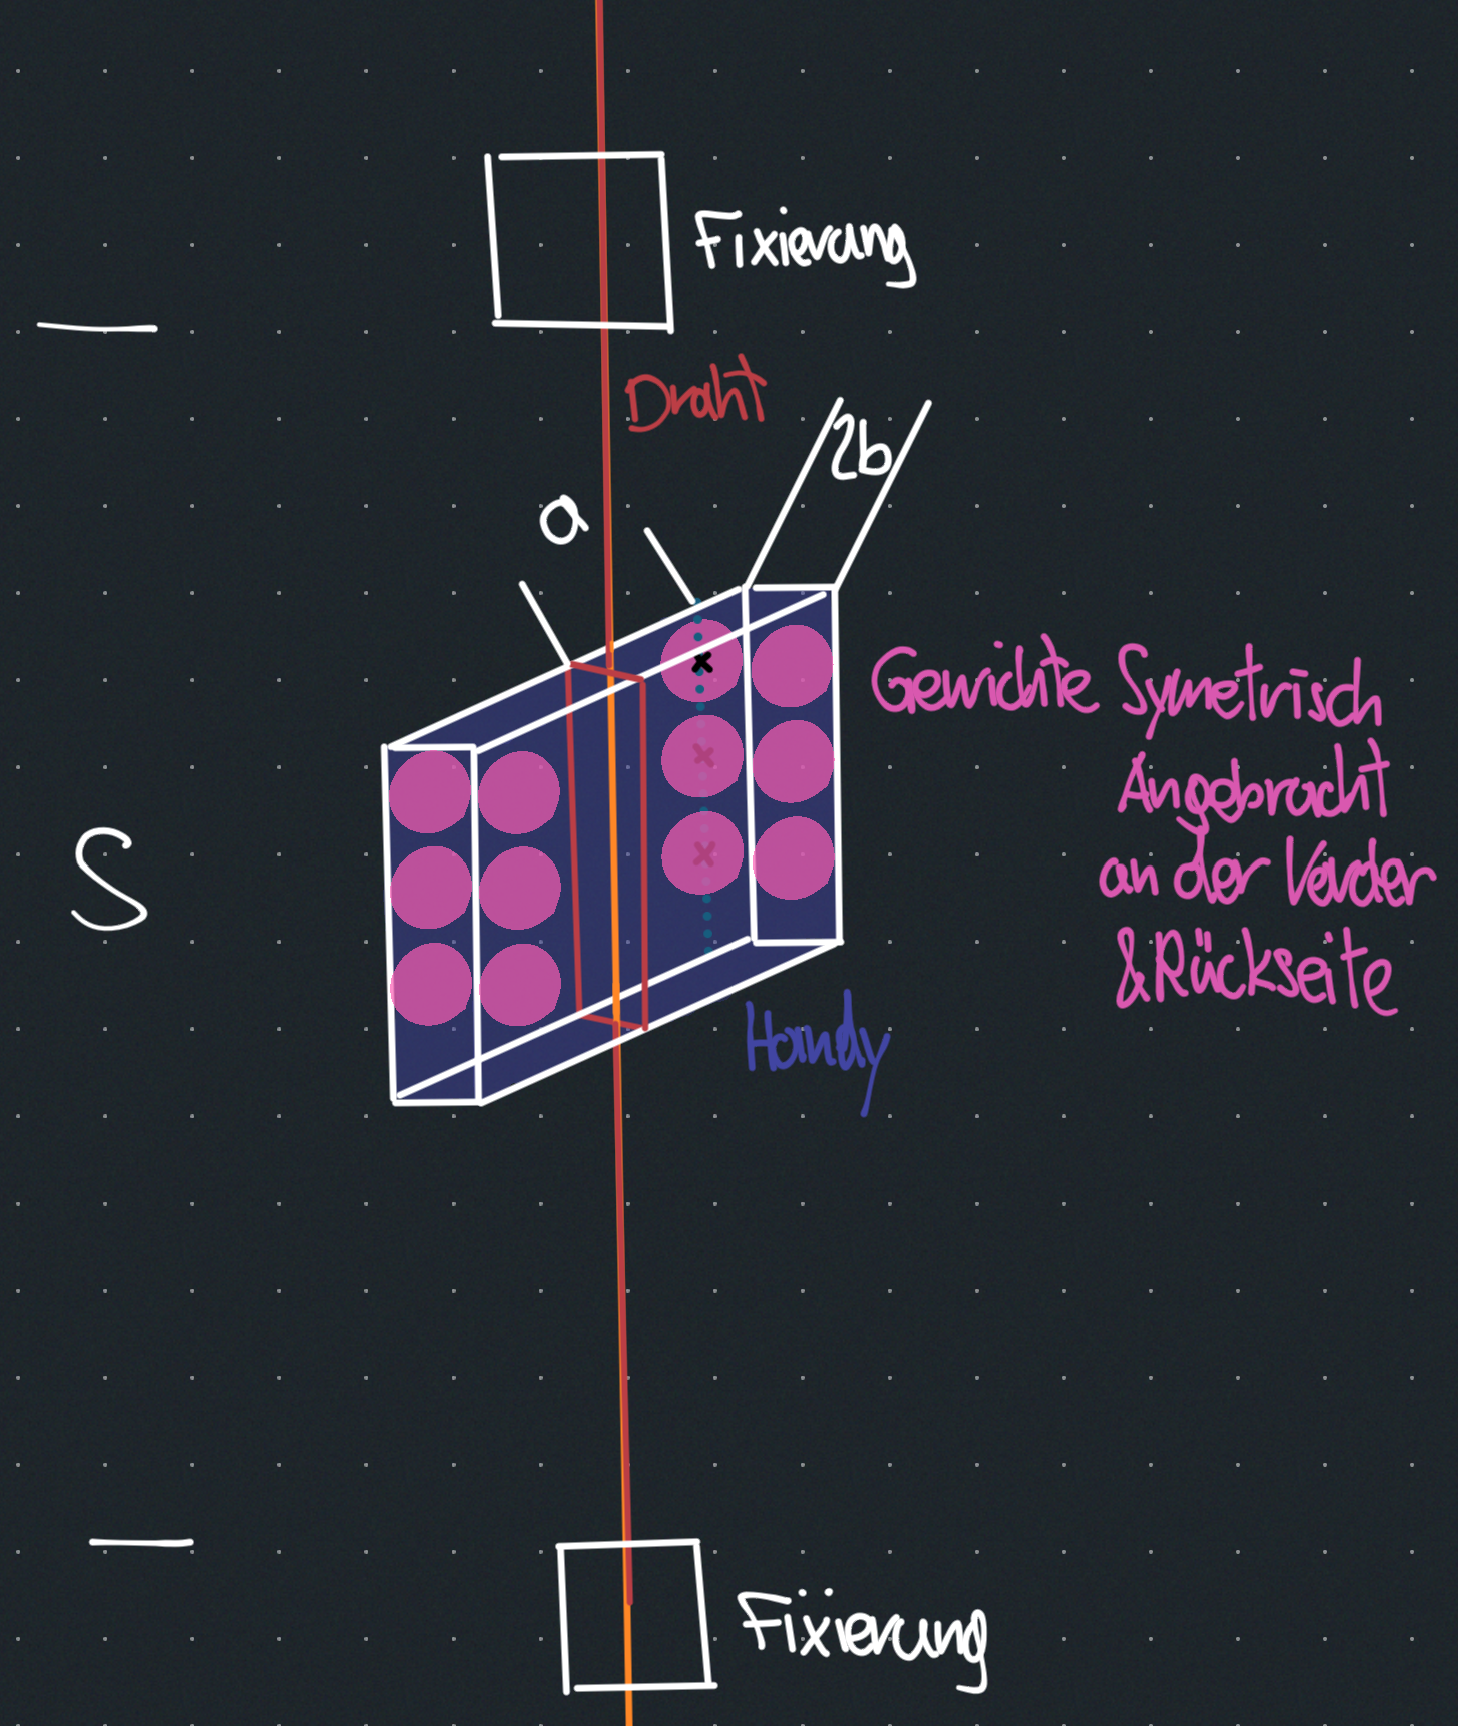
\includegraphics[width=0.8\linewidth]{pics/Skizze.png}
    \caption{Dies ist eine Skizze um die Verbindung zwischen 
    Theorie und Experiment zu visualisieren.}%
    \label{fig:Skizze}
\end{figure}

Unter Berücksichtigung einer Geschwindigkeitsabhängigen Reibung lautet die
Differentialgleichung der gedämpften Schwingung:

\begin{equation}
    \ddot \phi + 2\gamma \dot \phi + \omega_{0}^{2} \phi = 0
\end{equation}

wobei $\gamma$ die Dämpfungskonstante und $\omega_0 = \sqrt{\frac{D_r}{I}}$
die Kennfrequenz ist. Die Lösung der
gedämpften Schwingung lautet:

\begin{equation}
    \phi(t) = \phi_0 e^{-\gamma t} \cos{\omega_e t}
\end{equation}

Die Eigenfrequenz der Schwingung $\omega_e = \sqrt{\omega_{0}^{2} - \gamma^2}$
ist dabei durch die Dämpfung gegenüber der Kennfrequenz verringert worden. Im
Verlauf mehrerer Schwingungen verringert sich die Schwingungsamplitude nach
einer $e$-Potenz. Die Dämpfungskonstante $\gamma$ kann aus dem
Amplitudenverhältnis von aufeinanderfolgenden Schwingungen bestimmt werden zu:

\begin{equation}
    \frac{1}{t_P} \ln{(\frac{\phi(t)}{\phi(t+t_P)})} = \gamma \label{eq:gamma}
\end{equation}

Um zu sehen wie sich die Unsicherheit der Messungen bis in die Ergebnisse 
fortplanzt, ist \autoref{eq:Unsicherheitsfortpflanzung} verwendet worden.
Die Grundlagen dieser Gleichung sind von den Powerpointfolien von 
GUM entnommen worden.\cite{WolfgangKessel2004} Die Verallgemeinerung ist von Wikipedia entnommen
worden \cite{2020Fehler}.
Für die Auswertung ist die Progammiersprache Python im speziellen das 
Packet \verb#scipy#, zur Hilfe genommen worden.

\begin{equation}
    \label{eq:Unsicherheitsfortpflanzung}
    V_y = J(x) \cdot V_x \cdot J^{T}(x)
\end{equation}

Wobei $V_y$ und $V_x$ die Kovarianzmatrizen von den Vektoren $\bm{y}$ und $\bm{x}$.
$\bm{x}$ ist der Vektor der Eingangsvariablen und $\bm{y}$ ist der Vektor der Ausgangsvariabeln.
$J$ ist die Jakobimatrix der vektorwertigen Funktion $\bm{y} = \vec{F}(\bm{x})$ ist.
So lassen sich die Komponent der Matrix relativ einfach anschreiben $J_{ij}(x) = \frac{\partial{y_i}}{\partial{x_j}}(x)$.
Damit man die Unsicherheit der einzelnen Variabeln $y_i$ bekommt muss nur die Quadratwurzel des i-ten Diagonalelementes der 
$\bm{y}$-Kovarianzmatrix genommen werden $u_i= \sqrt{\mathrm{diag}(V_y)_i}$.
Da in diesem Experiment meistens nur skalare Funktionen untersucht werden vereinfacht
sich die \autoref{eq:Unsicherheitsfortpflanzung} dramatisch und die Unsicherheit
der Variabel $y$ lässt sich einfach so berechnen:

\begin{equation}
    \label{eq:graduncentainty}
    u_y = \sqrt{\mathrm{grad} y^T \cdot V_x \cdot \mathrm{grad} y}
\end{equation}

\section{Versuchsanordnung}
\label{sec:versuchsanordnung}

Das Handy wird in einem Stahldraht eingewickelt und zwischen zwei Beinen eines
Sessels eingespannt. Ein Schraubenzieher wird verwendet um den Draht zu
spannen.  Dieser wurde so eingesetzt, dass das Gewicht des Sessel auf den
Schraubenzieher lastet und damit immer stärker den Draht spannt. Für den ersten
Teilversuch wird nur das Handy selbst ausgelenkt, für die folgenden Versuche
werden erst ohne dann insgesamt 4, dann insgesamt 8 und dann insgesamt 12
50-Cent Münzen am Handy fixiert. Dabei wird vom unteren Rand des Handys
angefangen und es werden jeweils immer auf der linke und rechten äußeren Seite
die Münzen mit Klebeband symetrisch fixiert, damit sich der Schwerpunkt nicht
verschiebt, siehe \autoref{fig:Aufbau}.

\begin{figure}[H]
    \centering
    \begin{minipage}[htbp]{\linewidth}
        \begin{minipage}[htbp]{.32\linewidth} % [b] => Ausrichtung an \caption
            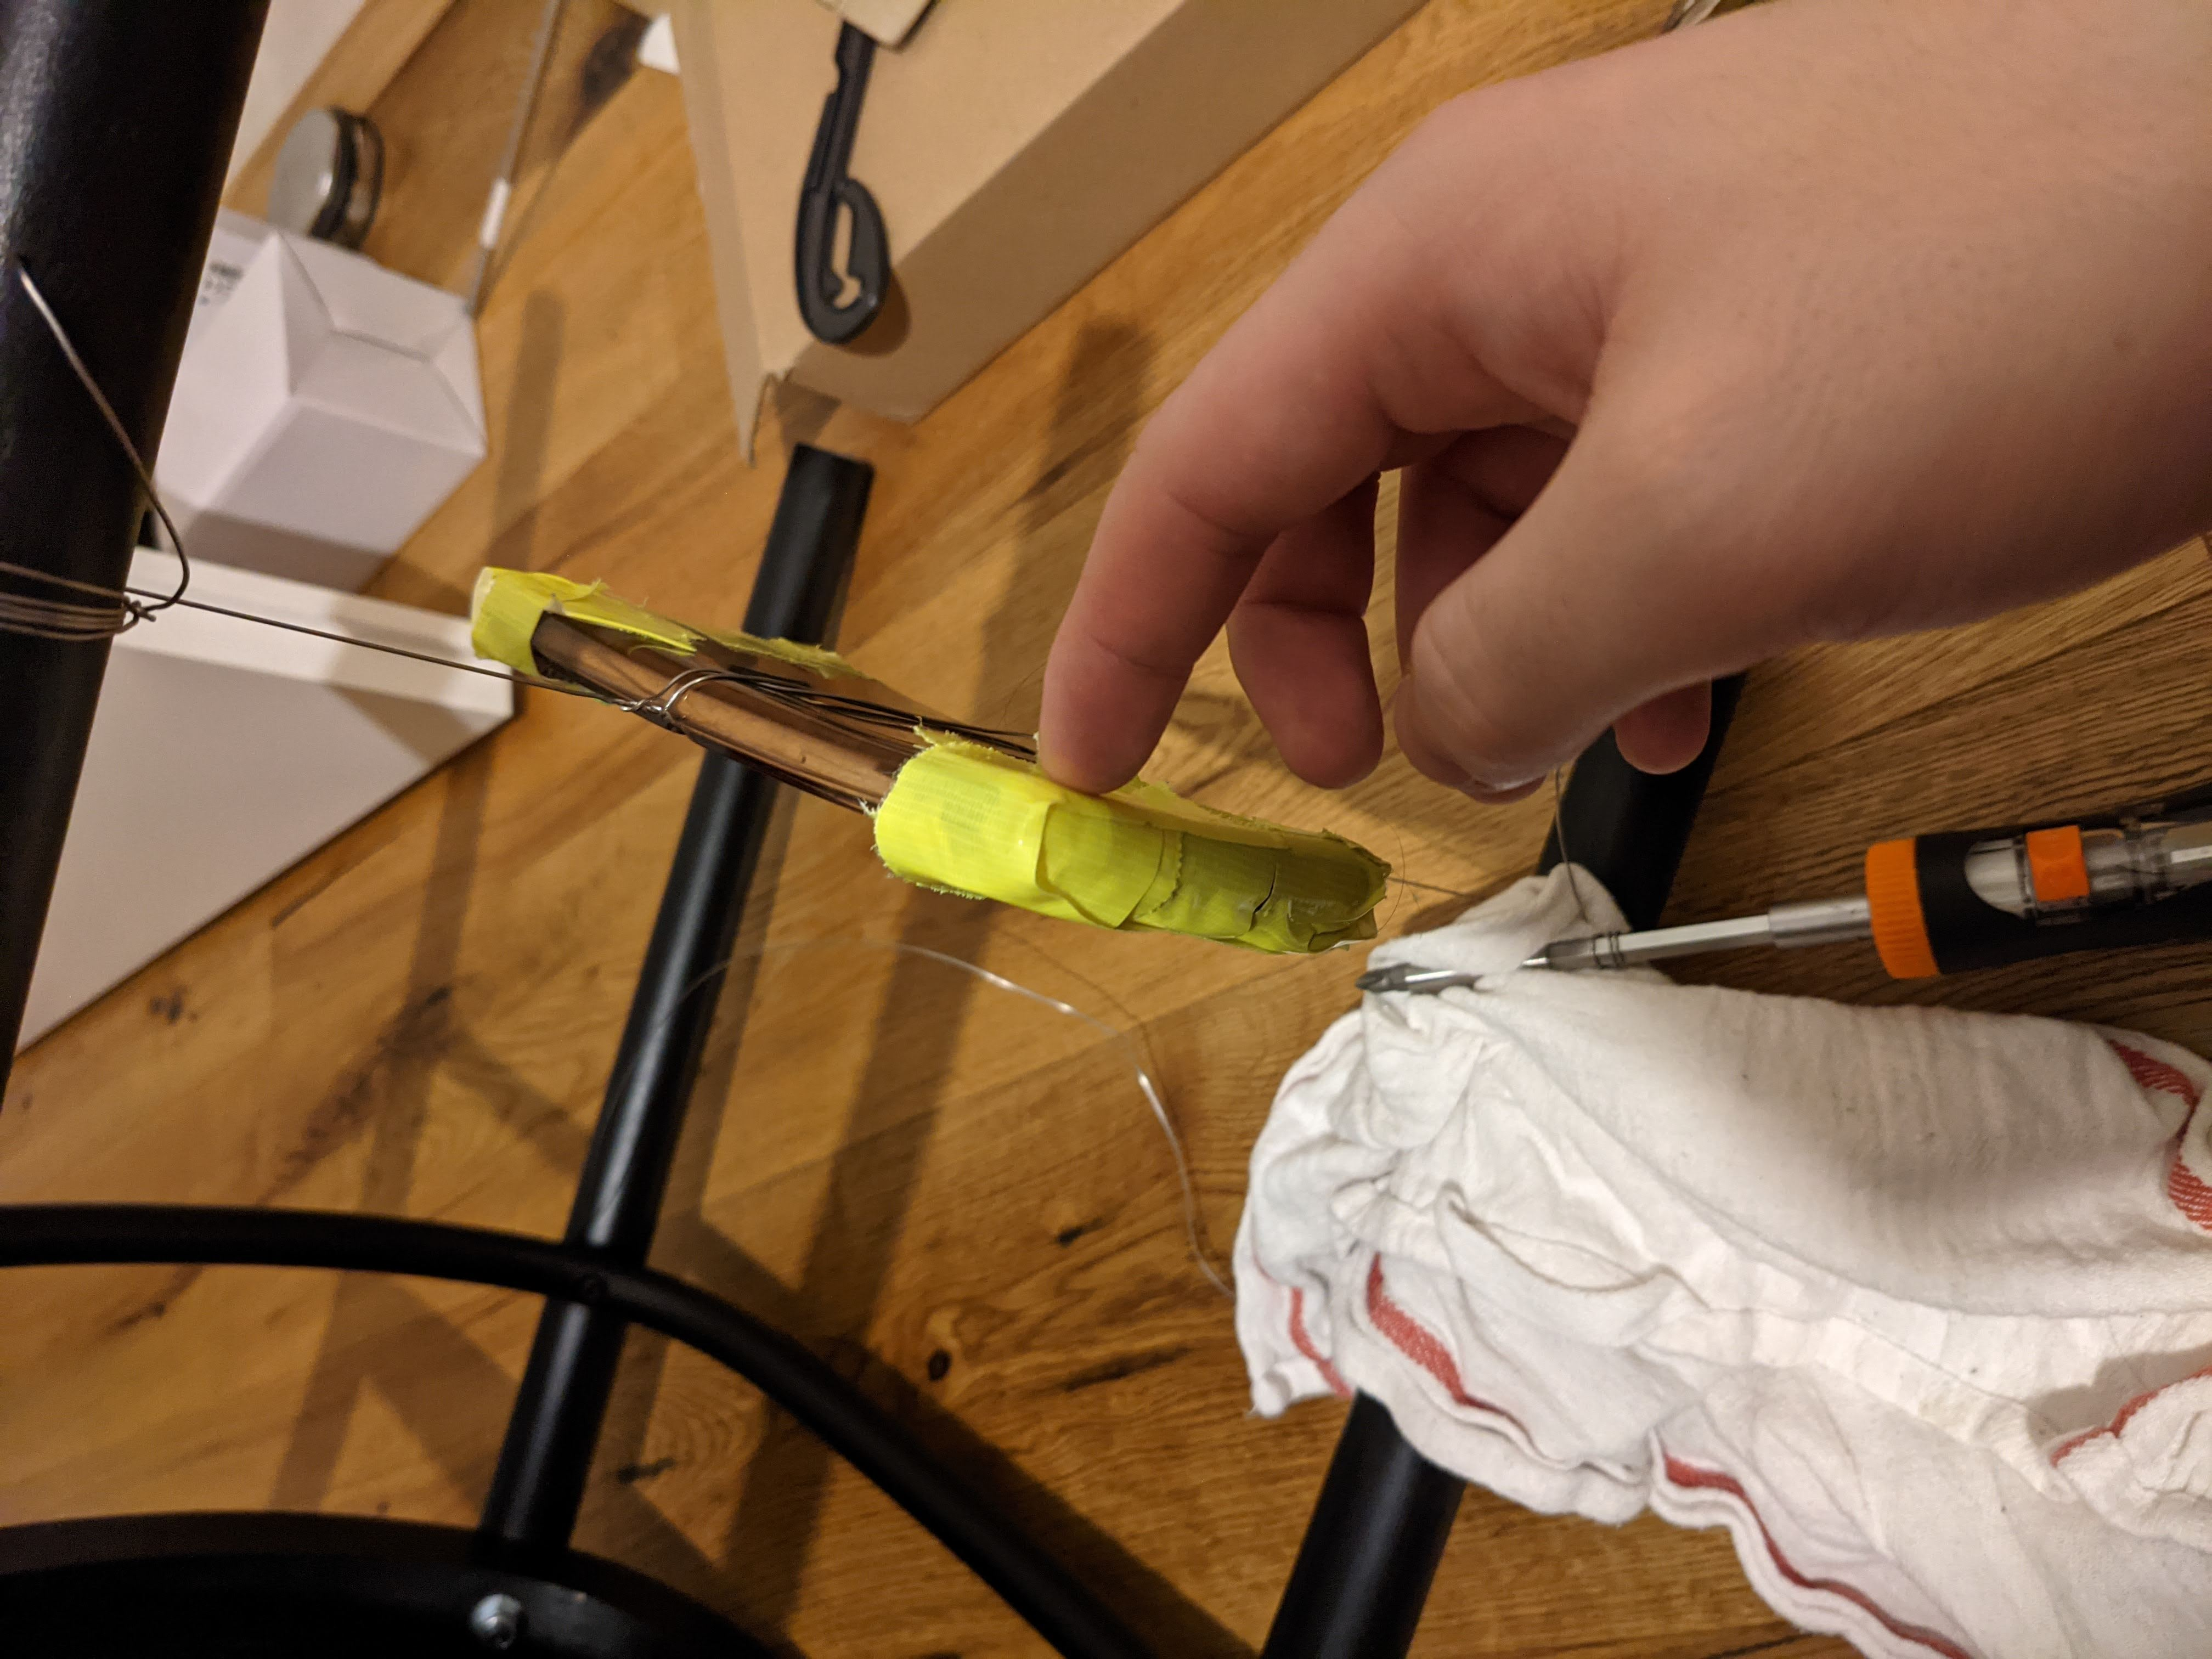
\includegraphics[angle=-90,origin=c,width=\linewidth]{pics/Aufbau (1).jpg}
        \end{minipage}
        \begin{minipage}[htbp]{.32\linewidth} % [b] => Ausrichtung an \caption
            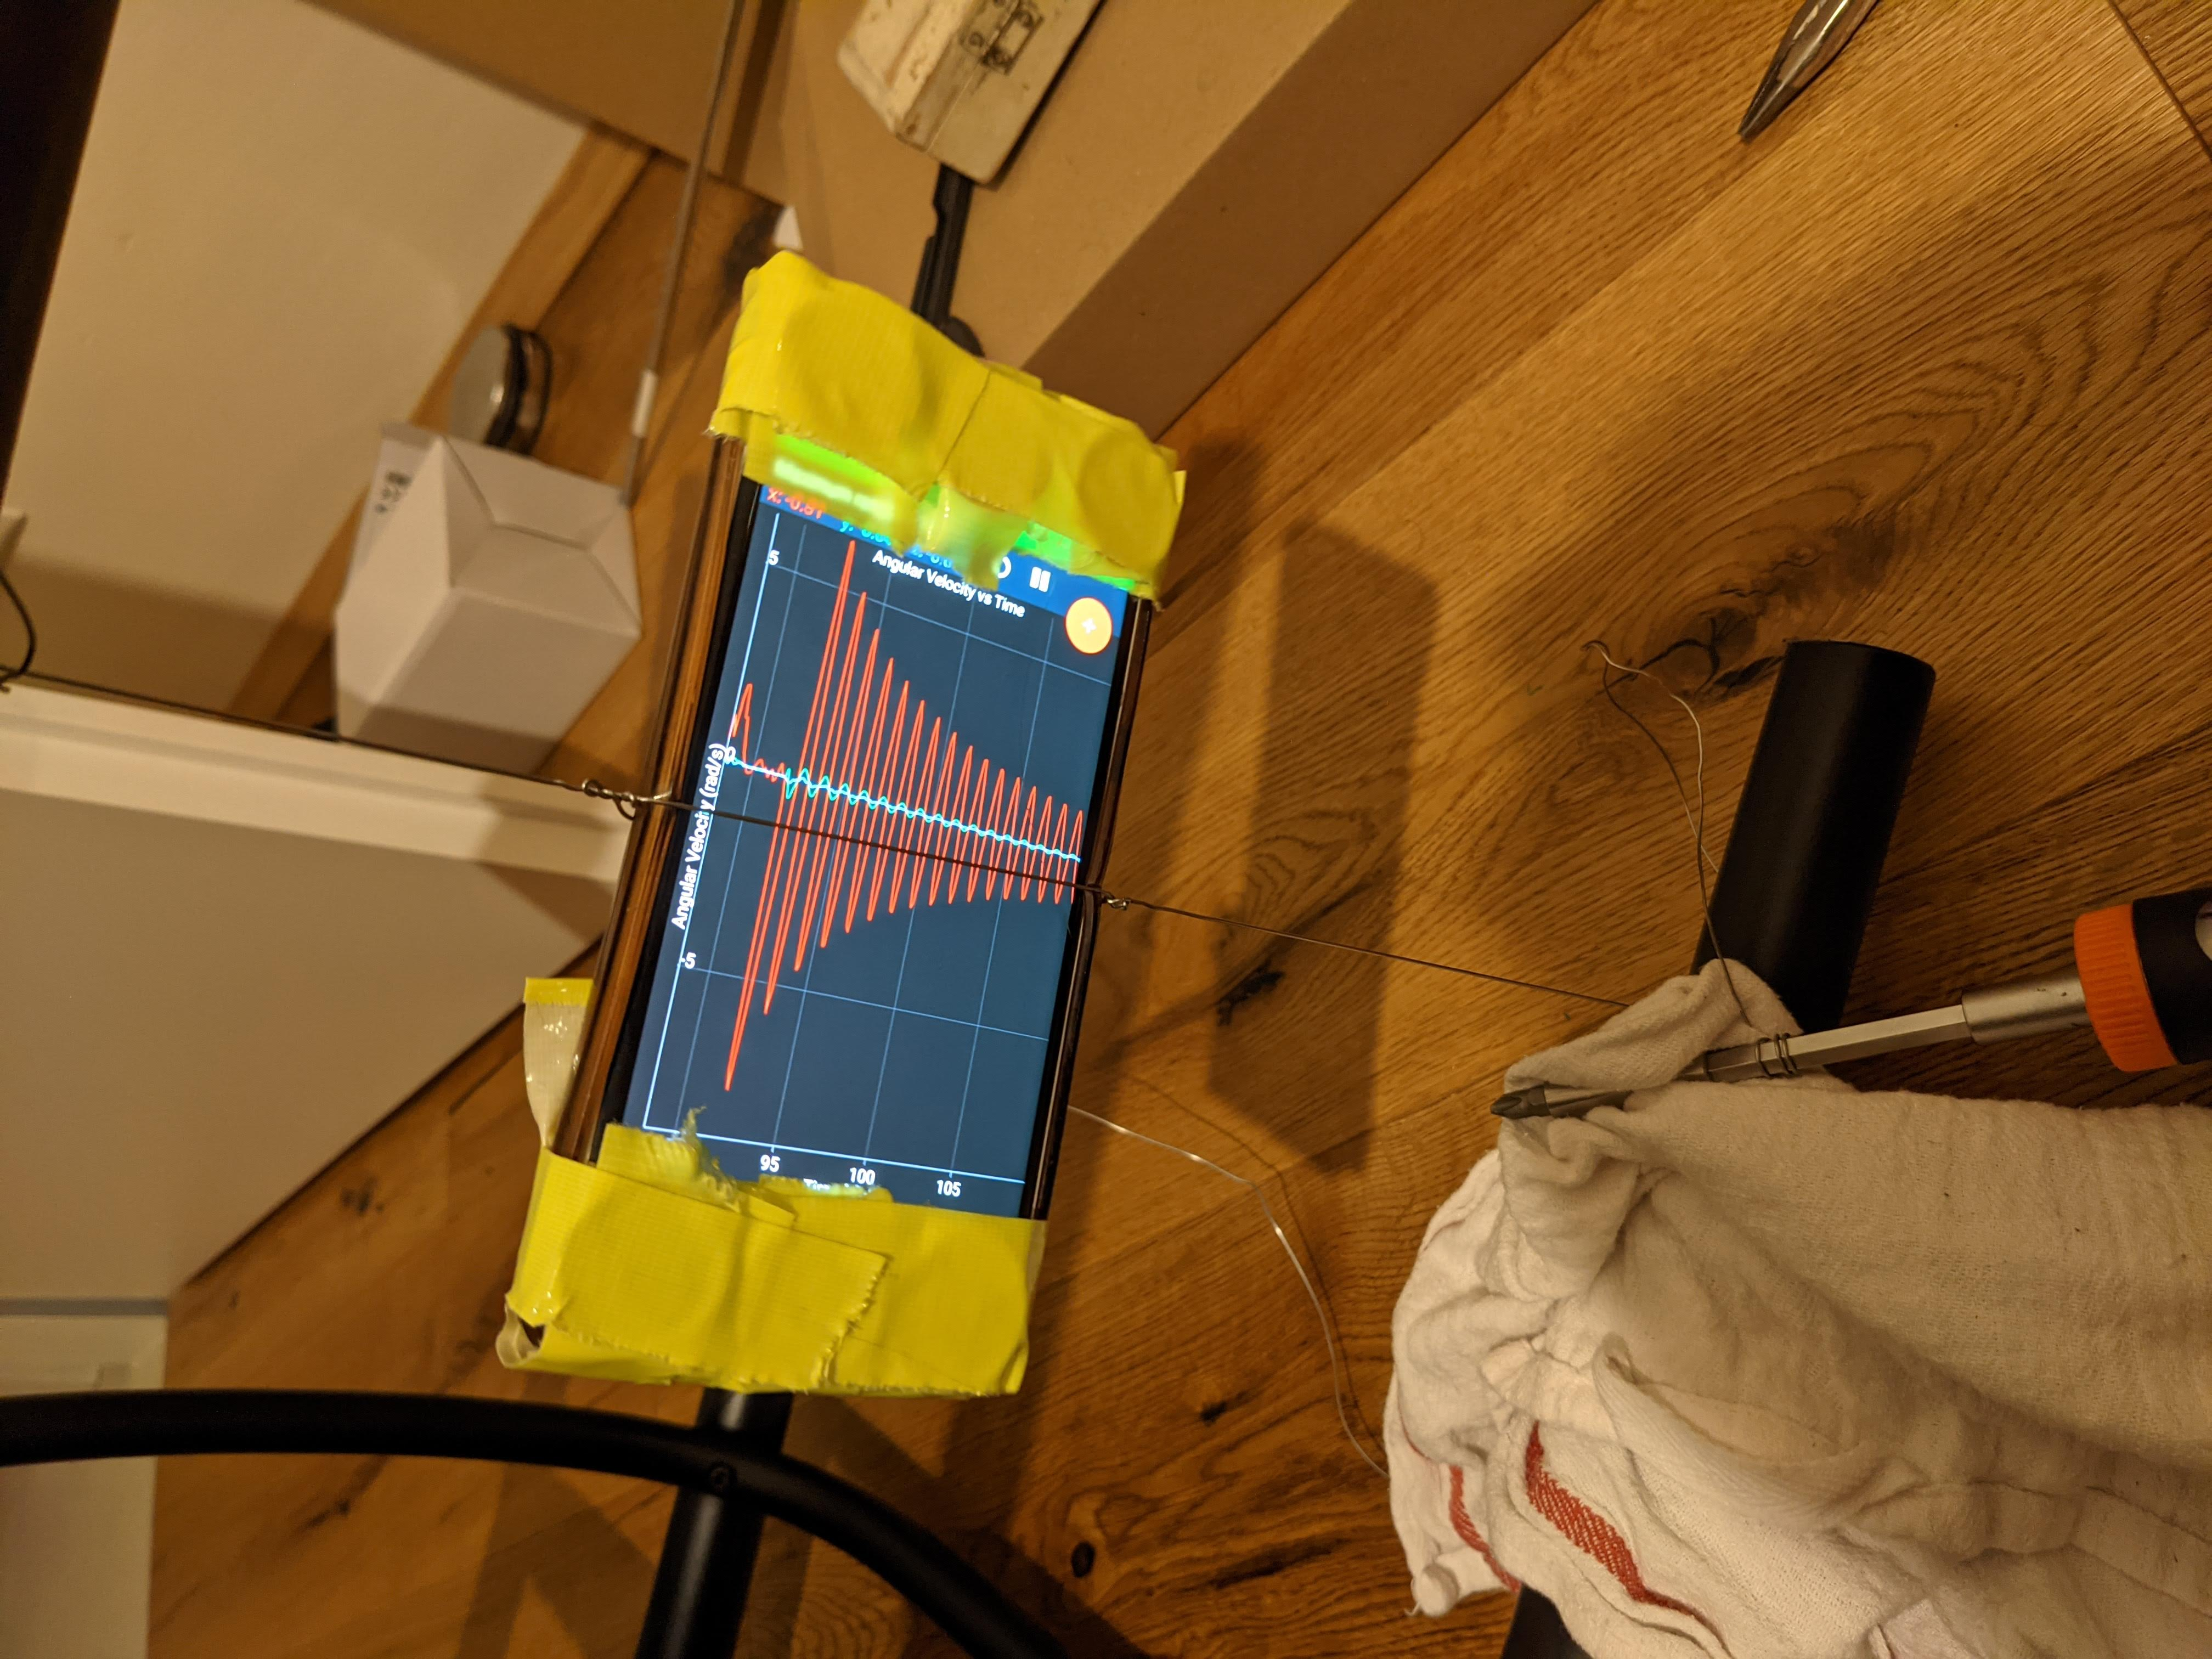
\includegraphics[angle=-90,origin=c,width=\linewidth]{pics/Aufbau (2).jpg}
        \end{minipage}
        \begin{minipage}[htbp]{.32\linewidth} % [b] => Ausrichtung an \caption
            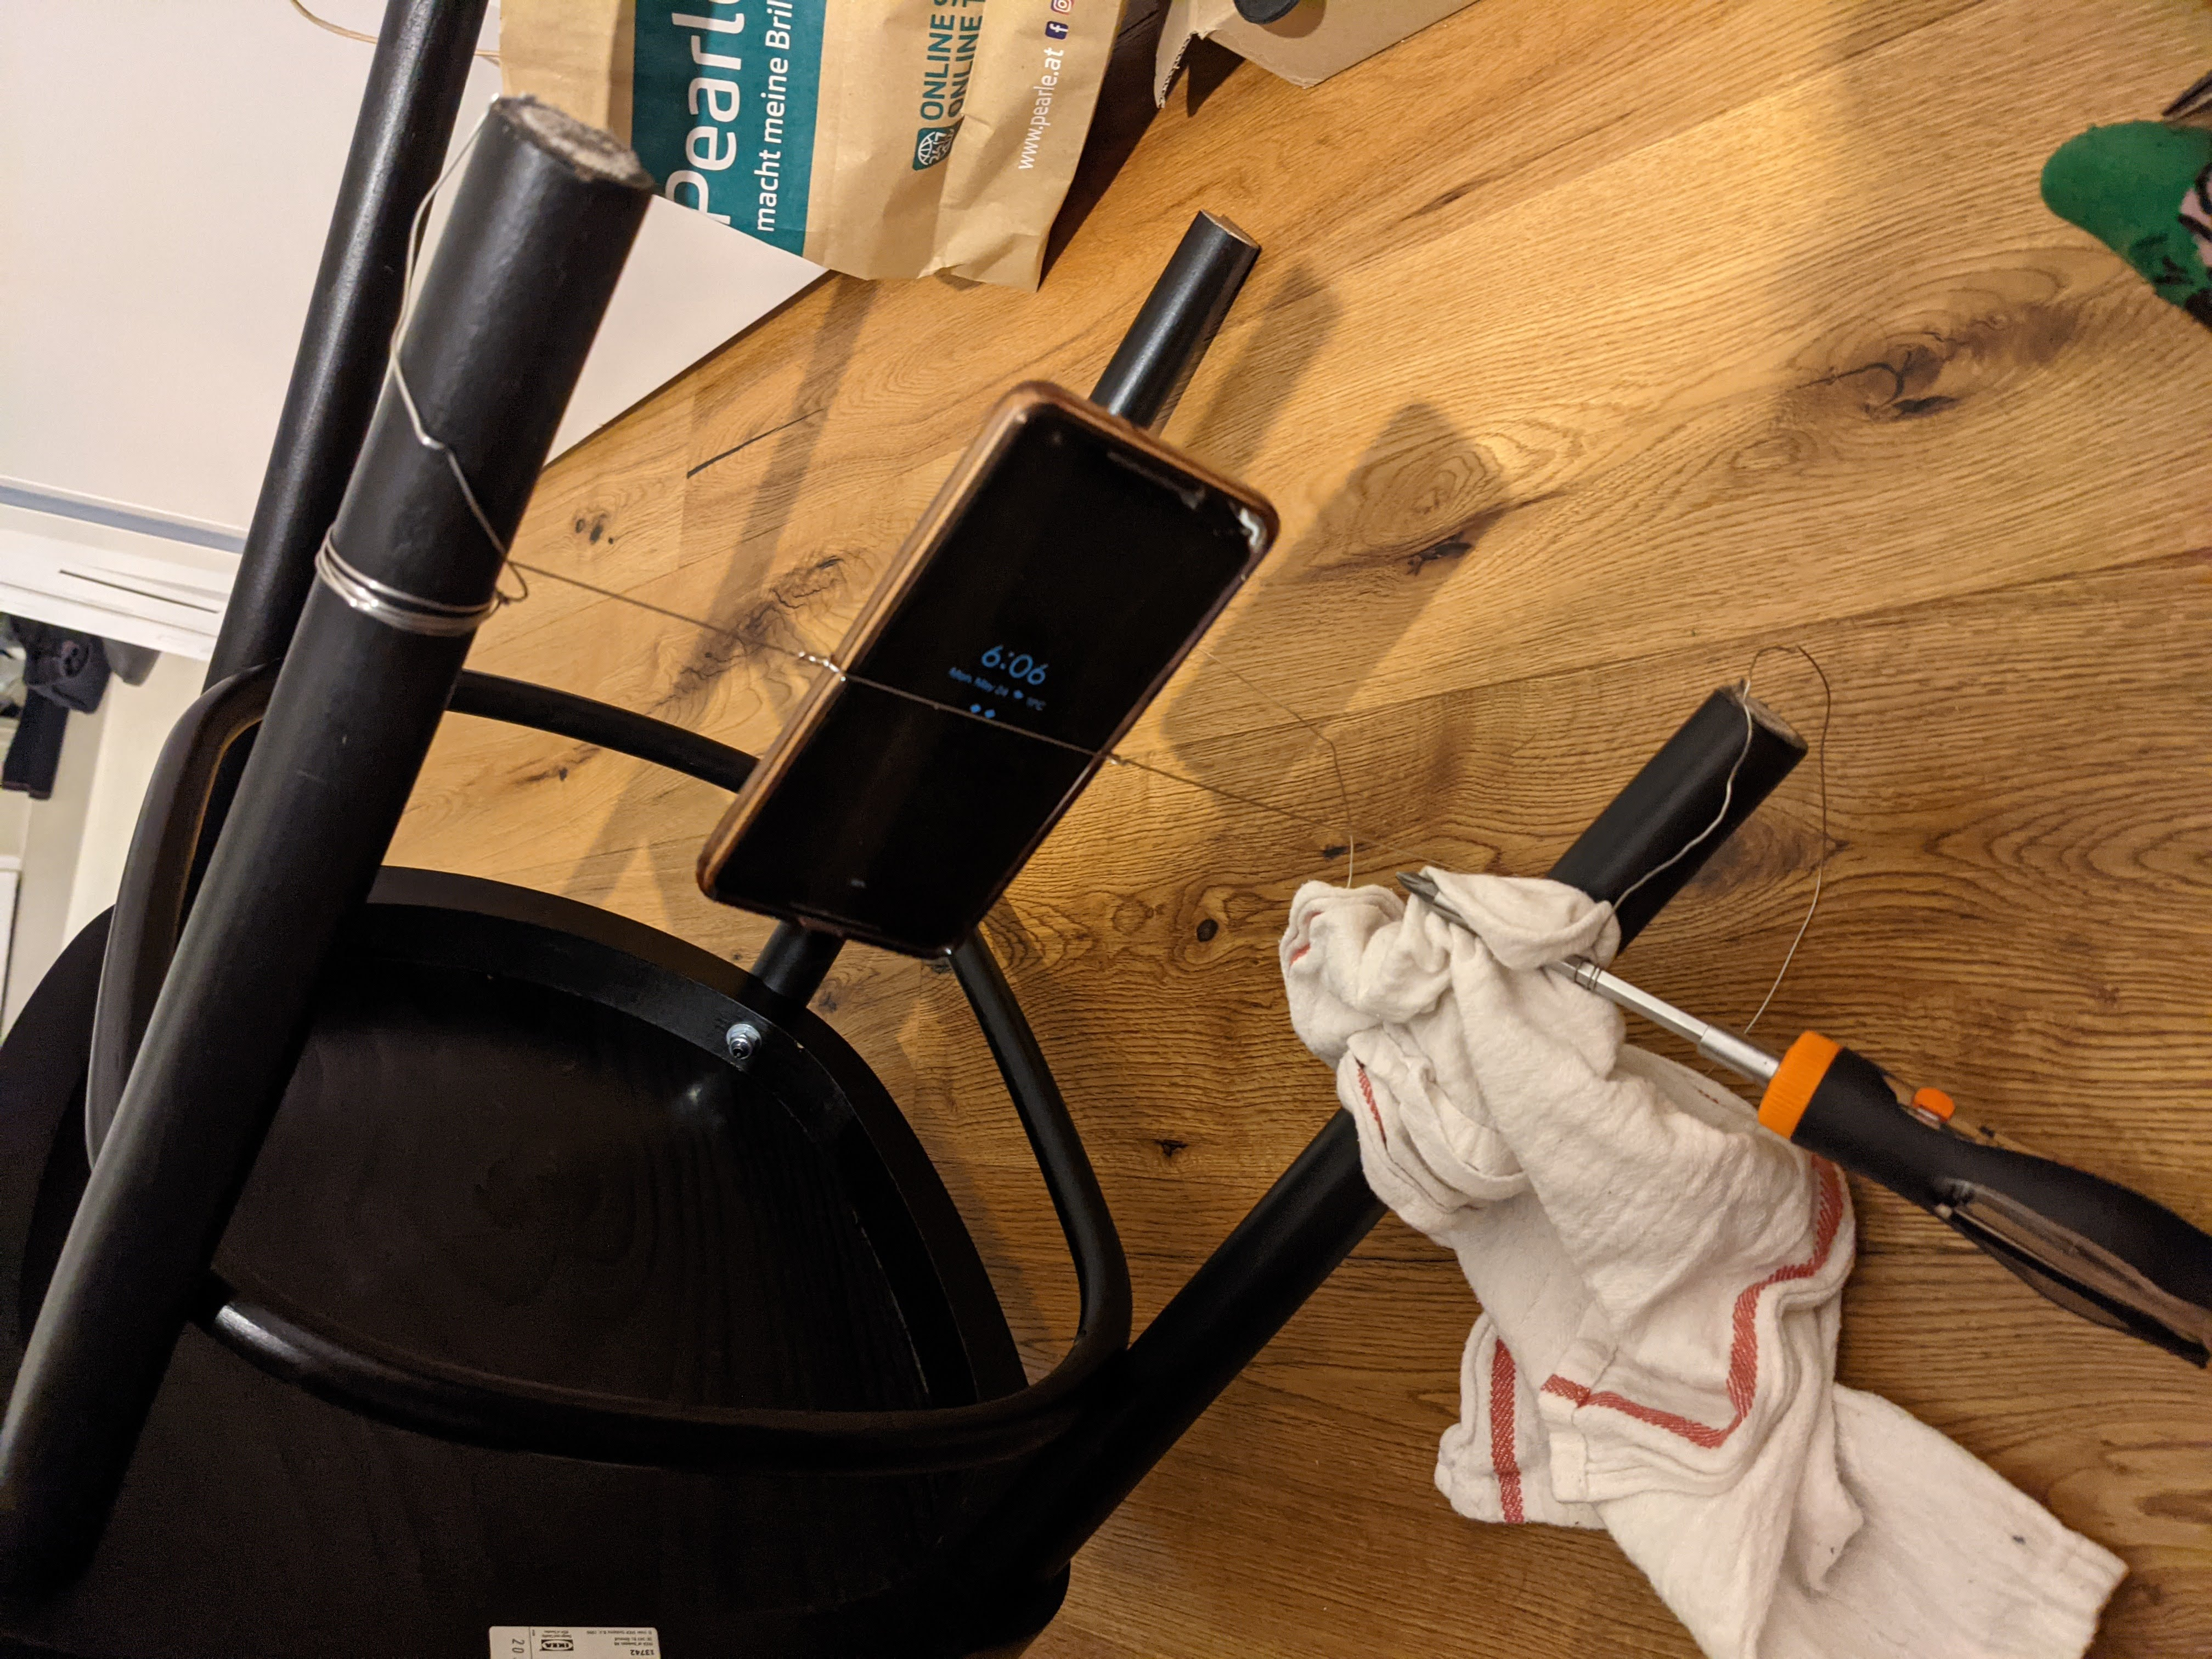
\includegraphics[angle=-90,origin=c,width=\linewidth]{pics/Aufbau (3).jpg}
        \end{minipage}
        \caption[Aufbau des Experiments]{3 Messungen der Winkelgeschwindigkeit $\omega_{x}$ in der x-Achse des Smartphones ohne Zusatzgewichte}
        \label{fig:Aufbau}
    \end{minipage}
 \end{figure}


\section{Geräteliste}
\label{sec:geraeteliste}
%\setlength\LTleft{-6.5em}
\begin{longtable}{c|c|S|p{15em}}
\caption[Geräteliste]{Verwendete Geräte \label{tab:geraeteliste}} \\  % optionales Argument wird in Verzeichnissen verwendet, essentielles Argument direkt im Text
\toprule
Gerät                              & Gerät-Nr. & { Unsicherheit }  & Bemerkungen \\  
\midrule
\endfirsthead
\caption[]{(Fortsetzung)}\\
\toprule
Gerät                              & Gerät-Nr. & { Unsicherheit }  & Bemerkungen \\                                                                        
\midrule
\endhead
\endfoot
\endlastfoot
        Handy              & axx & \SI{3}{\ms}             & Wird verwendet um Winkelgeschwindigkeit aufzuzeichnen und es ist das Objekt von dem, das Trägheitsmoment bestimmt wird.                               \\ \hline
        Maßband            & bxx & \SI{1}{\mm}       & - \\ \hline
        Schublehre         & cxx & \SI{0.02}{\mm}       & Um die Dicke bzw. Länge des Smartphones zu messen \\ \hline
        50-Cent-Münzen 12x & dxx & { - }     & Die Zusatzgewichte von denen man das Trägheitsmoment leicht berechnen kann.\\ \hline
        Stuhl              & gxx & { - }             & Zum Befüllen des Quincke-Rohres                                                       \\ \hline
        Stahldraht         & hxx & { - } & Sendet einen \SI{1600.00}{\hertz} Sinussignal an den Lautsprecher                     \\ \hline
        Schraubenzieher    & ixx & { - }             & Zum Anregen von stehenden Wellen im Quincke-Rohr mit der Frequenz vom Signalgenerator \\ \hline
        Thermometer        & jxx & \SI{0.6}{\kelvin} & Modell: GTH 1170 (Greisinger GmbH.) Um die Umgebungstemperatur zu bestimmen           \\ \hline

        \hline
\end{longtable}

\section{Versuchsdurchführung und Messergebnisse}
\label{sec:versuchsdurchfuehrung_messergebnisse}
Die 50 Cent-Münzen haben ein Gewicht \SI{7.80}{\g}, einen Durchmesser von
\SI{24.25}{\mm} und eine Dicke von \SI{2.38}{\mm}, siehe \cite{50cent}.
Der Fehler wurde als implizit angegeben Angenommen.

Weiters sind die Länge $a$ und $b$, aus der Skizze \ref{fig:Skizze} mit der
Schublehre bestimmt worden.  $a$ ist \SI{67(2)}{\mm} und $b$ ist
\SI{8.35(4)}{\mm}. Da die Befestigung nicht so exakt war kann $a$ nicht so
genau bestimmt werden. 

Das eingespannte Handy wird per Hand um \num{90(2)} Grad ausgelenkt und
losgelassen und das Handy zeichnet de Winkelgeschwindigkeit auf. Nach \num{10}
Schwingungen (bei der Unbelasteten) war die Amplitude der Winkelschwingung nur
mehr \SI{27(1)}{\percent} von der Initialen. 

Im nächsten Schritt werden am
unteren Rand des Handys auf beiden Seiten je zwei 50-Cent Münzen mit Klebeband
fixiert, siehe \autoref{fig:Skizze}. Nun wird das Handy mit den Münzen
ausgelenkt und das Hany zeichnet wieder die Winkelgeschwindigkeit auf.  Dies
wird nun weitere zweimal wiederholt, wobei beim zweiten Mal die Münzen rechts
und links am mittleren Rand fixiert werden und beim dritten Mal am oberen Rand.
Somit erhält man folgende Daten.


\begin{figure}[H]
    \centering
    \begin{minipage}[htbp]{\linewidth}
        \begin{minipage}[htbp]{.32\linewidth} % [b] => Ausrichtung an \caption
            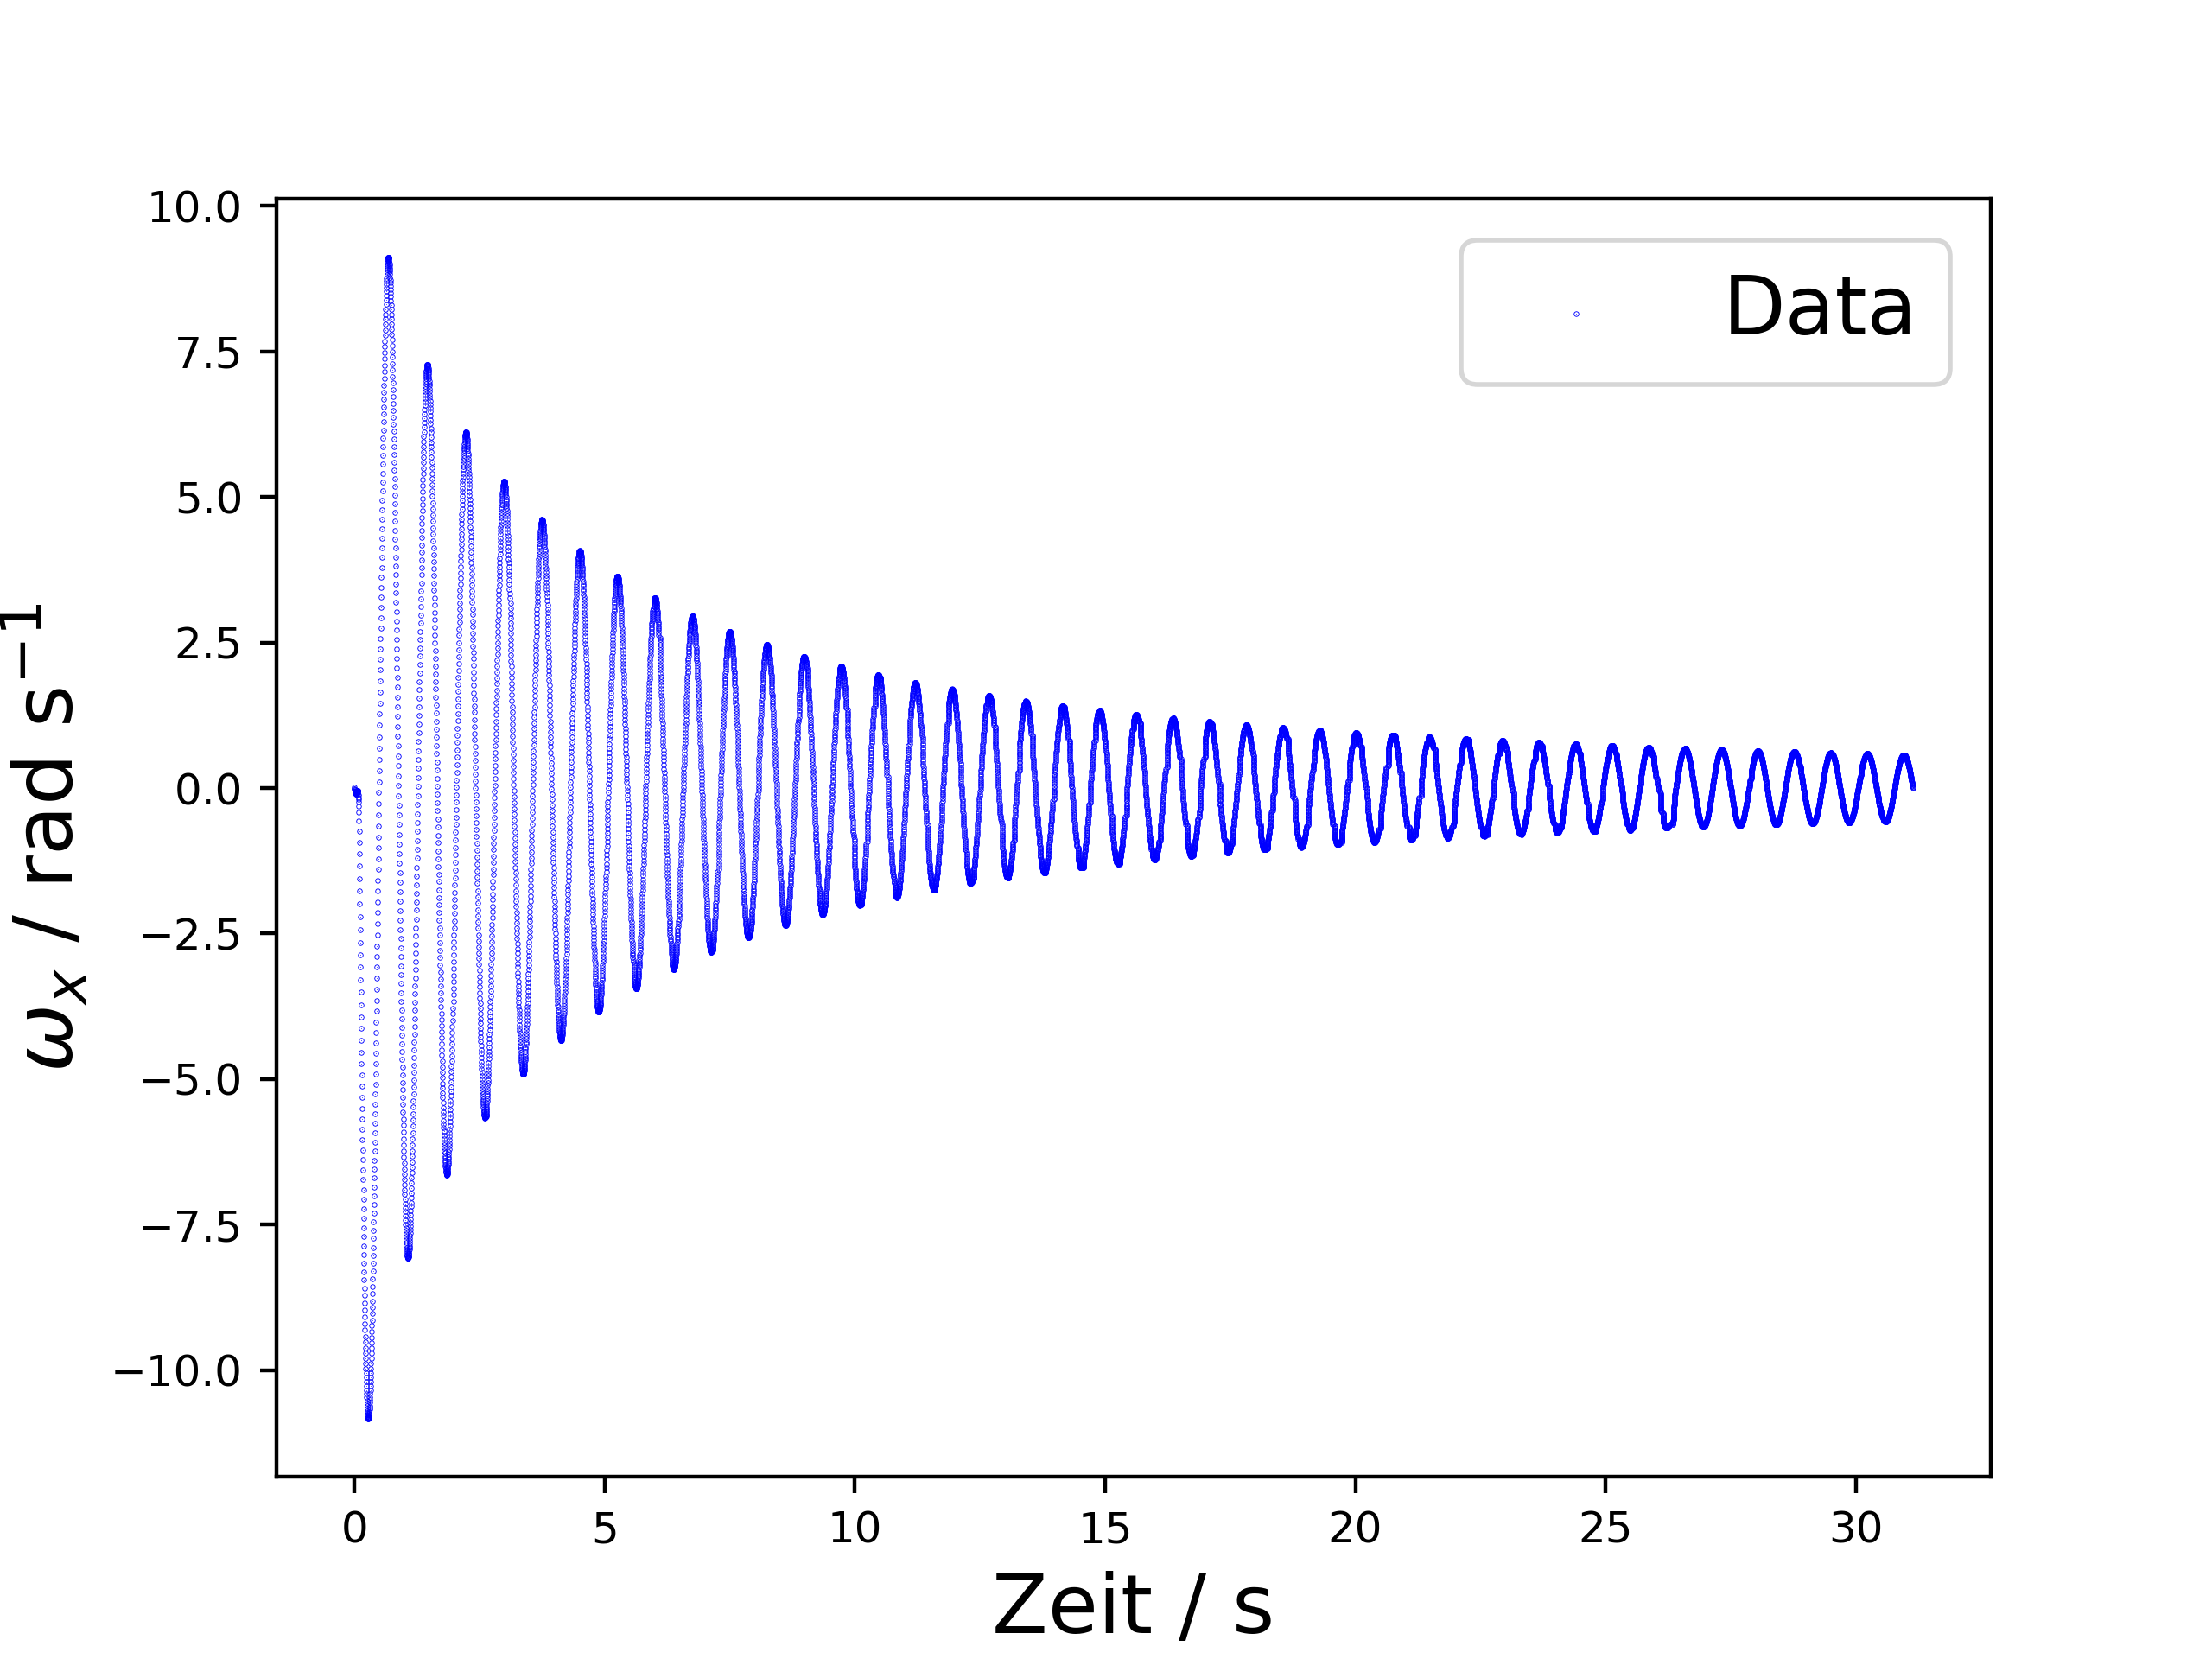
\includegraphics[width=\linewidth]{pics/omega/fit_of_t_wx_mess_nr_1.png}
        \end{minipage}
        \begin{minipage}[htbp]{.32\linewidth} % [b] => Ausrichtung an \caption
            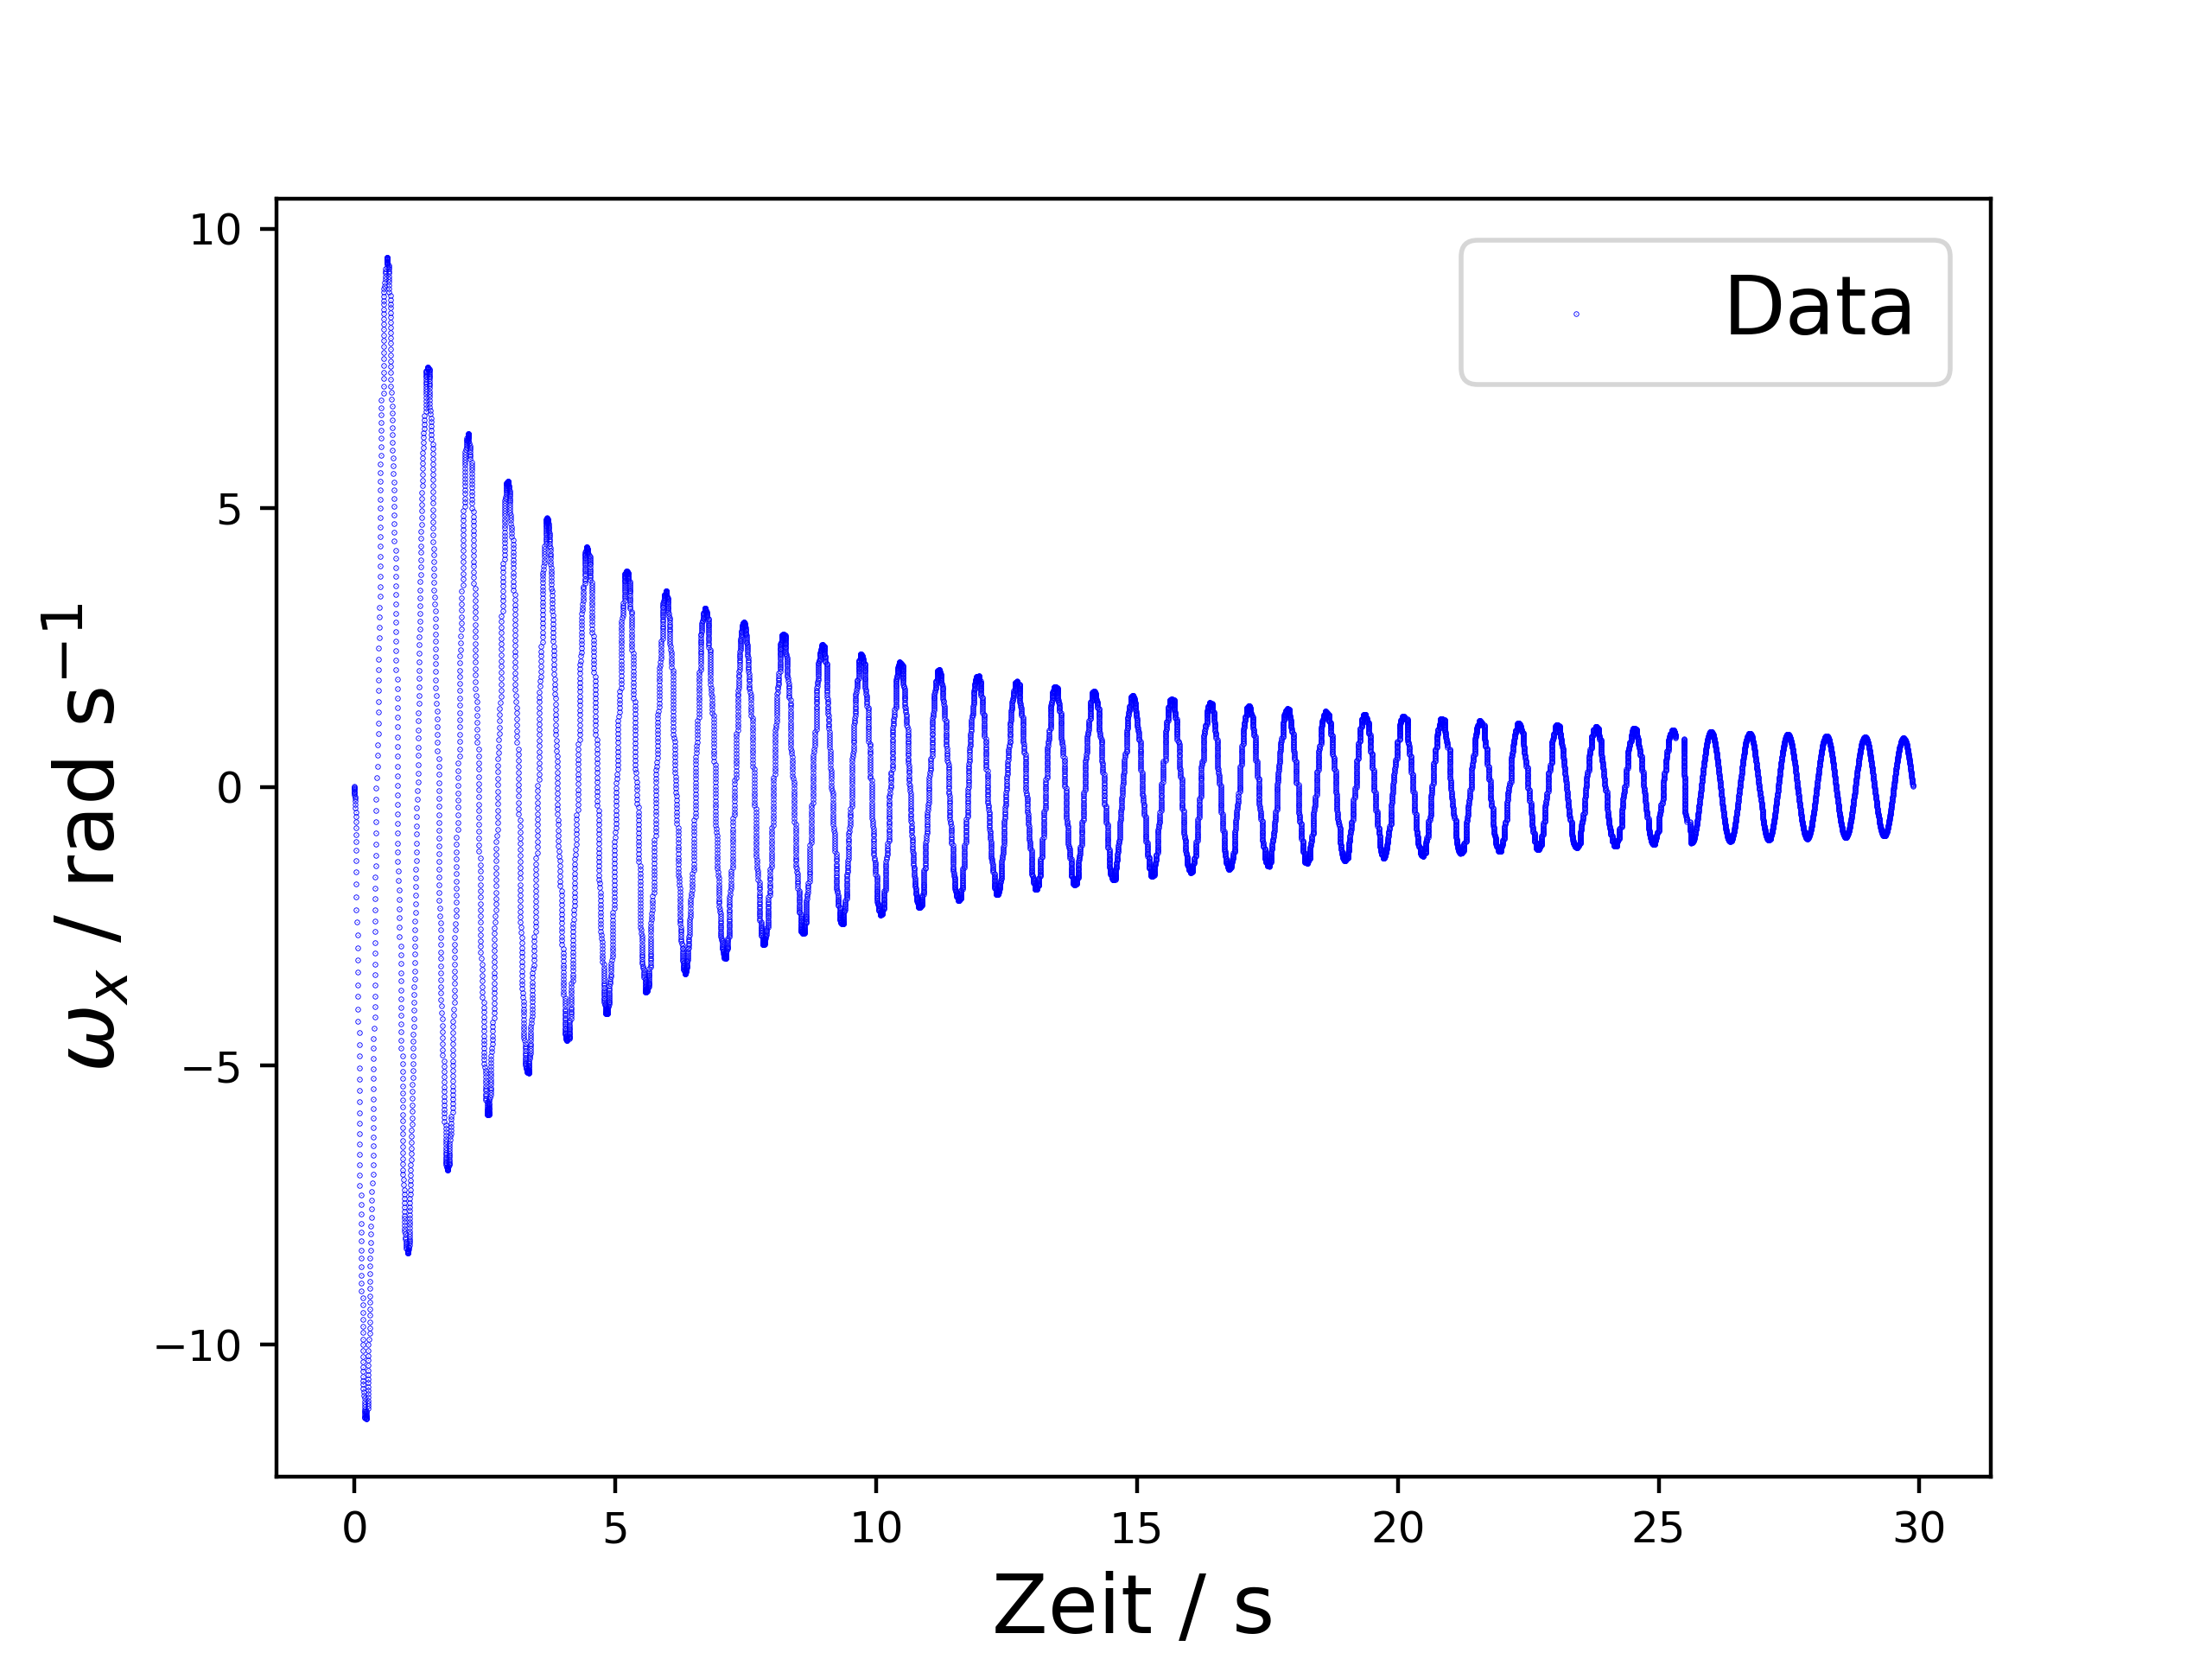
\includegraphics[width=\linewidth]{pics/omega/fit_of_t_wx_mess_nr_2.png}
        \end{minipage}
        \begin{minipage}[htbp]{.32\linewidth} % [b] => Ausrichtung an \caption
            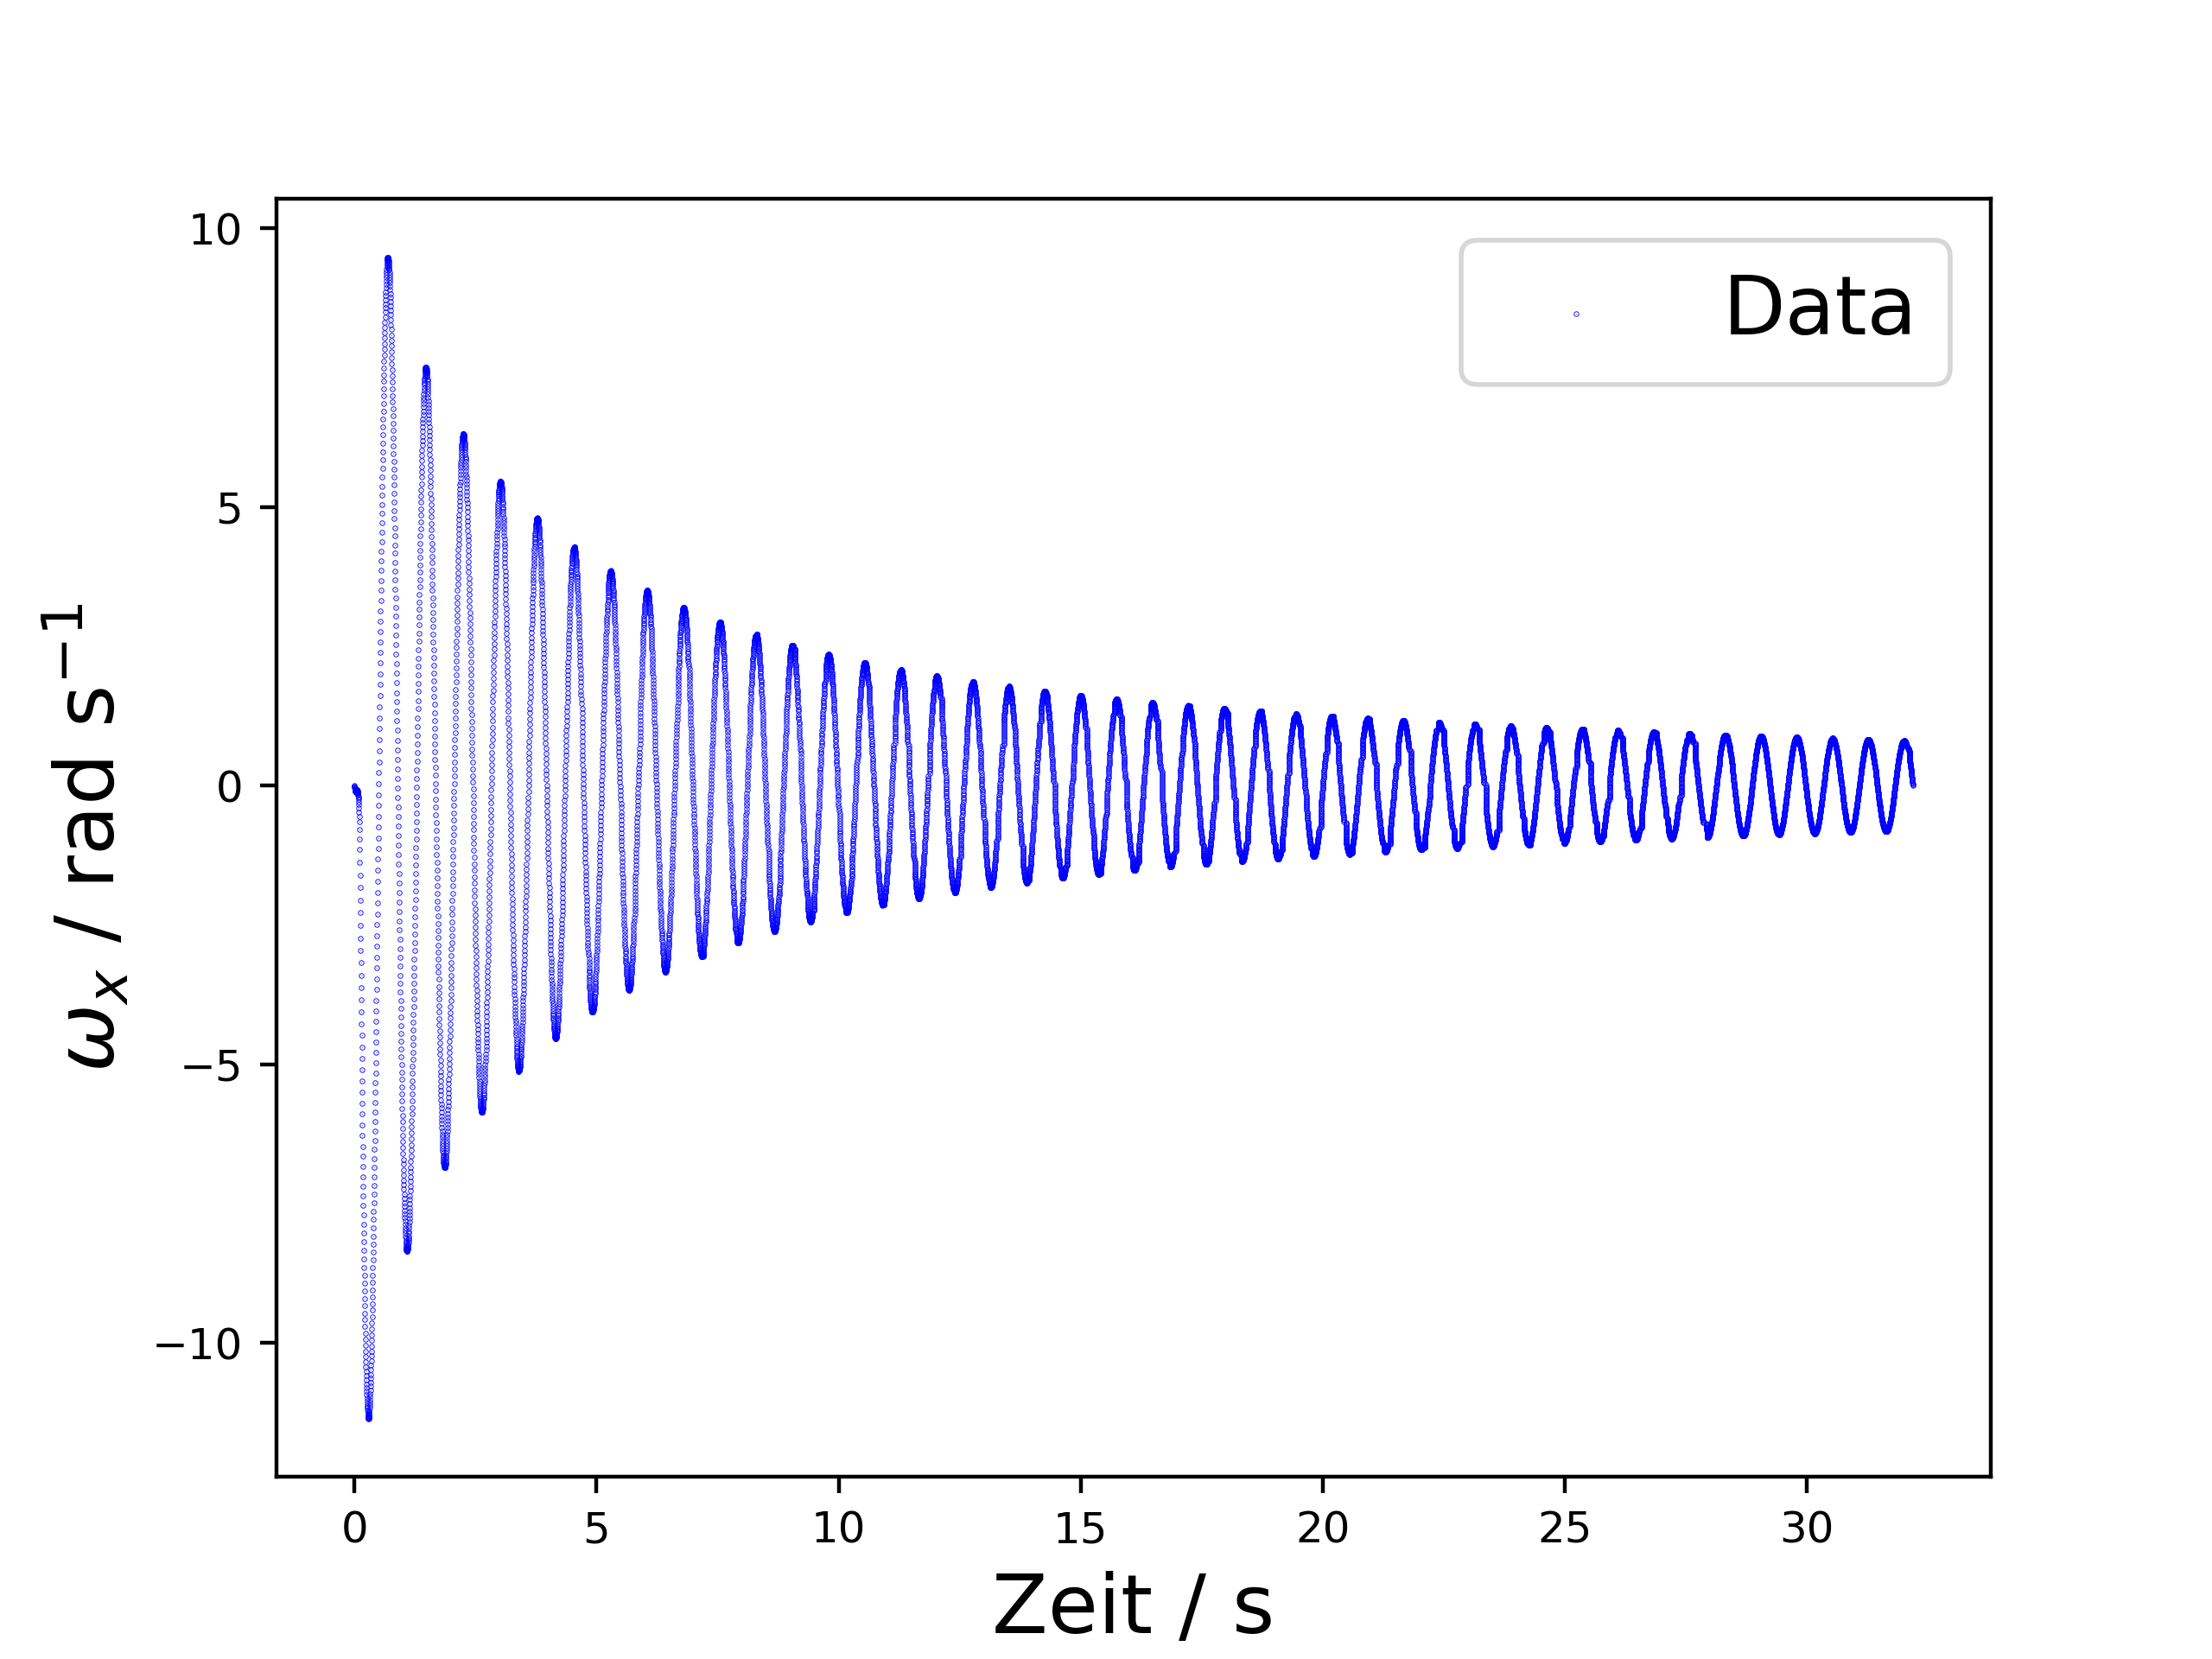
\includegraphics[width=\linewidth]{pics/omega/fit_of_t_wx_mess_nr_3.png}
        \end{minipage}
        \caption[Schwingungsmessungen ohne Zusatzgewichte]{3 Messungen der Winkelgeschwindigkeit $\omega_{x}$ in der x-Achse des Smartphones ohne Zusatzgewichte.
        Wobei auf der x-Achse die Zeit $t$ / \si{\second} aufgetragen wurde und auf der y-Achse die Winkelgeschwindigkeit $\omega_x$ / \si{\radian\per\second} }
        \label{fig:ohne}
    \end{minipage}
 \end{figure}

\newpage

\begin{figure}[H]
    \centering
    \begin{minipage}[htbp]{\linewidth}
        \begin{minipage}[htbp]{.32\linewidth} % [b] => Ausrichtung an \caption
            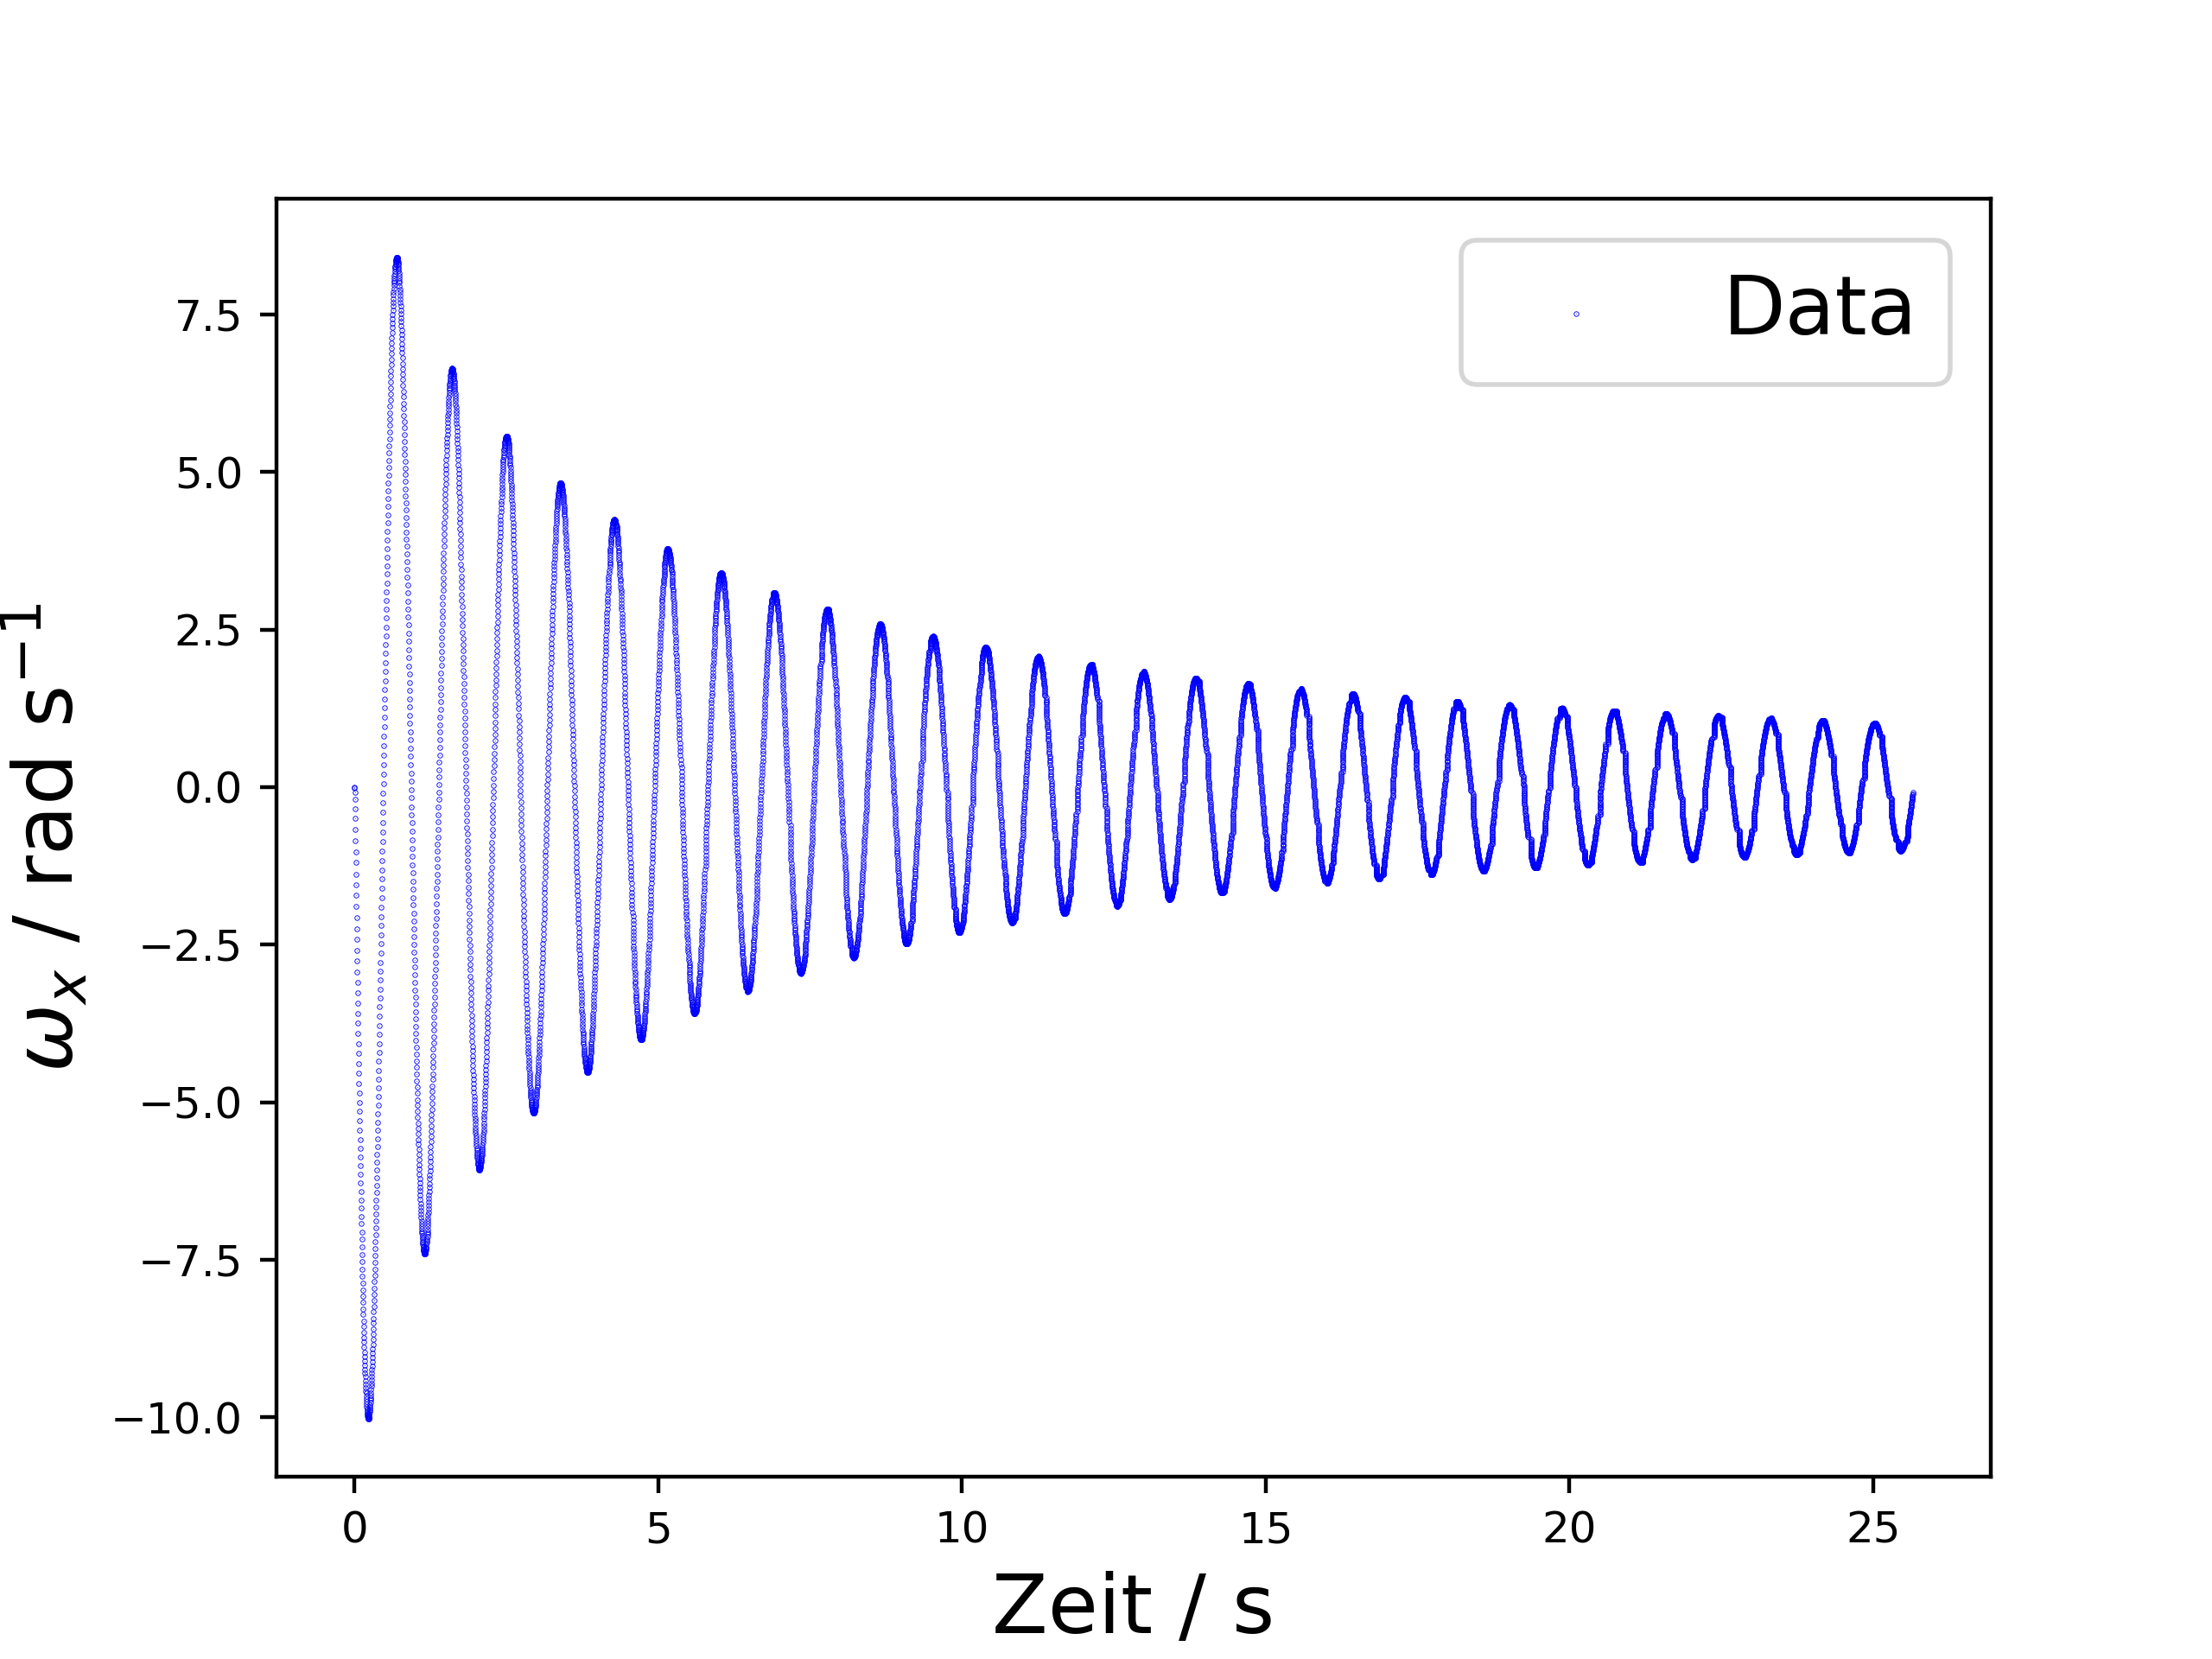
\includegraphics[width=\linewidth]{pics/omega/fit_of_t_wx_mess_nr_4.png}
        \end{minipage}
        \begin{minipage}[htbp]{.32\linewidth} % [b] => Ausrichtung an \caption
            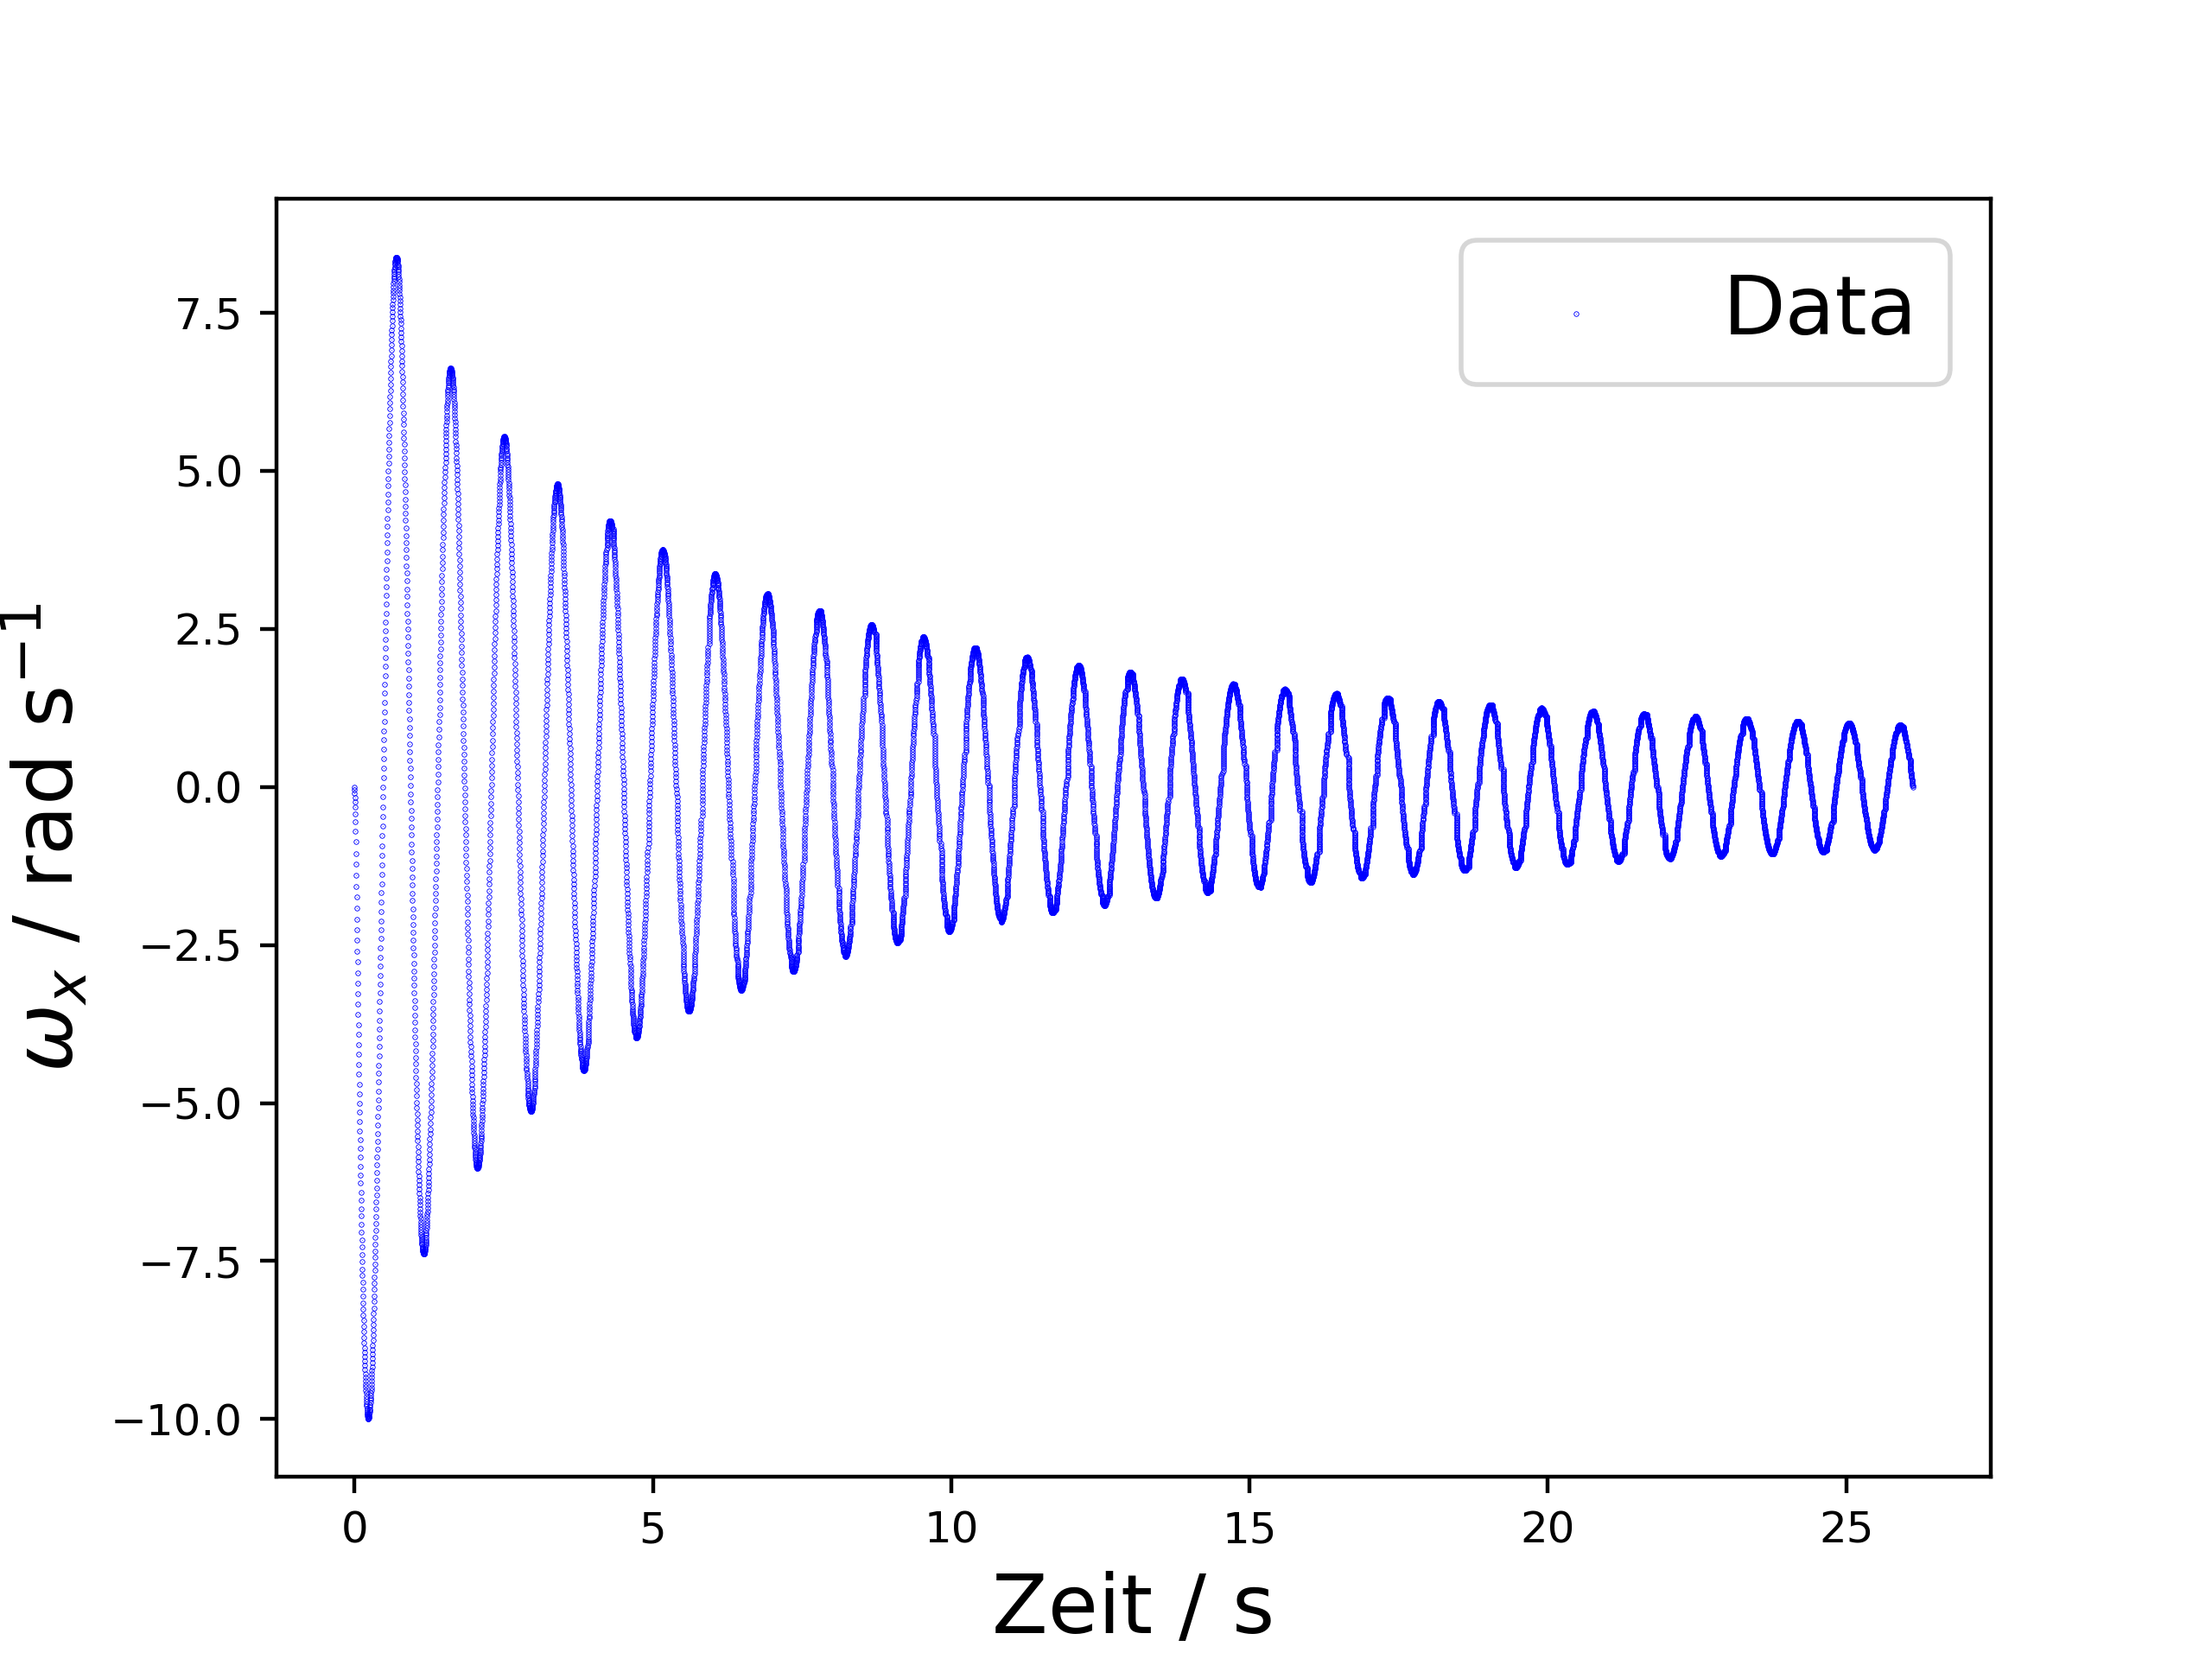
\includegraphics[width=\linewidth]{pics/omega/fit_of_t_wx_mess_nr_5.png}
        \end{minipage}
        \begin{minipage}[htbp]{.32\linewidth} % [b] => Ausrichtung an \caption
            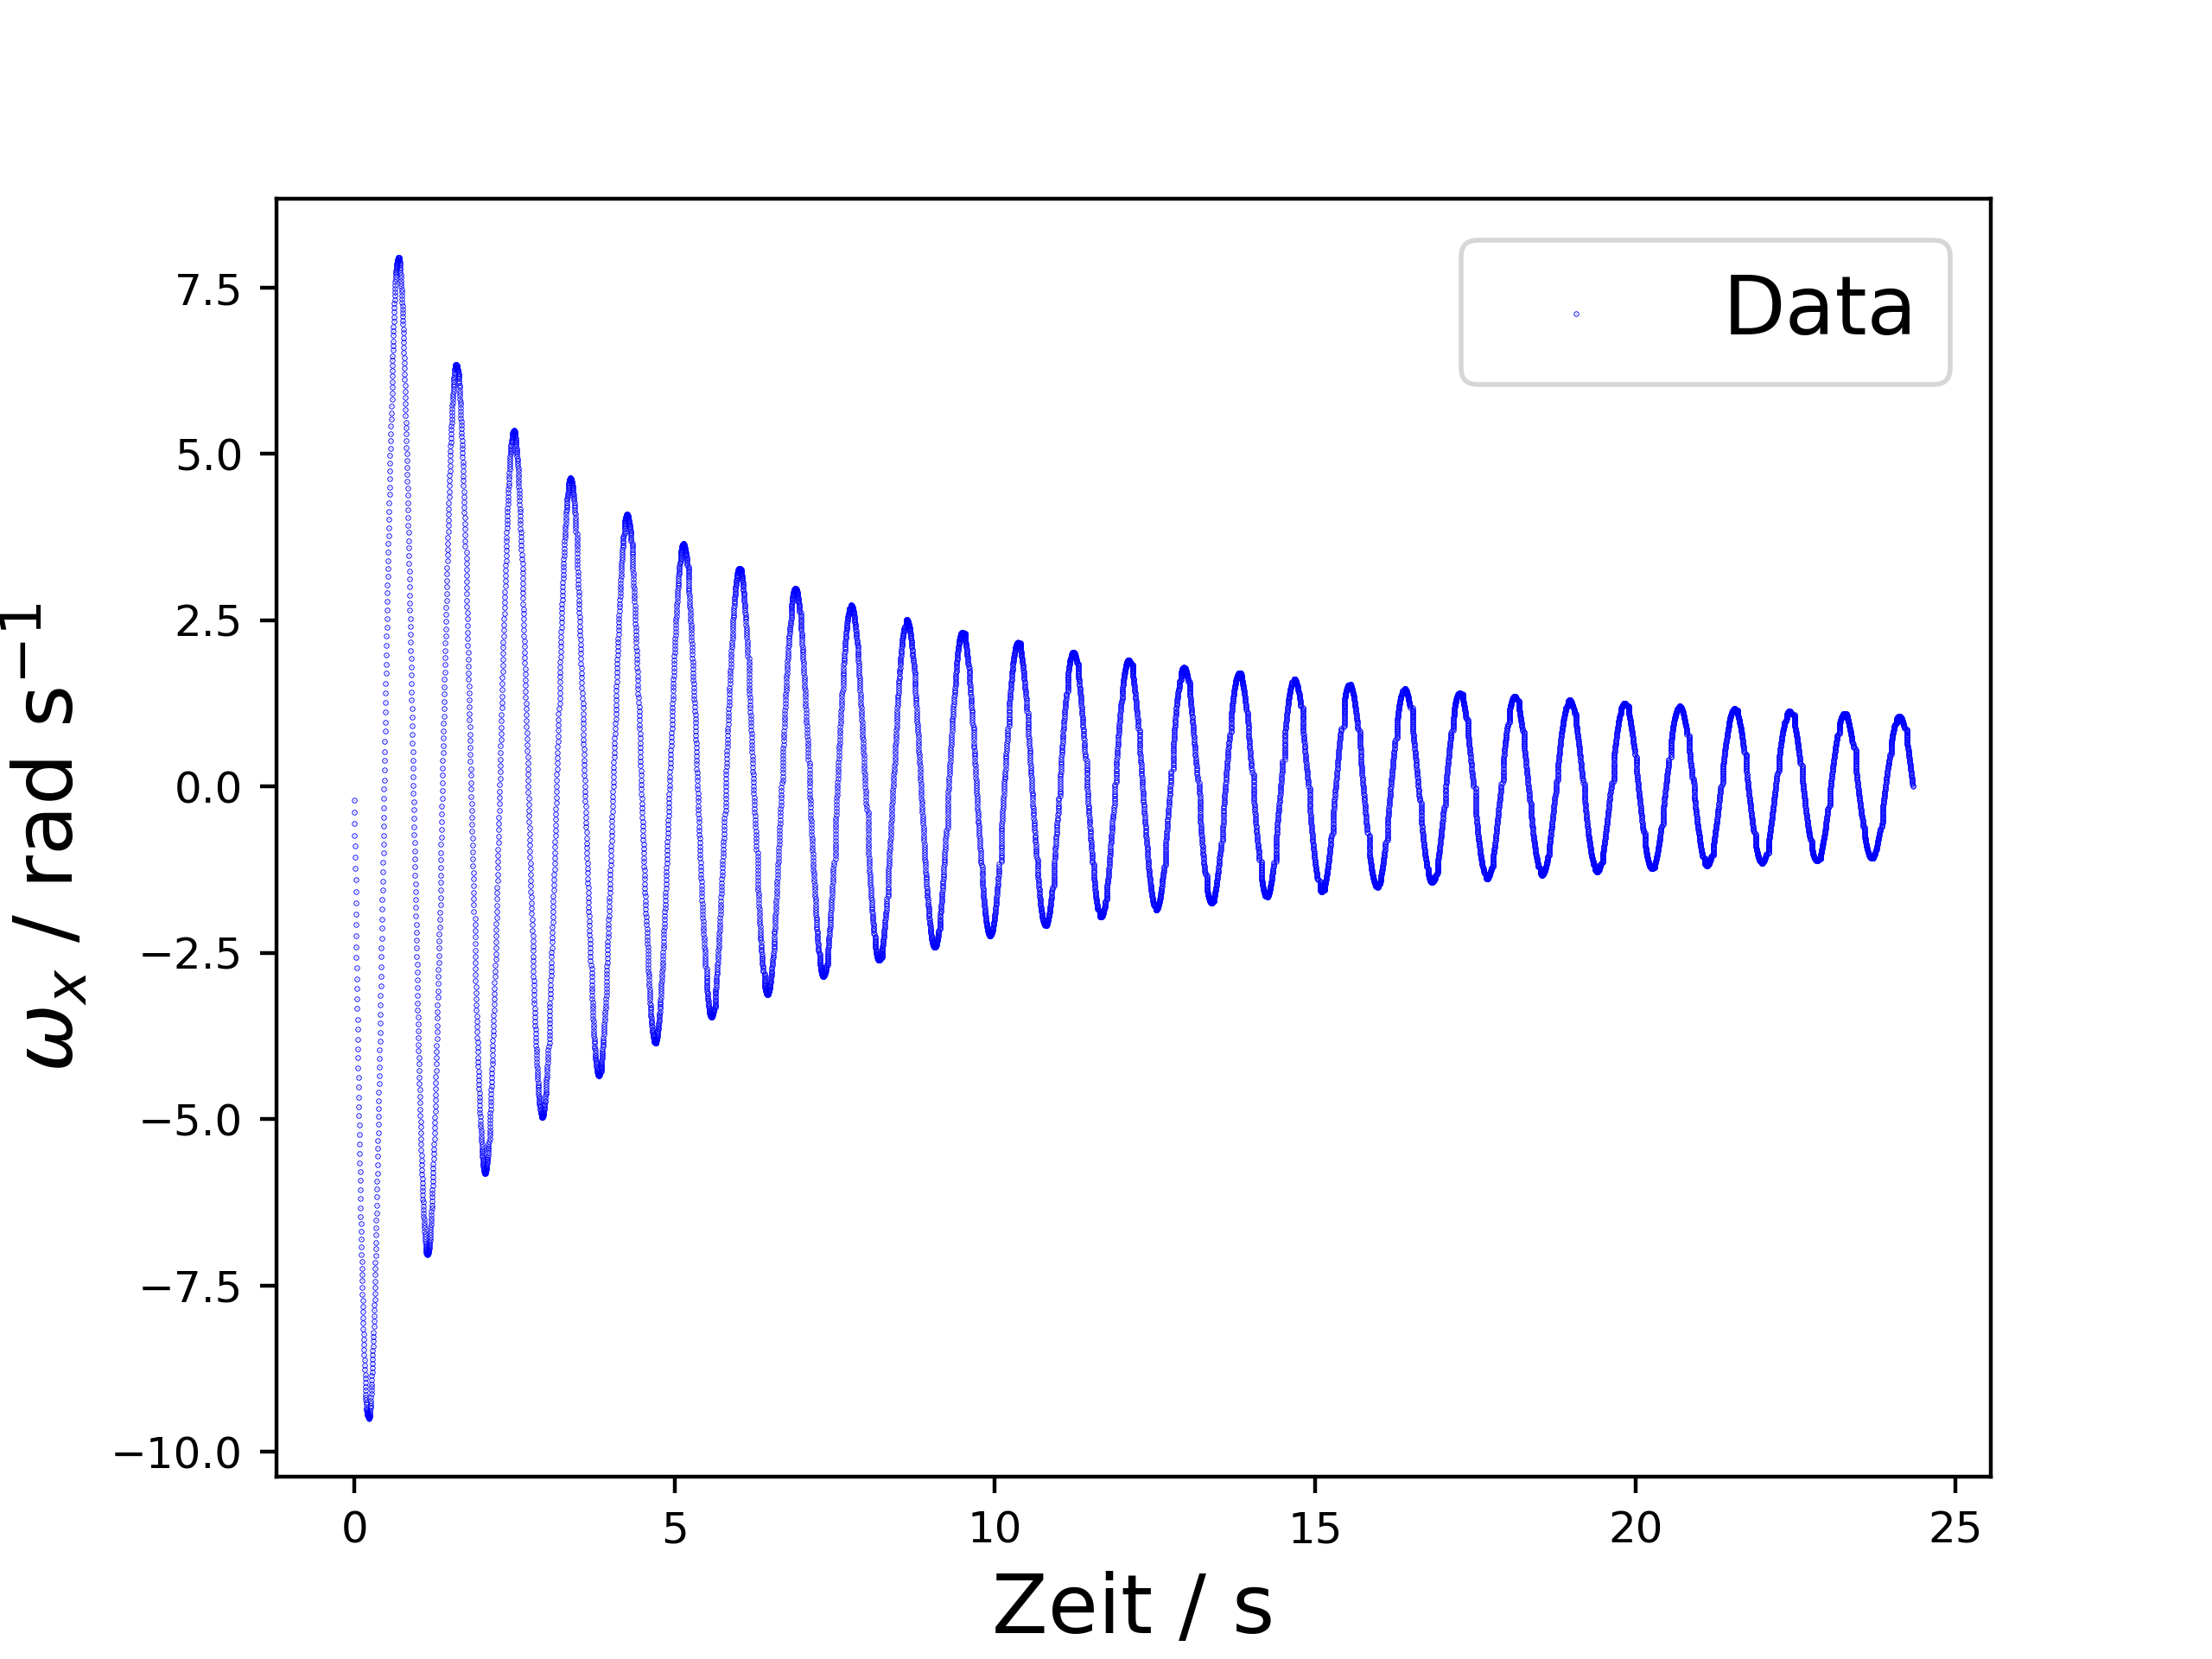
\includegraphics[width=\linewidth]{pics/omega/fit_of_t_wx_mess_nr_6.png}
        \end{minipage}
        \caption[Schwingungsmessungen mit 4 Zusatzgewichte]{3 Messungen der Winkelgeschwindigkeit $\omega_{x}$ in der x-Achse des Smartphones mit 4 Zusatzgewichte.
        Wobei auf der x-Achse die Zeit $t$ / \si{\second} aufgetragen wurde und auf der y-Achse die Winkelgeschwindigkeit $\omega_x$ / \si{\radian\per\second} }

        \label{fig:mit4}
    \end{minipage}
 \end{figure}

\begin{figure}[H]
    \centering
    \begin{minipage}[htbp]{\linewidth}
        \begin{minipage}[htbp]{.32\linewidth} % [b] => Ausrichtung an \caption
            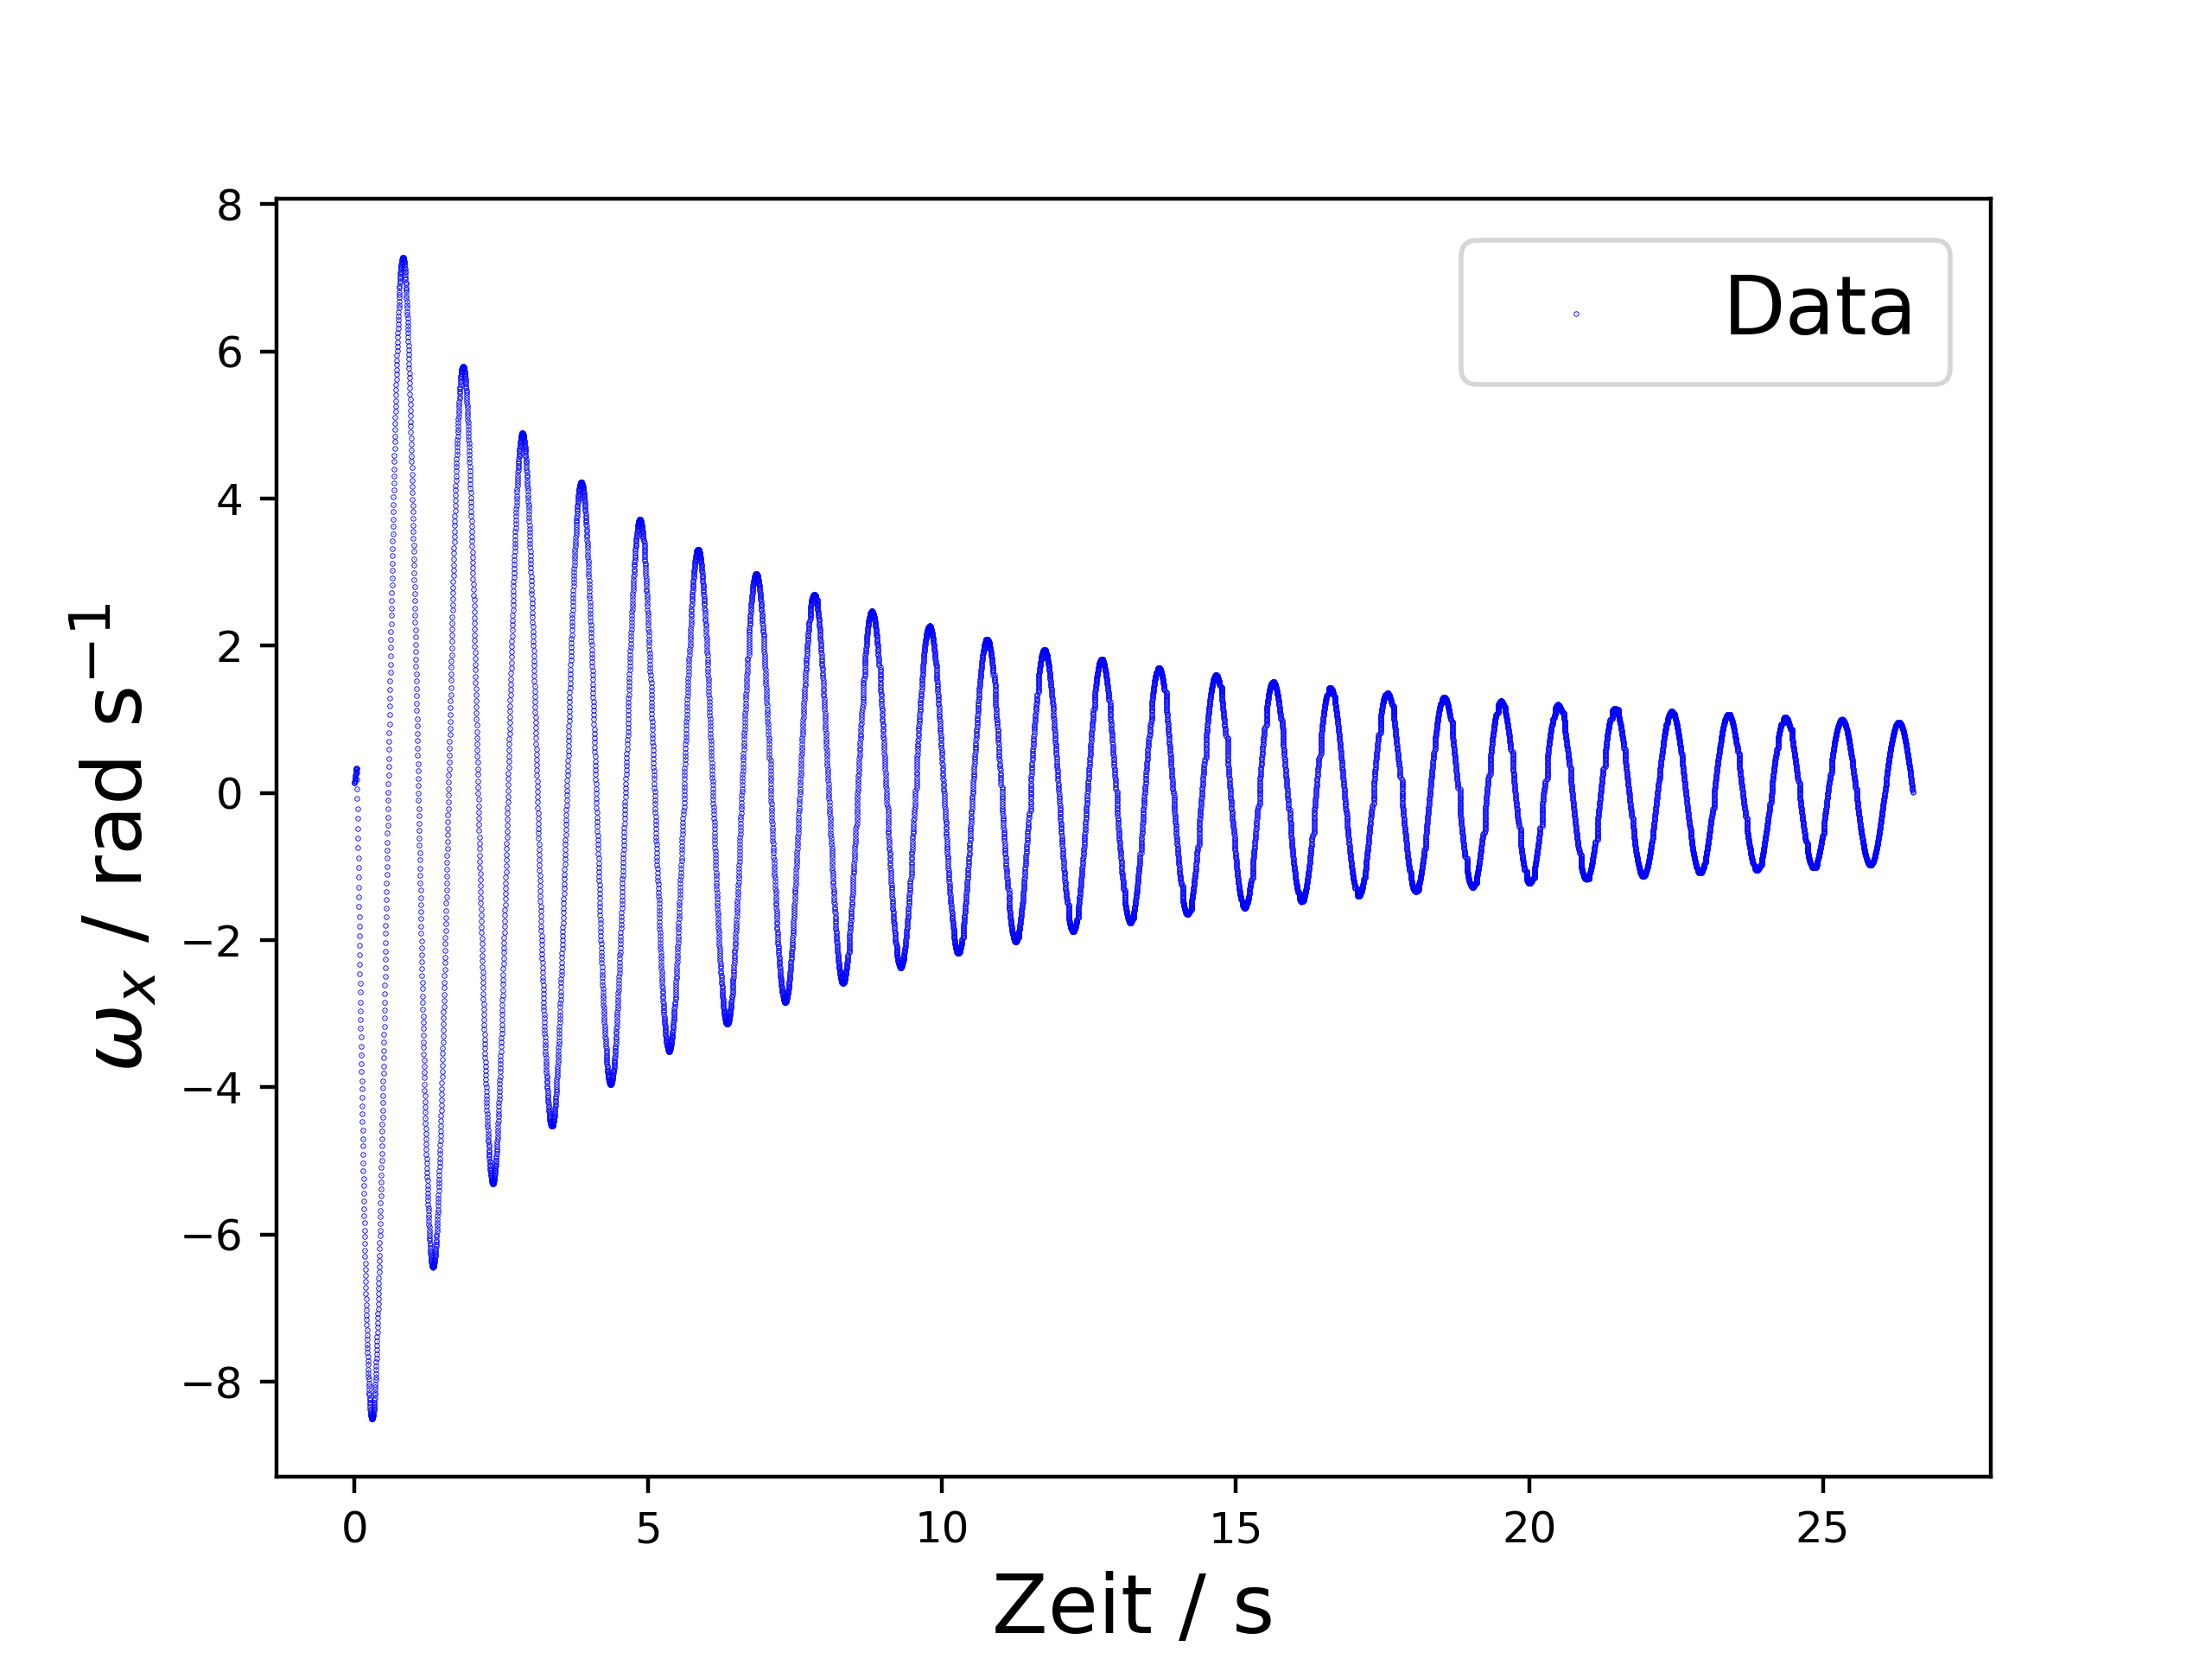
\includegraphics[width=\linewidth]{pics/omega/fit_of_t_wx_mess_nr_7.png}
        \end{minipage}
        \begin{minipage}[htbp]{.32\linewidth} % [b] => Ausrichtung an \caption
            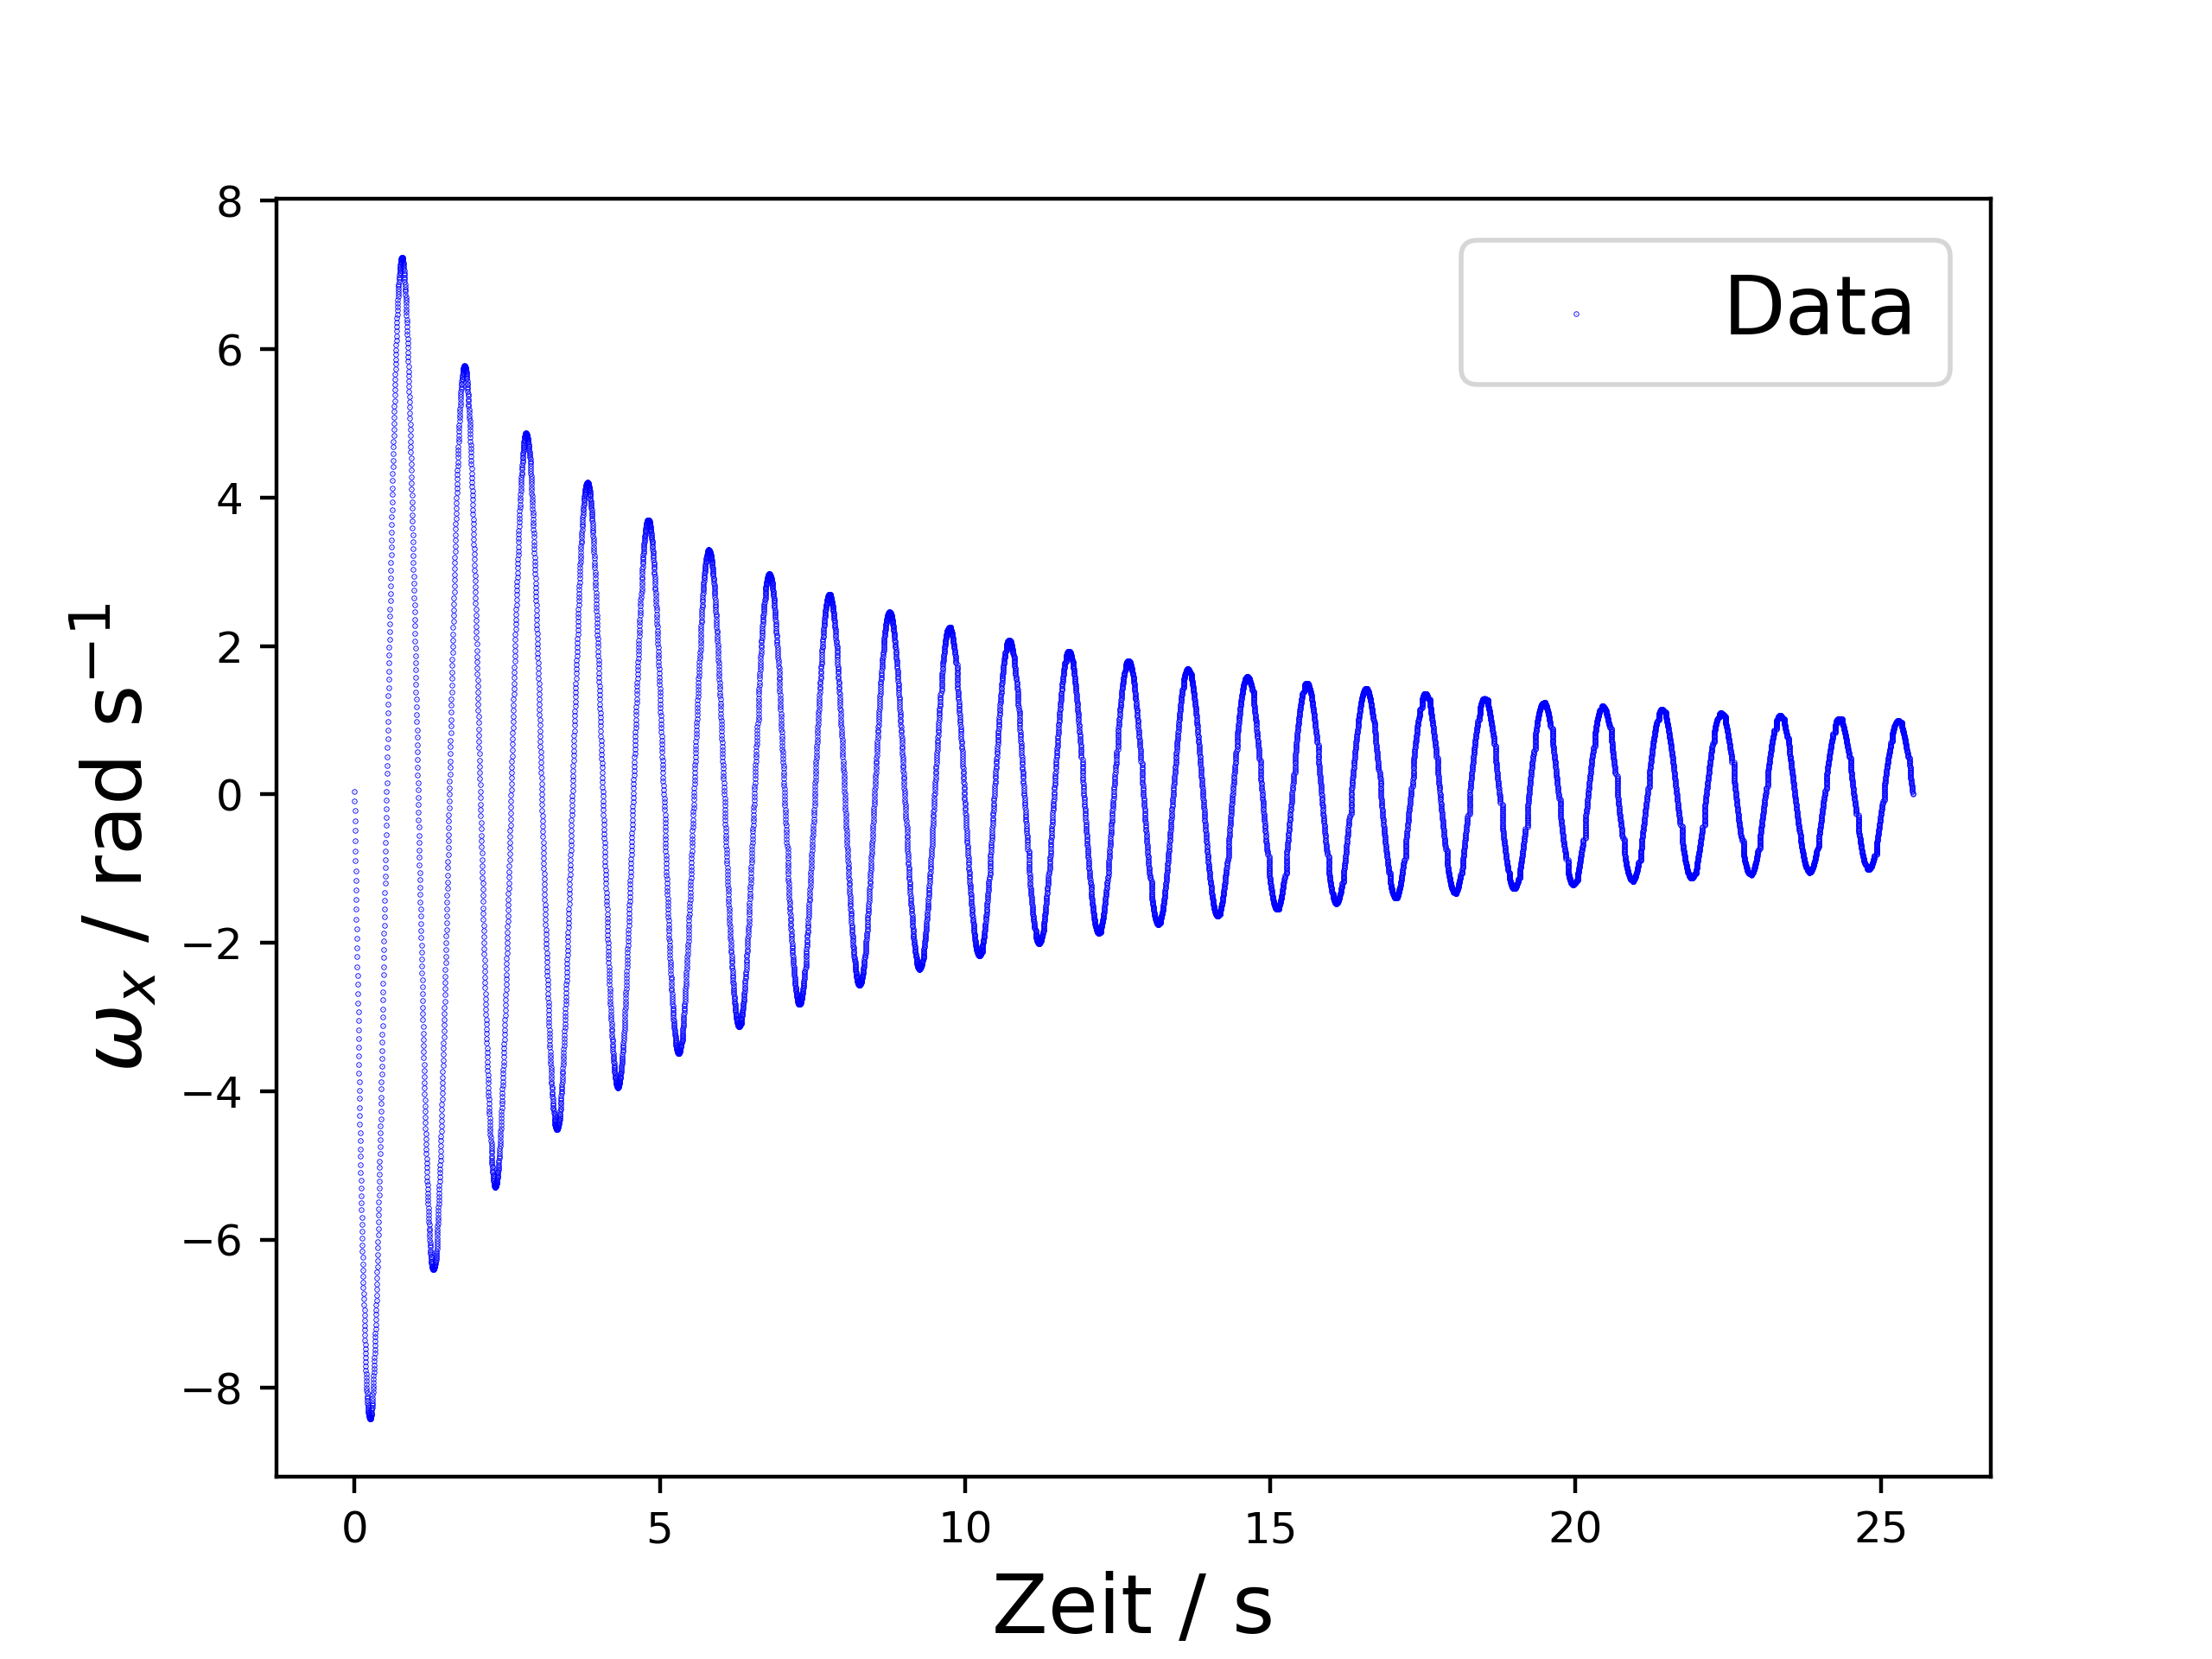
\includegraphics[width=\linewidth]{pics/omega/fit_of_t_wx_mess_nr_8.png}
        \end{minipage}
        \begin{minipage}[htbp]{.32\linewidth} % [b] => Ausrichtung an \caption
            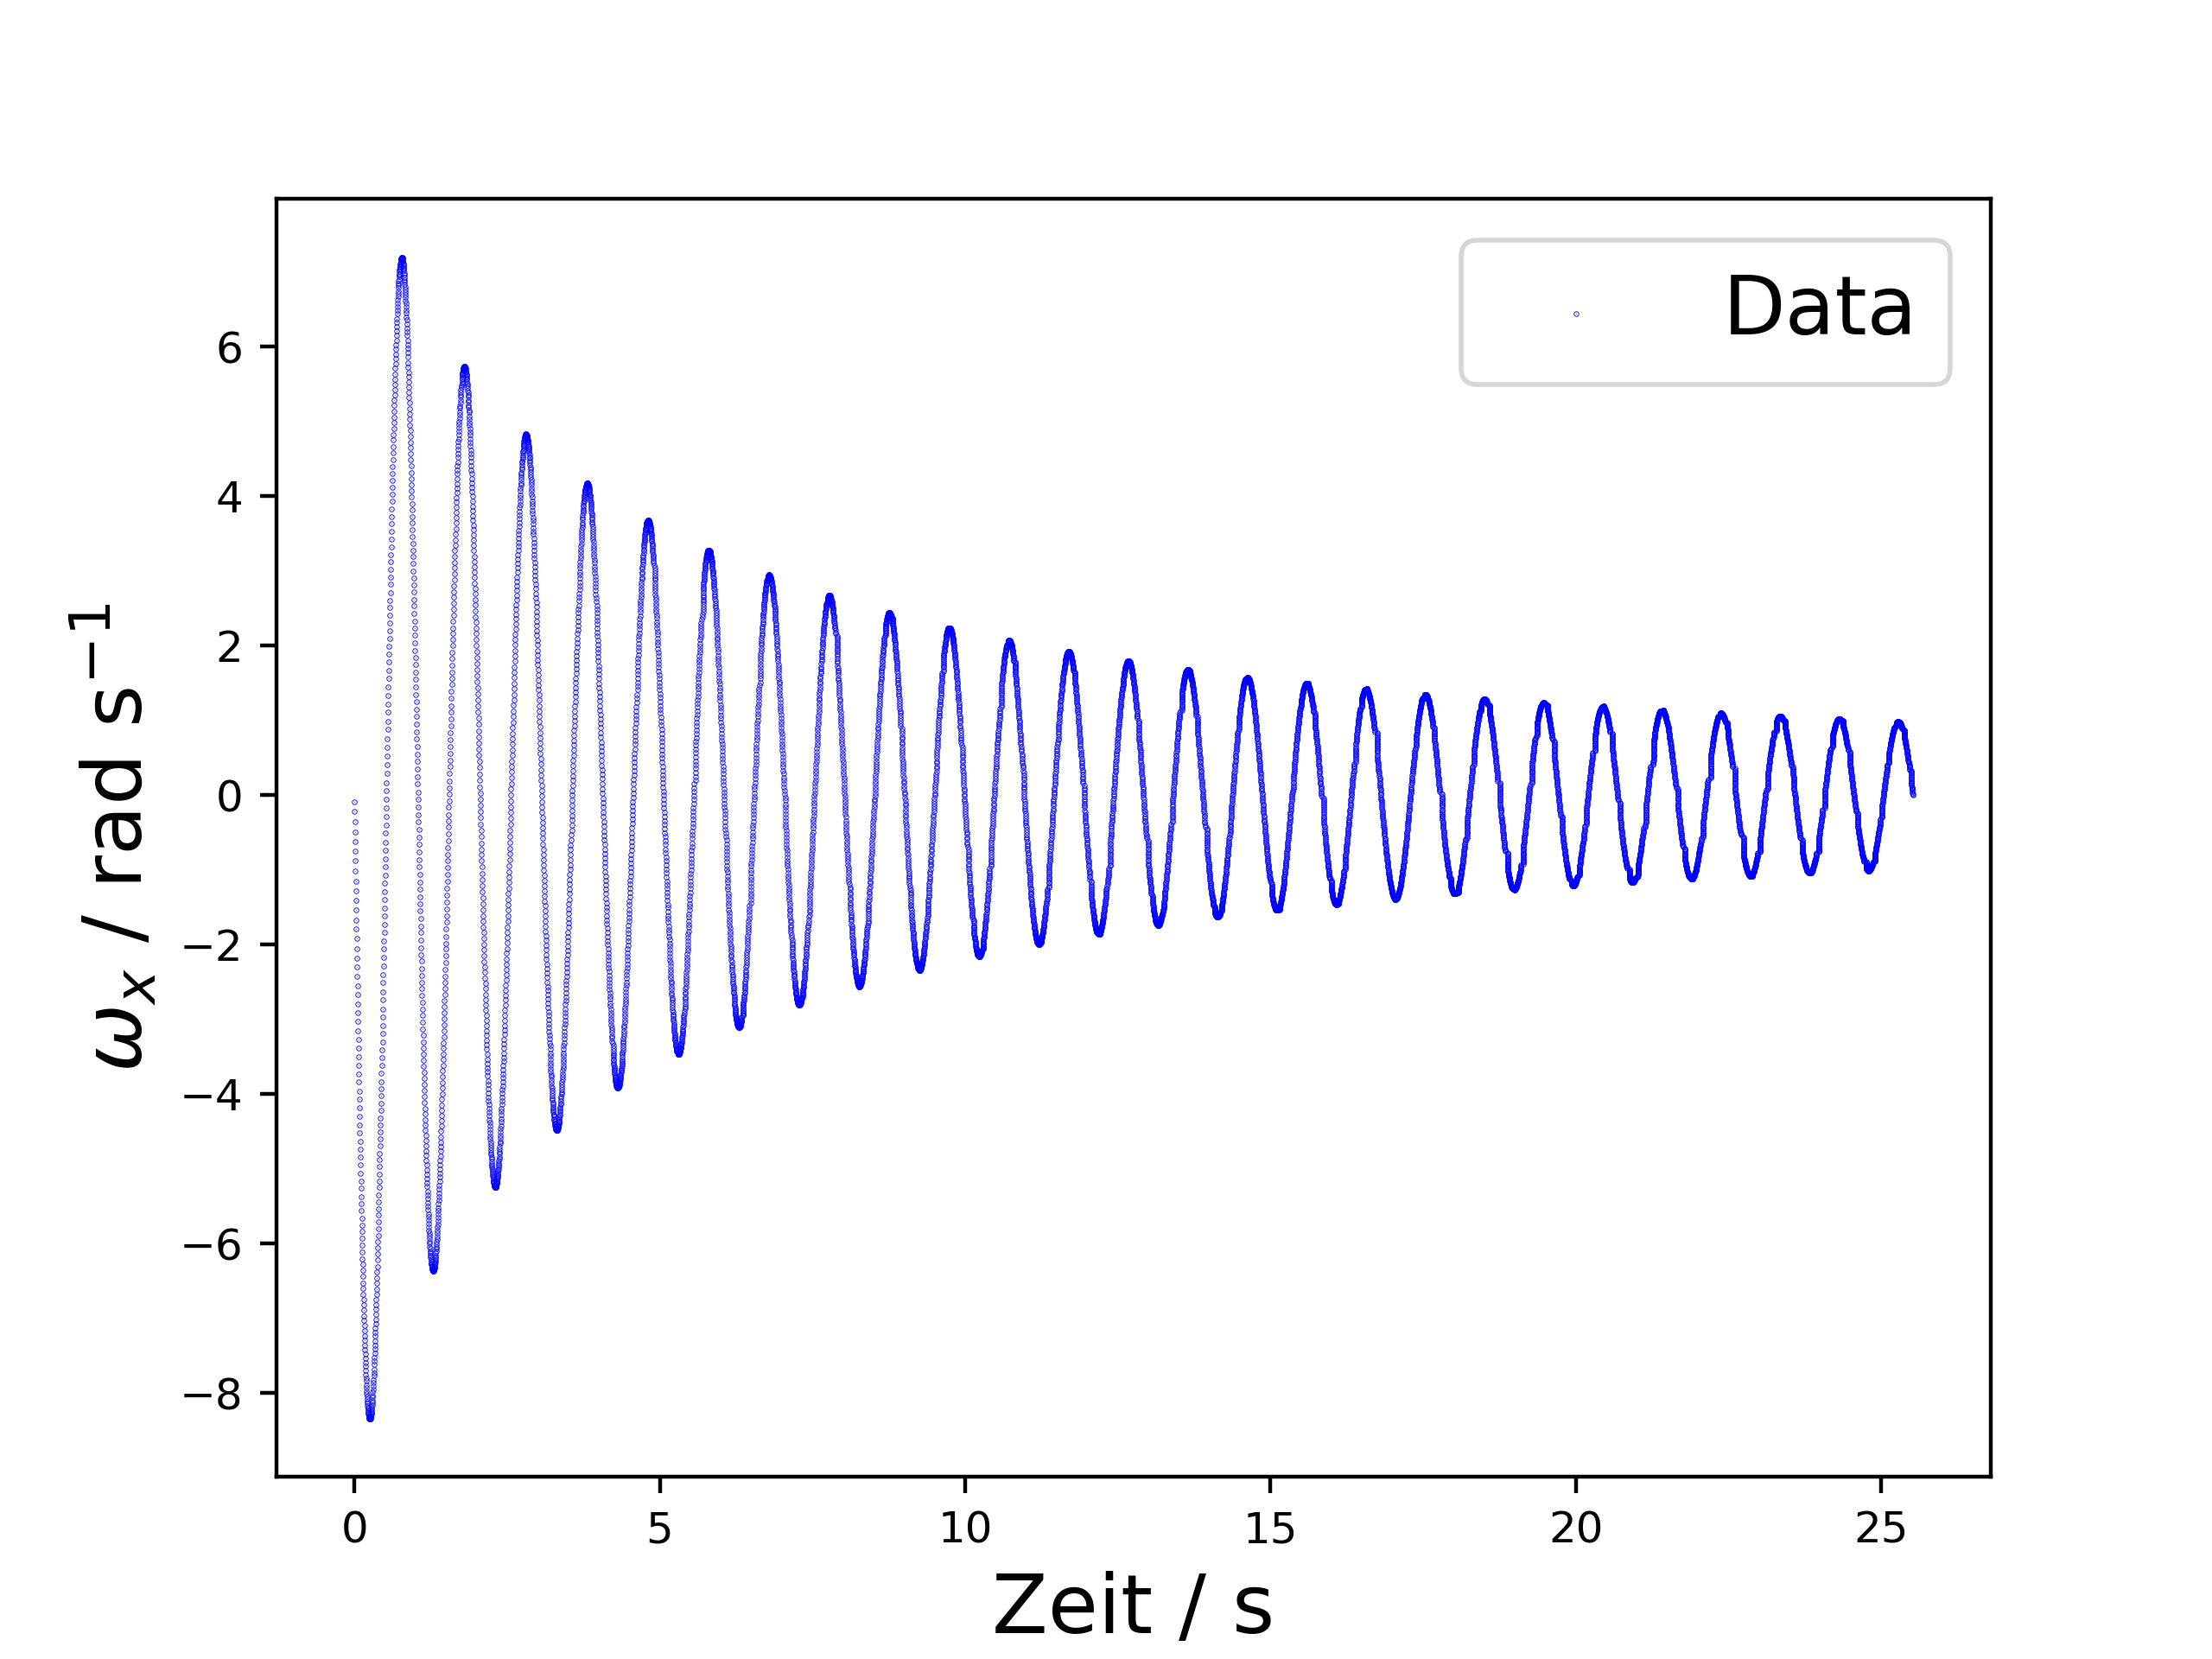
\includegraphics[width=\linewidth]{pics/omega/fit_of_t_wx_mess_nr_9.png}
        \end{minipage}
        \caption[Schwingungsmessungen mit 8 Zusatzgewichte]{3 Messungen der Winkelgeschwindigkeit $\omega_{x}$ in der x-Achse des Smartphones mit 8 Zusatzgewichte.
        Wobei auf der x-Achse die Zeit $t$ / \si{\second} aufgetragen wurde und auf der y-Achse die Winkelgeschwindigkeit $\omega_x$ / \si{\radian\per\second} }
        \label{fig:mit8}
    \end{minipage}
 \end{figure}

\begin{figure}[H]
    \centering
    \begin{minipage}[htbp]{\linewidth}
        \begin{minipage}[htbp]{.32\linewidth} % [b] => Ausrichtung an \caption
            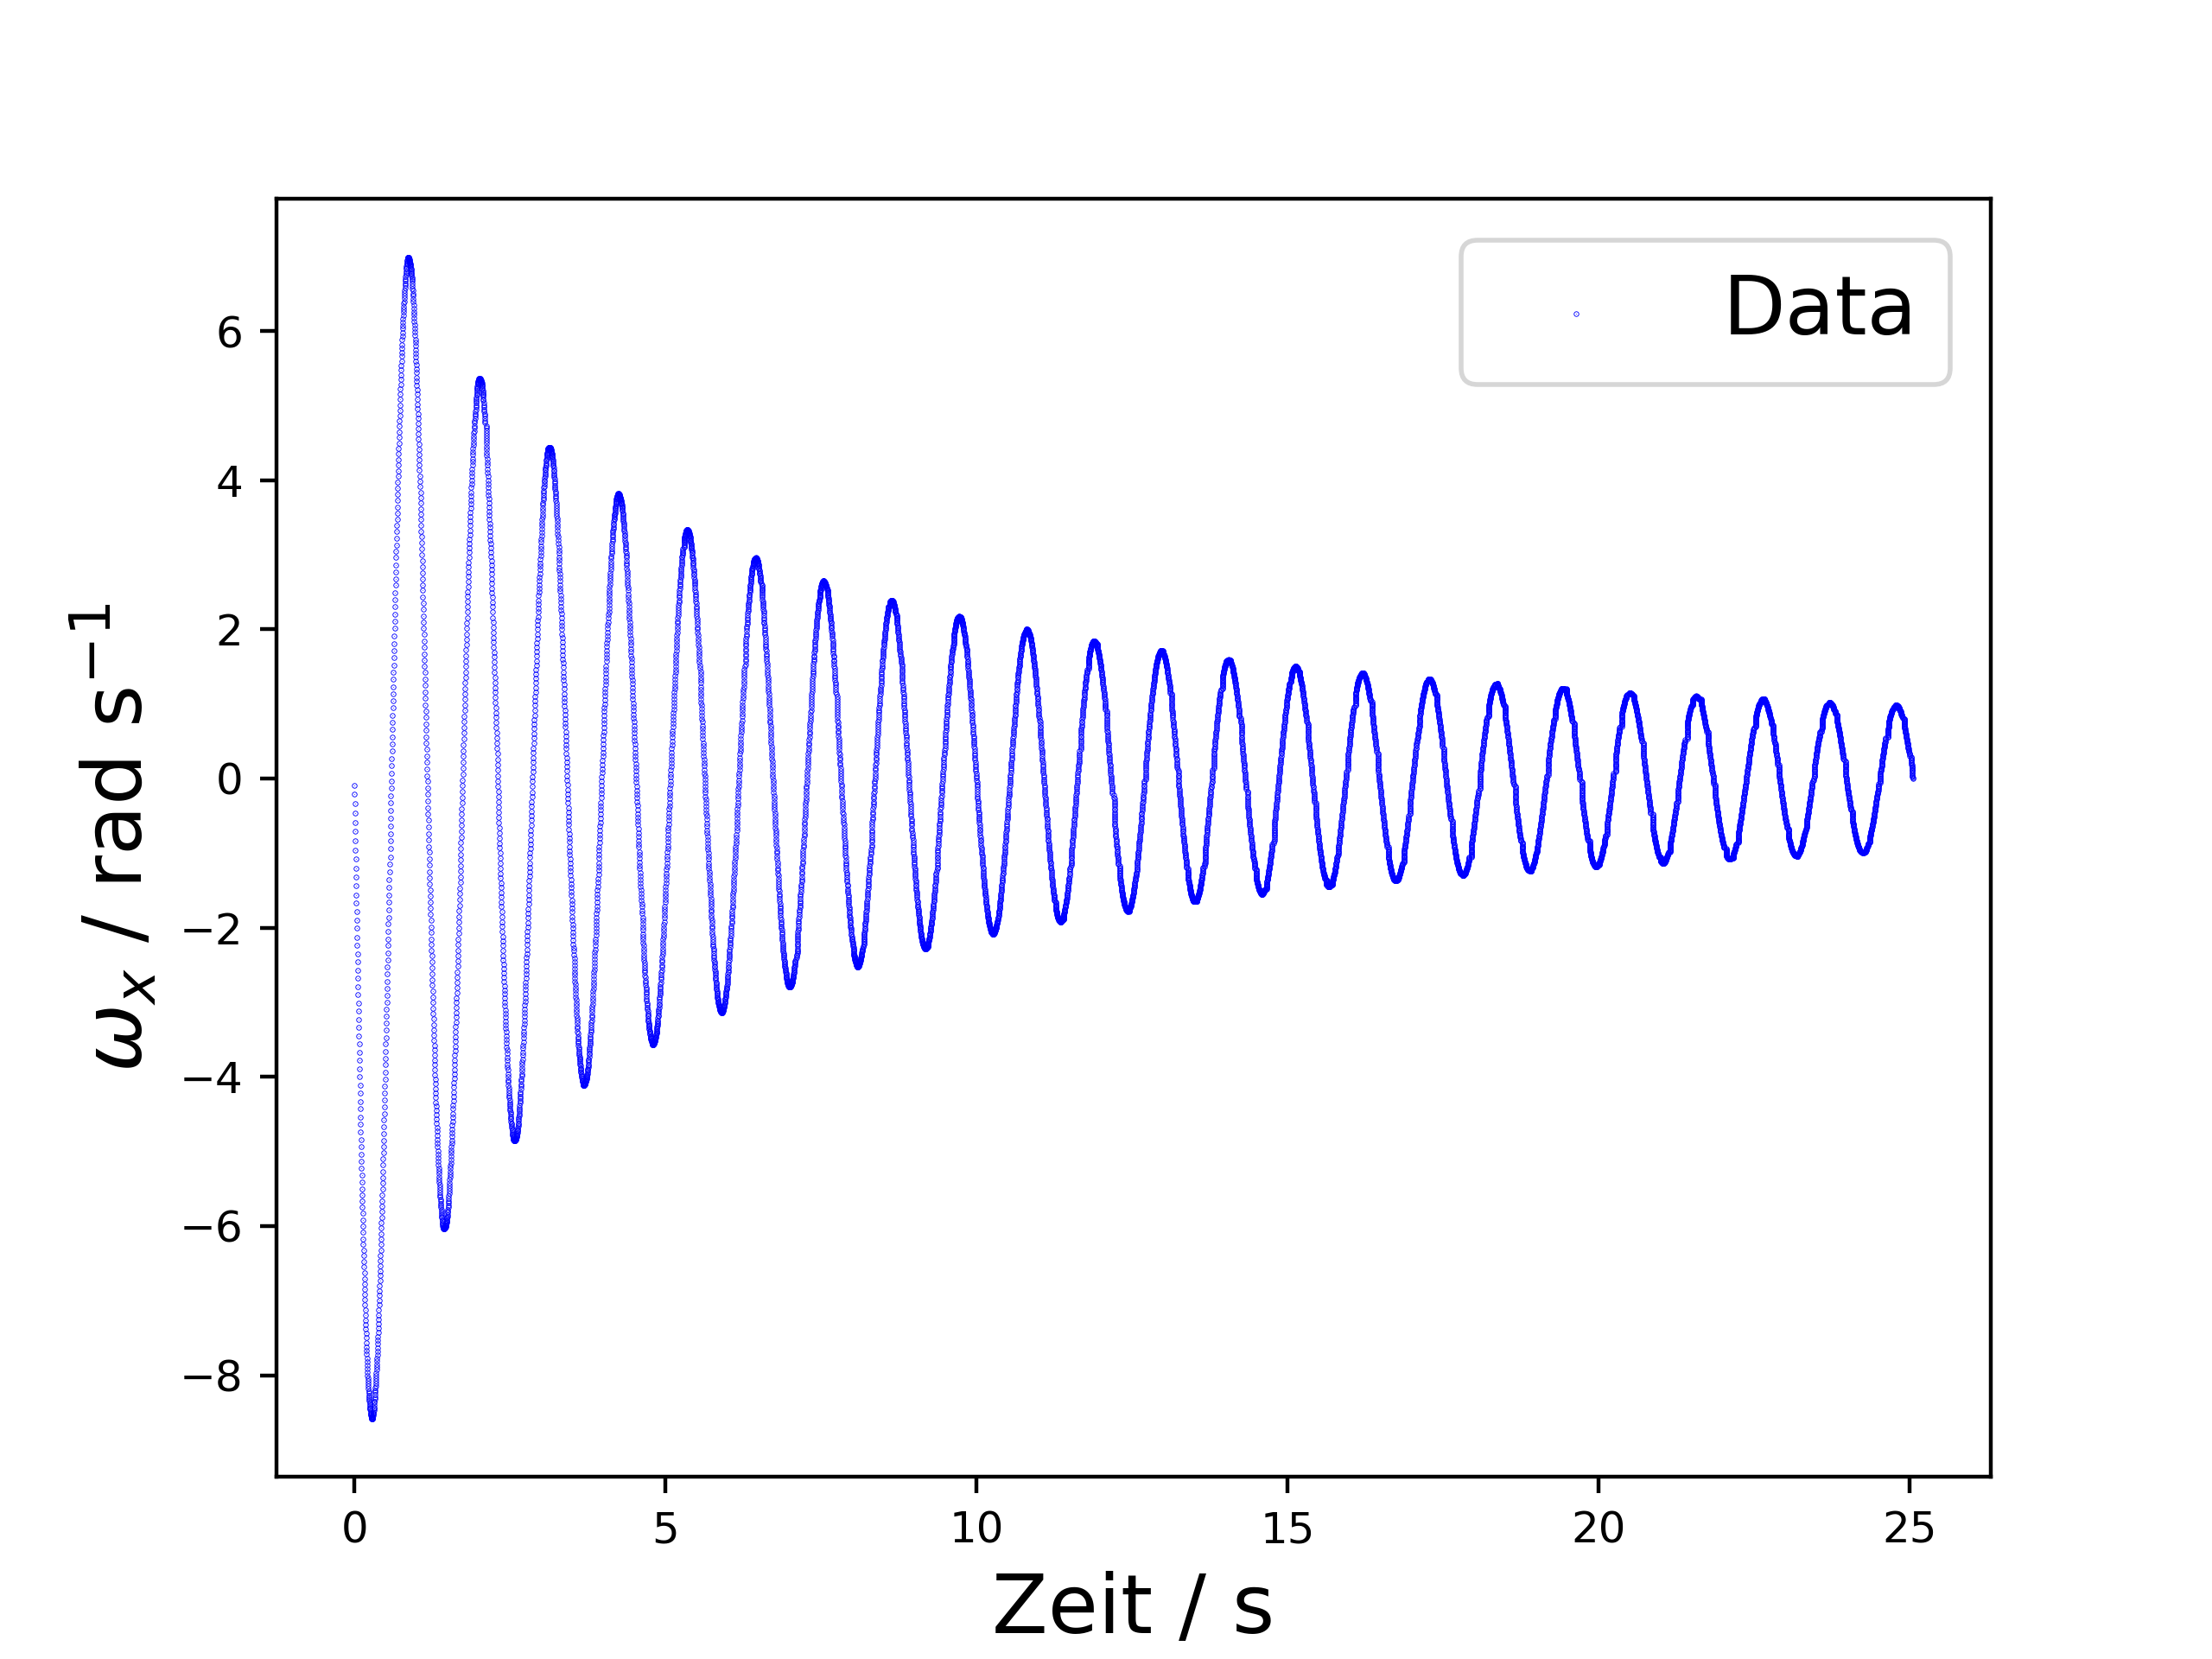
\includegraphics[width=\linewidth]{pics/omega/fit_of_t_wx_mess_nr_10.png}
        \end{minipage}
        \begin{minipage}[htbp]{.32\linewidth} % [b] => Ausrichtung an \caption
            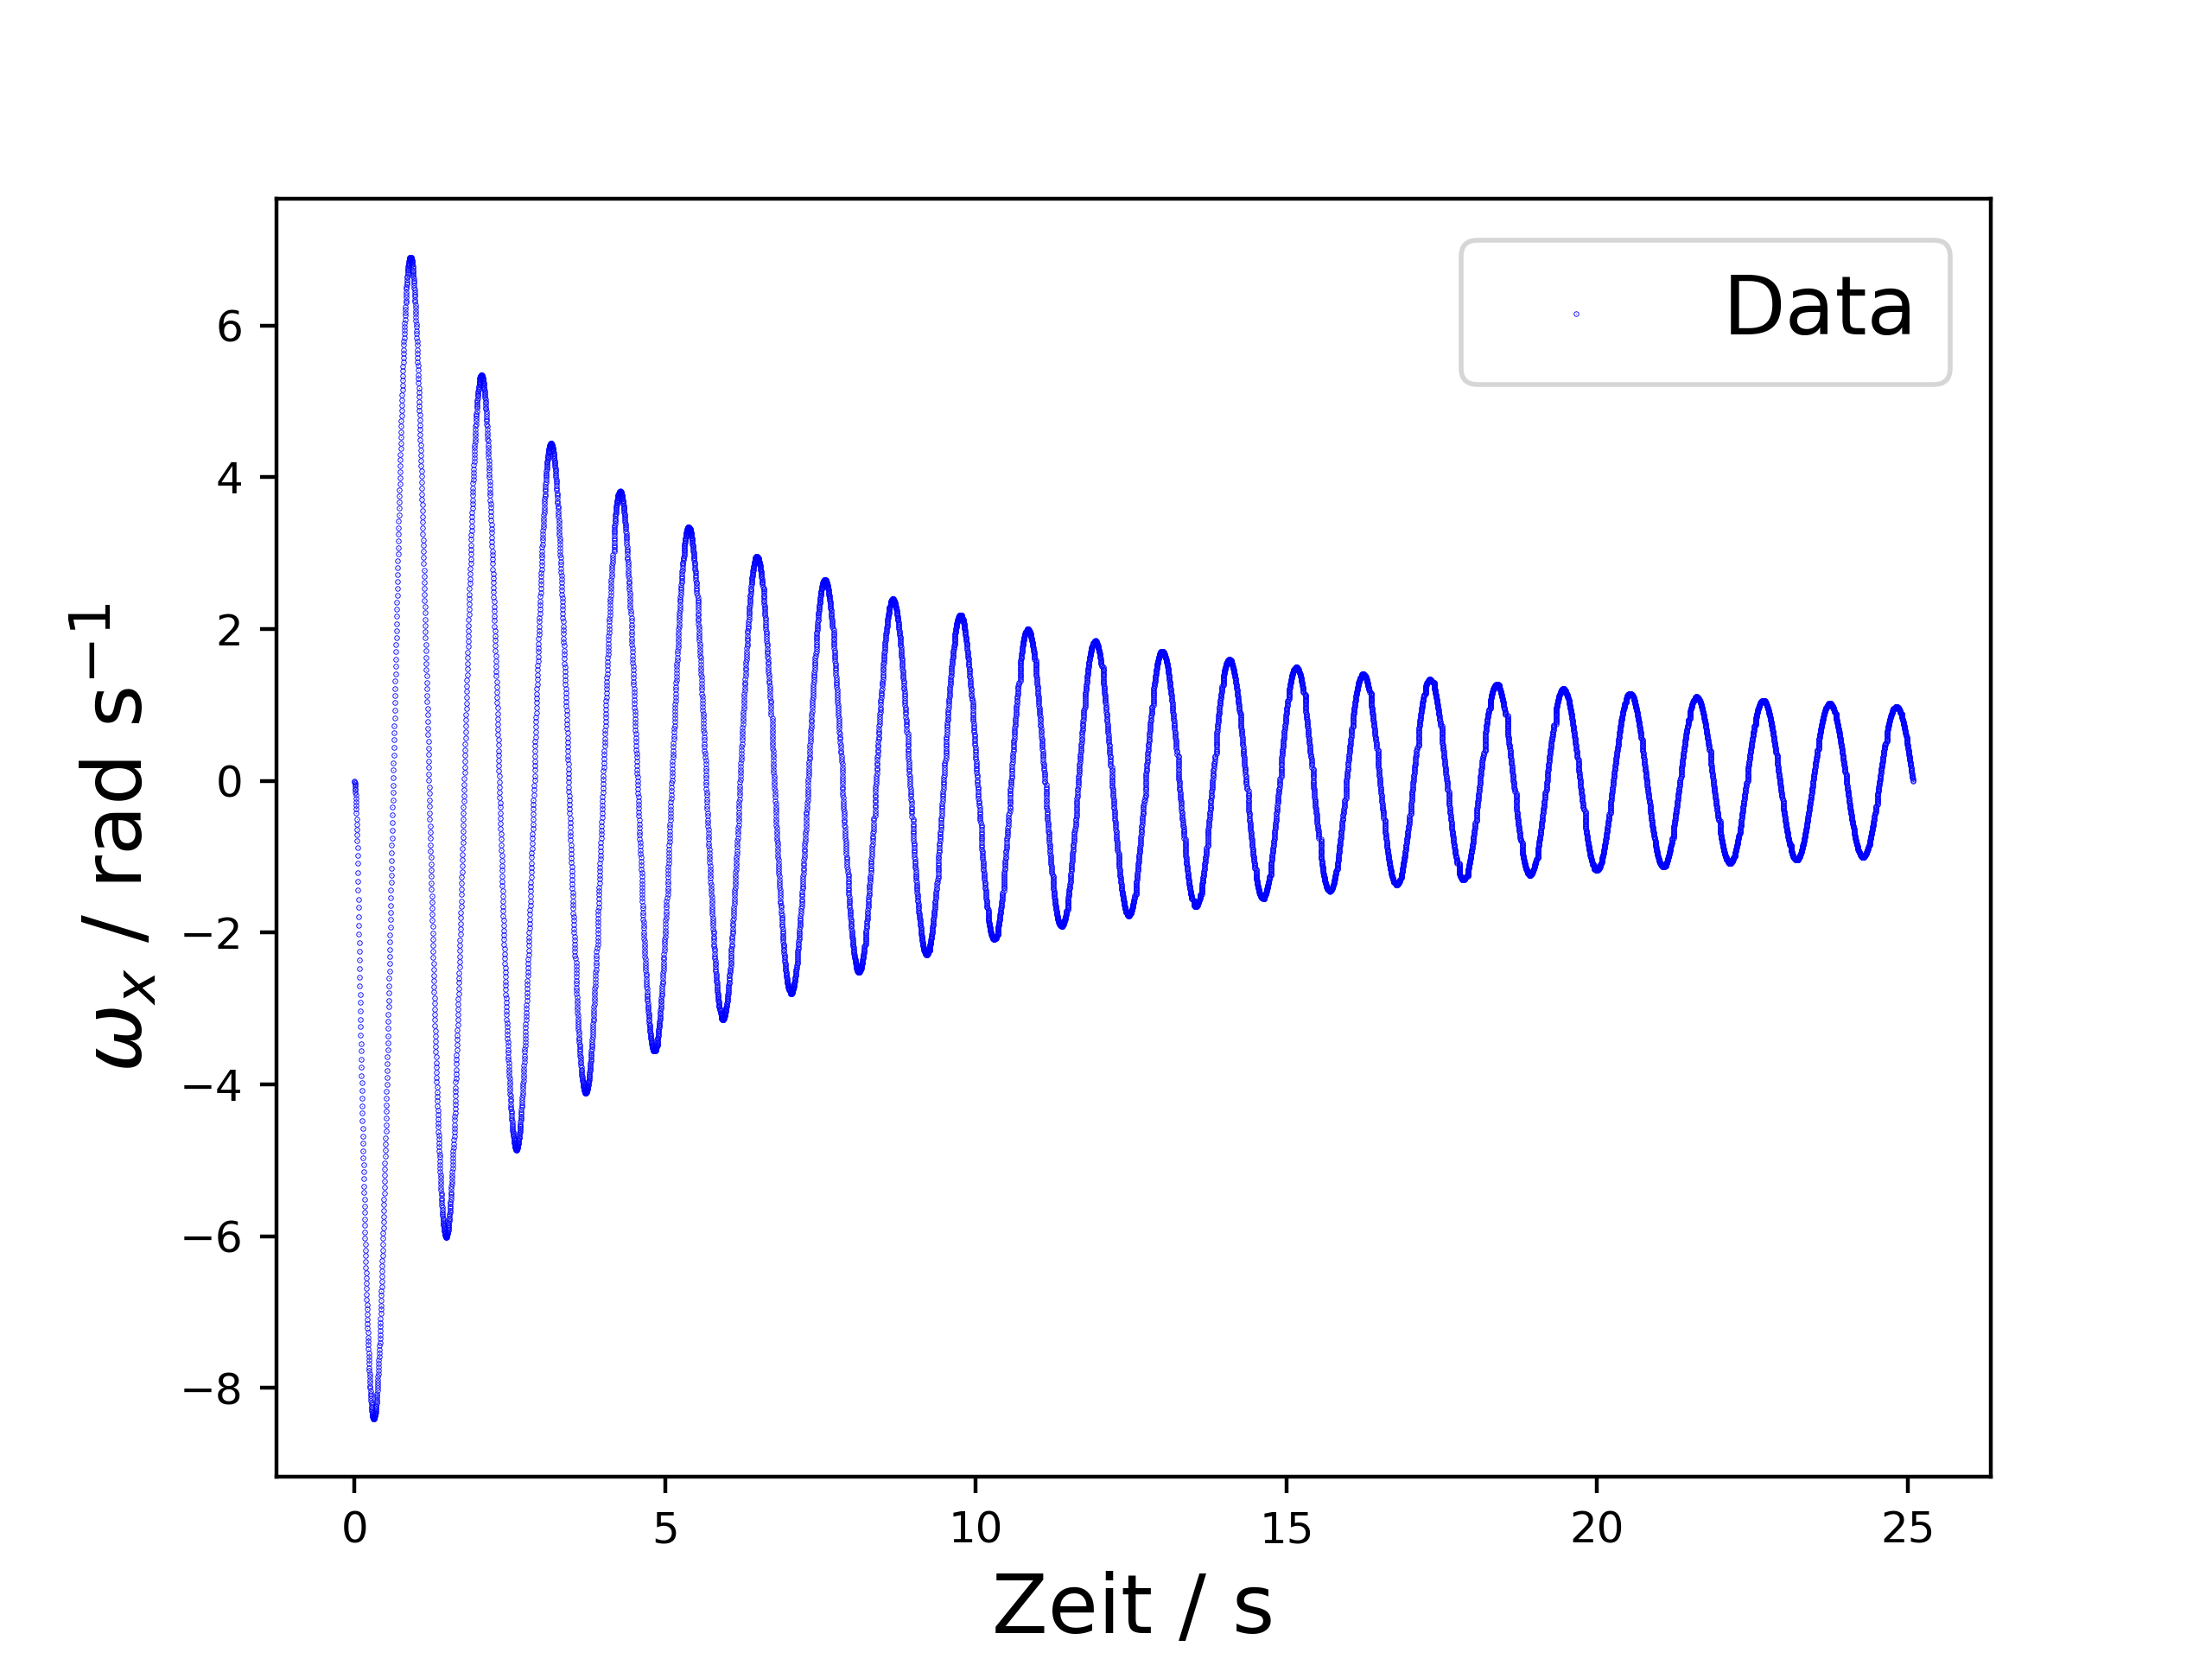
\includegraphics[width=\linewidth]{pics/omega/fit_of_t_wx_mess_nr_11.png}
        \end{minipage}
        \begin{minipage}[htbp]{.32\linewidth} % [b] => Ausrichtung an \caption
            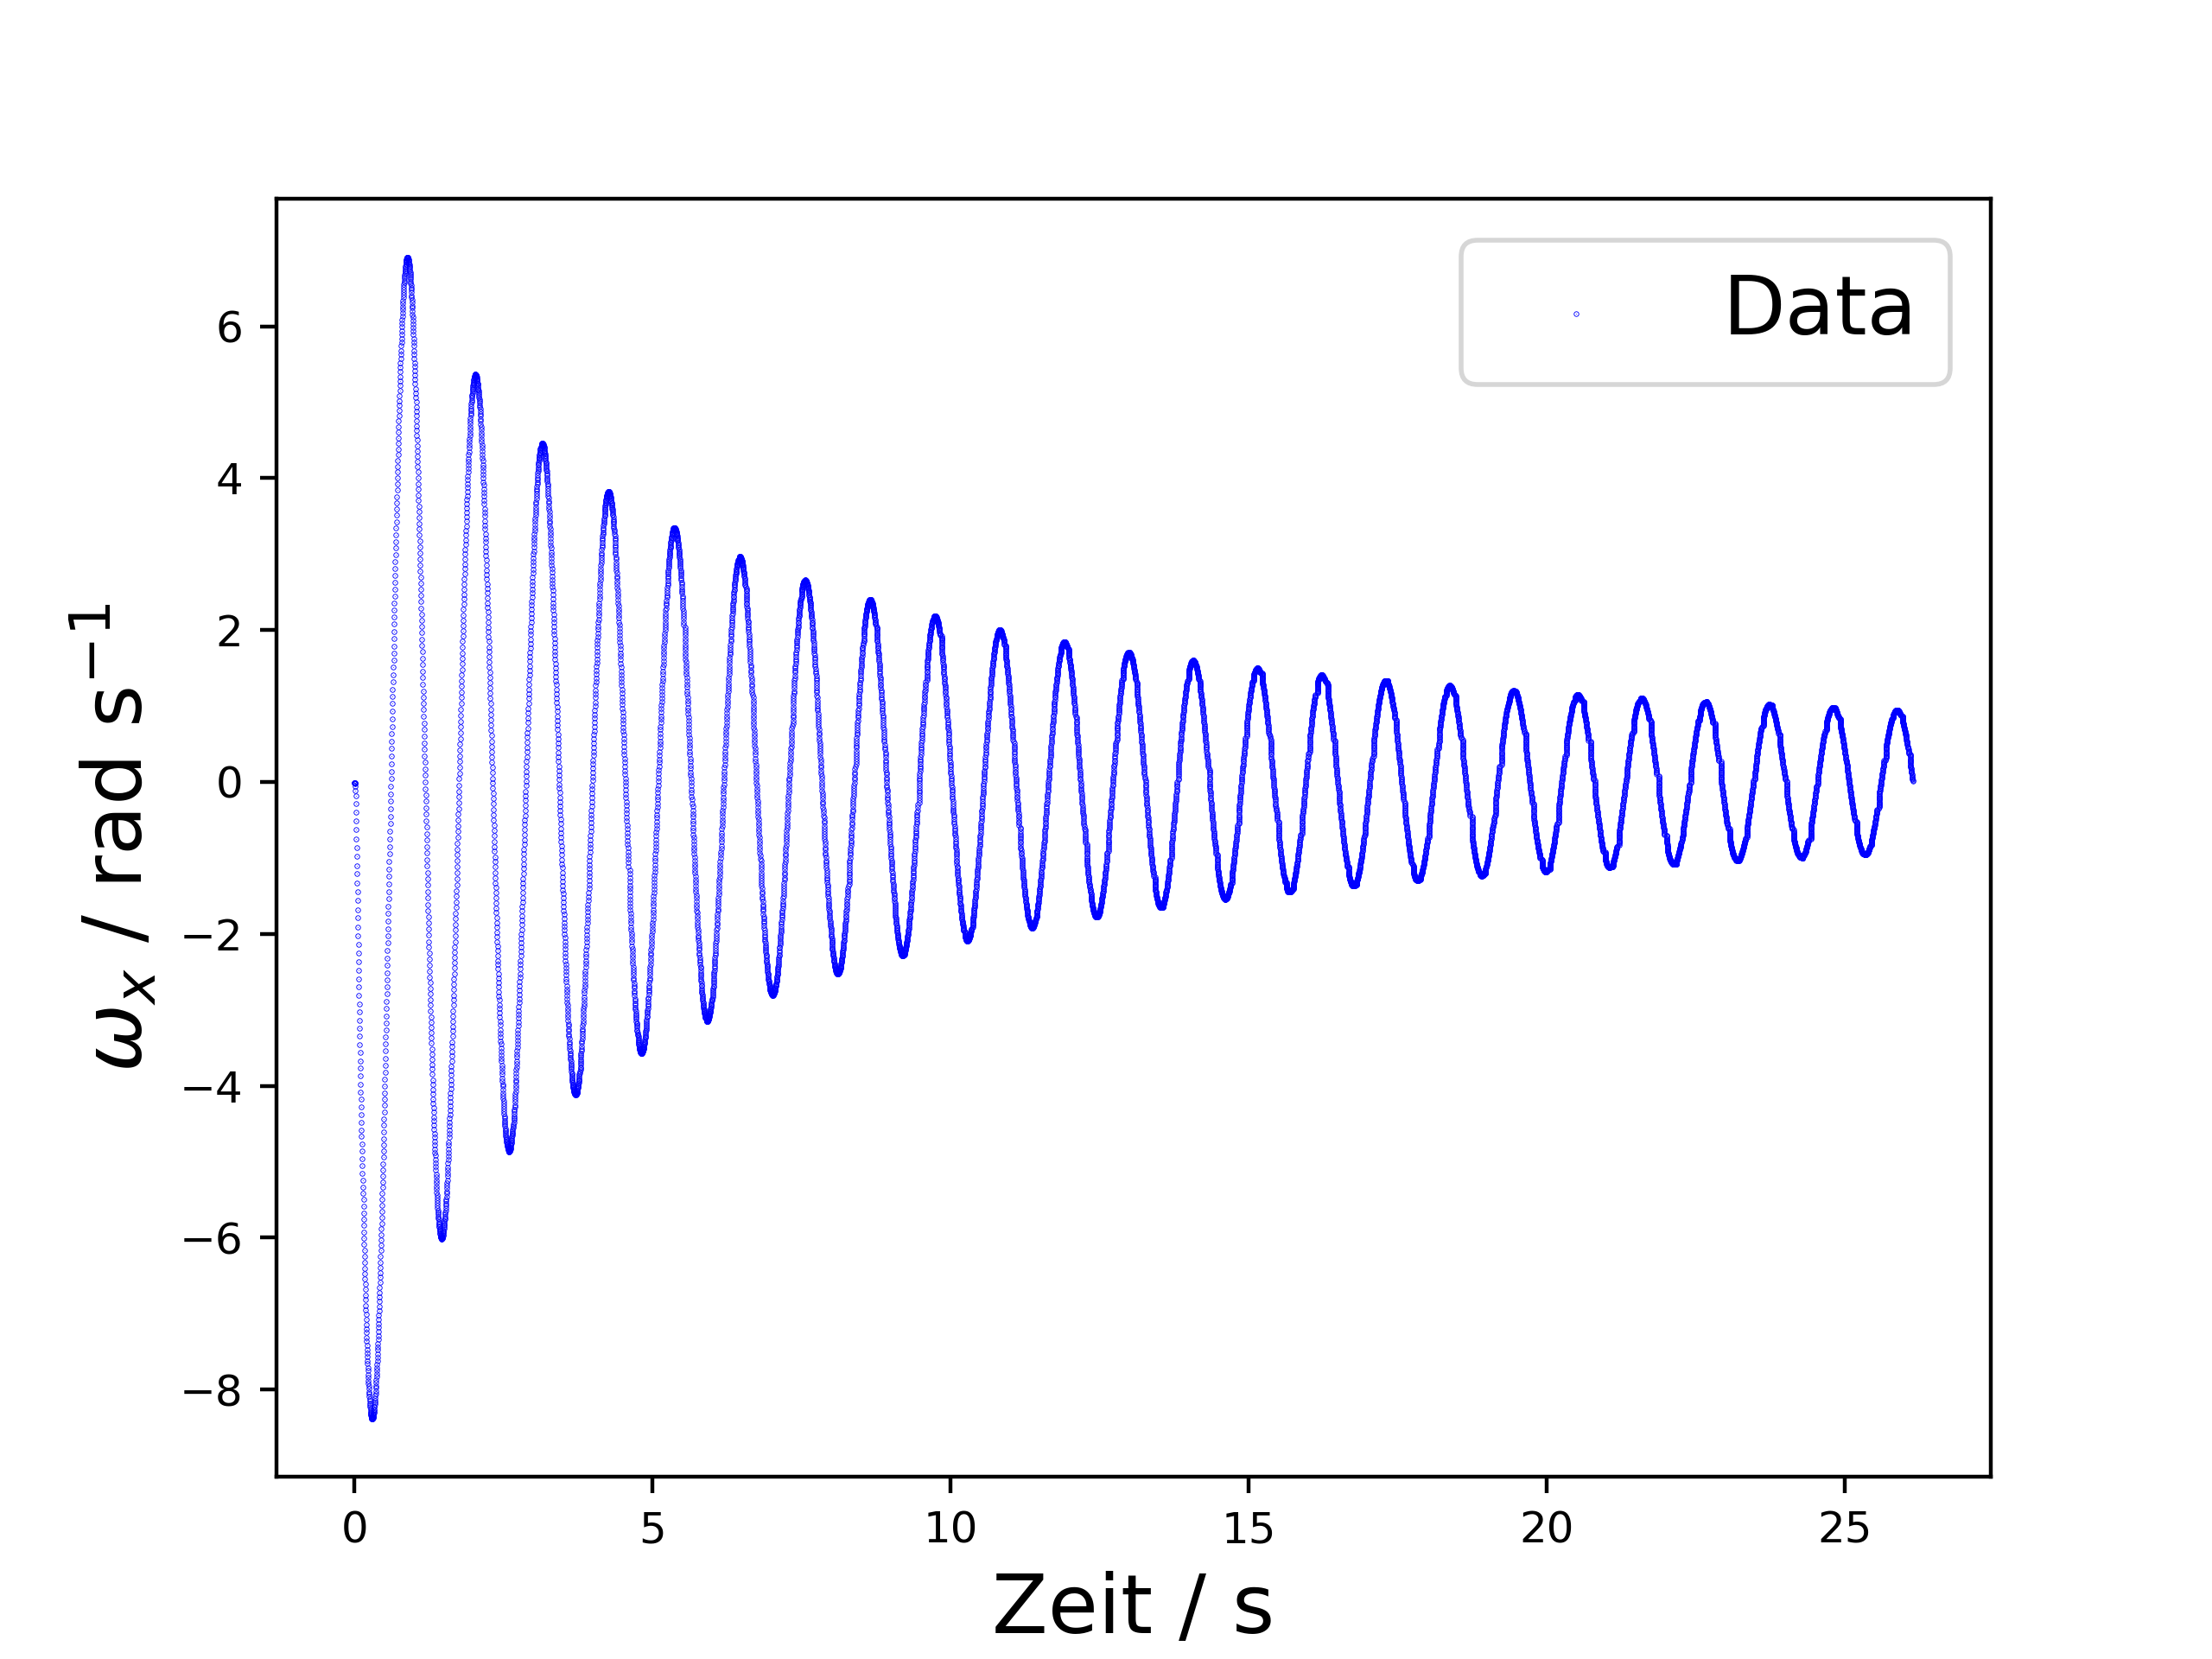
\includegraphics[width=\linewidth]{pics/omega/fit_of_t_wx_mess_nr_12.png}
        \end{minipage}
        \caption[Schwingungsmessungen mit 12 Zusatzgewichte]{3 Messungen der Winkelgeschwindigkeit $\omega_{x}$ in der x-Achse des Smartphones mit 12 Zusatzgewichte.
        Wobei auf der x-Achse die Zeit $t$ / \si{\second} aufgetragen wurde und auf der y-Achse die Winkelgeschwindigkeit $\omega_x$ / \si{\radian\per\second} }
        \label{fig:mit12}
    \end{minipage}
 \end{figure}

Nutz man Python kann man folgende Werte aus den Daten lesen.

\begin{table}[H]
    \centering
    \caption{
        Diese Tabelle beinhaltet alle Relevanten gemessen Werte:\\
        $a$ ist die gemessene Distanze von Drehachse zum Schwerpunkt entlang 
        der Mittelachse, siehe die Skizze \ref{fig:Skizze} \\
        $b$ ist die gemessene Distanze von der halben Dicke des Handys plus Dicke der Münze, siehe die Skizze \ref{fig:Skizze} \\
        $M$ ist das Gewicht einer 50-Cent-Münze \\ 
        $R$ ist der Radius einer 50-Cent-Münze \\
        $|_{10}$ ist das Verhältnis von initialen Auslenkung zur maximalen Auslenkung nach 10 Perioden bei der unbelasteten Schwingung \\
        $t_{10}$ ist die gemessene Zeit von 10 Perioden \\
        $t_{ohne}$ ist die, über alle Perioden gemittelte, Periodendauer der unbelasteten Schwingung \\
        $t_{mit 4}$ ist die, über alle Perioden gemittelte, Periodendauer der mit 4 Münzen belasteten Schwingung \\
        $t_{mit 8}$ ist die, über alle Perioden gemittelte, Periodendauer der mit 8 Münzen belasteten Schwingung \\
        $t_{mit 12}$ ist die, über alle Perioden gemittelte, Periodendauer der mit 12 Münzen belasteten Schwingung \\
    }
    \label{tab:messwerte}
    \begin{tabular}{l|S|S}
        Symbol           & {Wert} & {$\Delta$} \\ \hline
        $a$ / mm         & 66.8     & +-1.7       \\
        $b$ / mm         & 8.35   & +-0.04     \\
        $M$ / g          & 7.80   & 0.005      \\
        $R$ / mm         & 12.125 & 0.003      \\
        $|_{10}$ / \%    & 27     & +-1        \\
        $t_{10}$ / s     & 8.36   & +-0.10     \\
        $t_{ohne}$ / s   & 0.746  & +-0.010    \\
        $t_{mit 4}$ / s  & 0.864  & +-0.018    \\
        $t_{mit 8}$ / s  & 0.975  & +-0.019    \\
        $t_{mit 12}$ / s & 1.07   & +-0.03     \\
    \end{tabular}
\end{table}

Es wurden nur die ersten 10 Perioden genommen um die Dämpfungskonstante 
zu bestimmen, der Grund dafür wird in der \nameref{sec:diskussion_zusammenfassung} besprochen.

\section{Auswertung}
\label{sec:auswertung}

Werden die $a$, $b$, $M$ und $R$ mit der \autoref{eq:zusatzI} kombiniert
bekommt man folgenden Wert für das Trägheitsmoment der Zusatzgewichte $I'$:

\begin{equation}
    I' = \SI{142(8)}{\kg\mm\squared}
\end{equation}

Um nun das Direktionsmoment $D_r$ zu finden werden, die Quadrate der Periodendauern $t_{*}$
in Abhängigkeit der Anzahl an hinzufügten Trägheitsmomenten $n$
geplottet (wie in \autoref{eq:perioden_lin_reg} zusehen ist) und an eine lineare Funktion gefittet.

\begin{figure}[H]
    \centering
    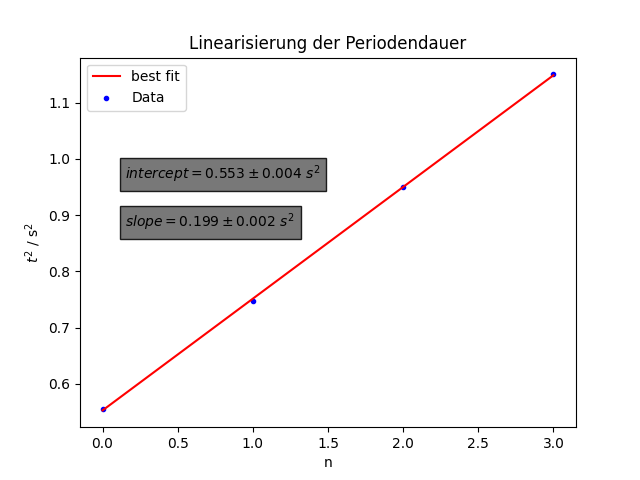
\includegraphics[width=0.8\linewidth]{pics/lin_reg_n_t.png}
    \caption{Das Bild veranschaulicht die lineare Regression der Quadrate Periodendauern $t^2$
    gegenüber der Anzahl an hinzufügten Trägheitsmomenten $n$}%
    \label{fig:lin_reg}
\end{figure}

Durch die Steigung (Slope) $k$ der Geraden ist lässt sich $D_r$, wie folgt
bestimmen:

\begin{equation}
    D_r = \frac{4\pi I'}{k} = \SI{9.1(4)}{\mN\meter}
\end{equation}

Mit dem Wert für $D_r$ und dem Wert der Ordinate (intercept) $y_{Schnitt}$
lässt sich nun auch das Trägheitsmoment des Smartphones bestimmen:

\begin{equation}
    I = \frac{D_r y_{Schnitt}}{4\pi} = \SI{4.0(2)}{\kg\cm\squared}
\end{equation}

Mit $D_r$ und $I$ bekannt lässt sich die Kennfrequenz $\omega_0$, wie in
\autoref{eq:kennfreq} ersichtlich, bestimmen:

\begin{equation}
    \omega_0 = \sqrt{\frac{D_r}{I}} = \SI{4.77(18)}{\radian\per\second}
\end{equation}

Nimmt man, das Verhältnis $|_{10}$ und die Zeit $t_{10}$, aus
\autoref{tab:messwerte} und setzt diese in \autoref{eq:gamma}
erhält man einen Wert für die Dämpfungskonstante $\gamma$:

\begin{equation}
    \gamma = \SI{0.15(1)}{\hertz}
\end{equation}

Zuletzt lässt sich die Eigenfrequenz $\omega_e$ des Systems bestimmen mit:
\begin{equation}
    \omega_e = \sqrt{\omega_0^2-\gamma^2} = \SI{4.76(18)}{\radian\per\second}
\end{equation}

Welche quasi Equivalent der Kennfrequenz ist.

\section{Diskussion und Zusammenfassung}
\label{sec:diskussion_zusammenfassung}
% Aufzählung was scheiße glaufen is

Nun werden die verwendeten Methoden diskutiert und die Ergebnisse 
zusammengefasst.

\subsection{Diskussion}
Um die Dämpfungskonstante $\gamma$ zu bestimmen, wurde nur
das Verhältnis von dem Ersten bis zum Elften Peak bestimmt.
Der Grund dafür ist, dass die Daten in einen nicht expontienellen
Abfall übergehen. Wie in \autoref{fig:nonexp} klar ersichtlich ist.

\begin{figure}[H]
    \centering
    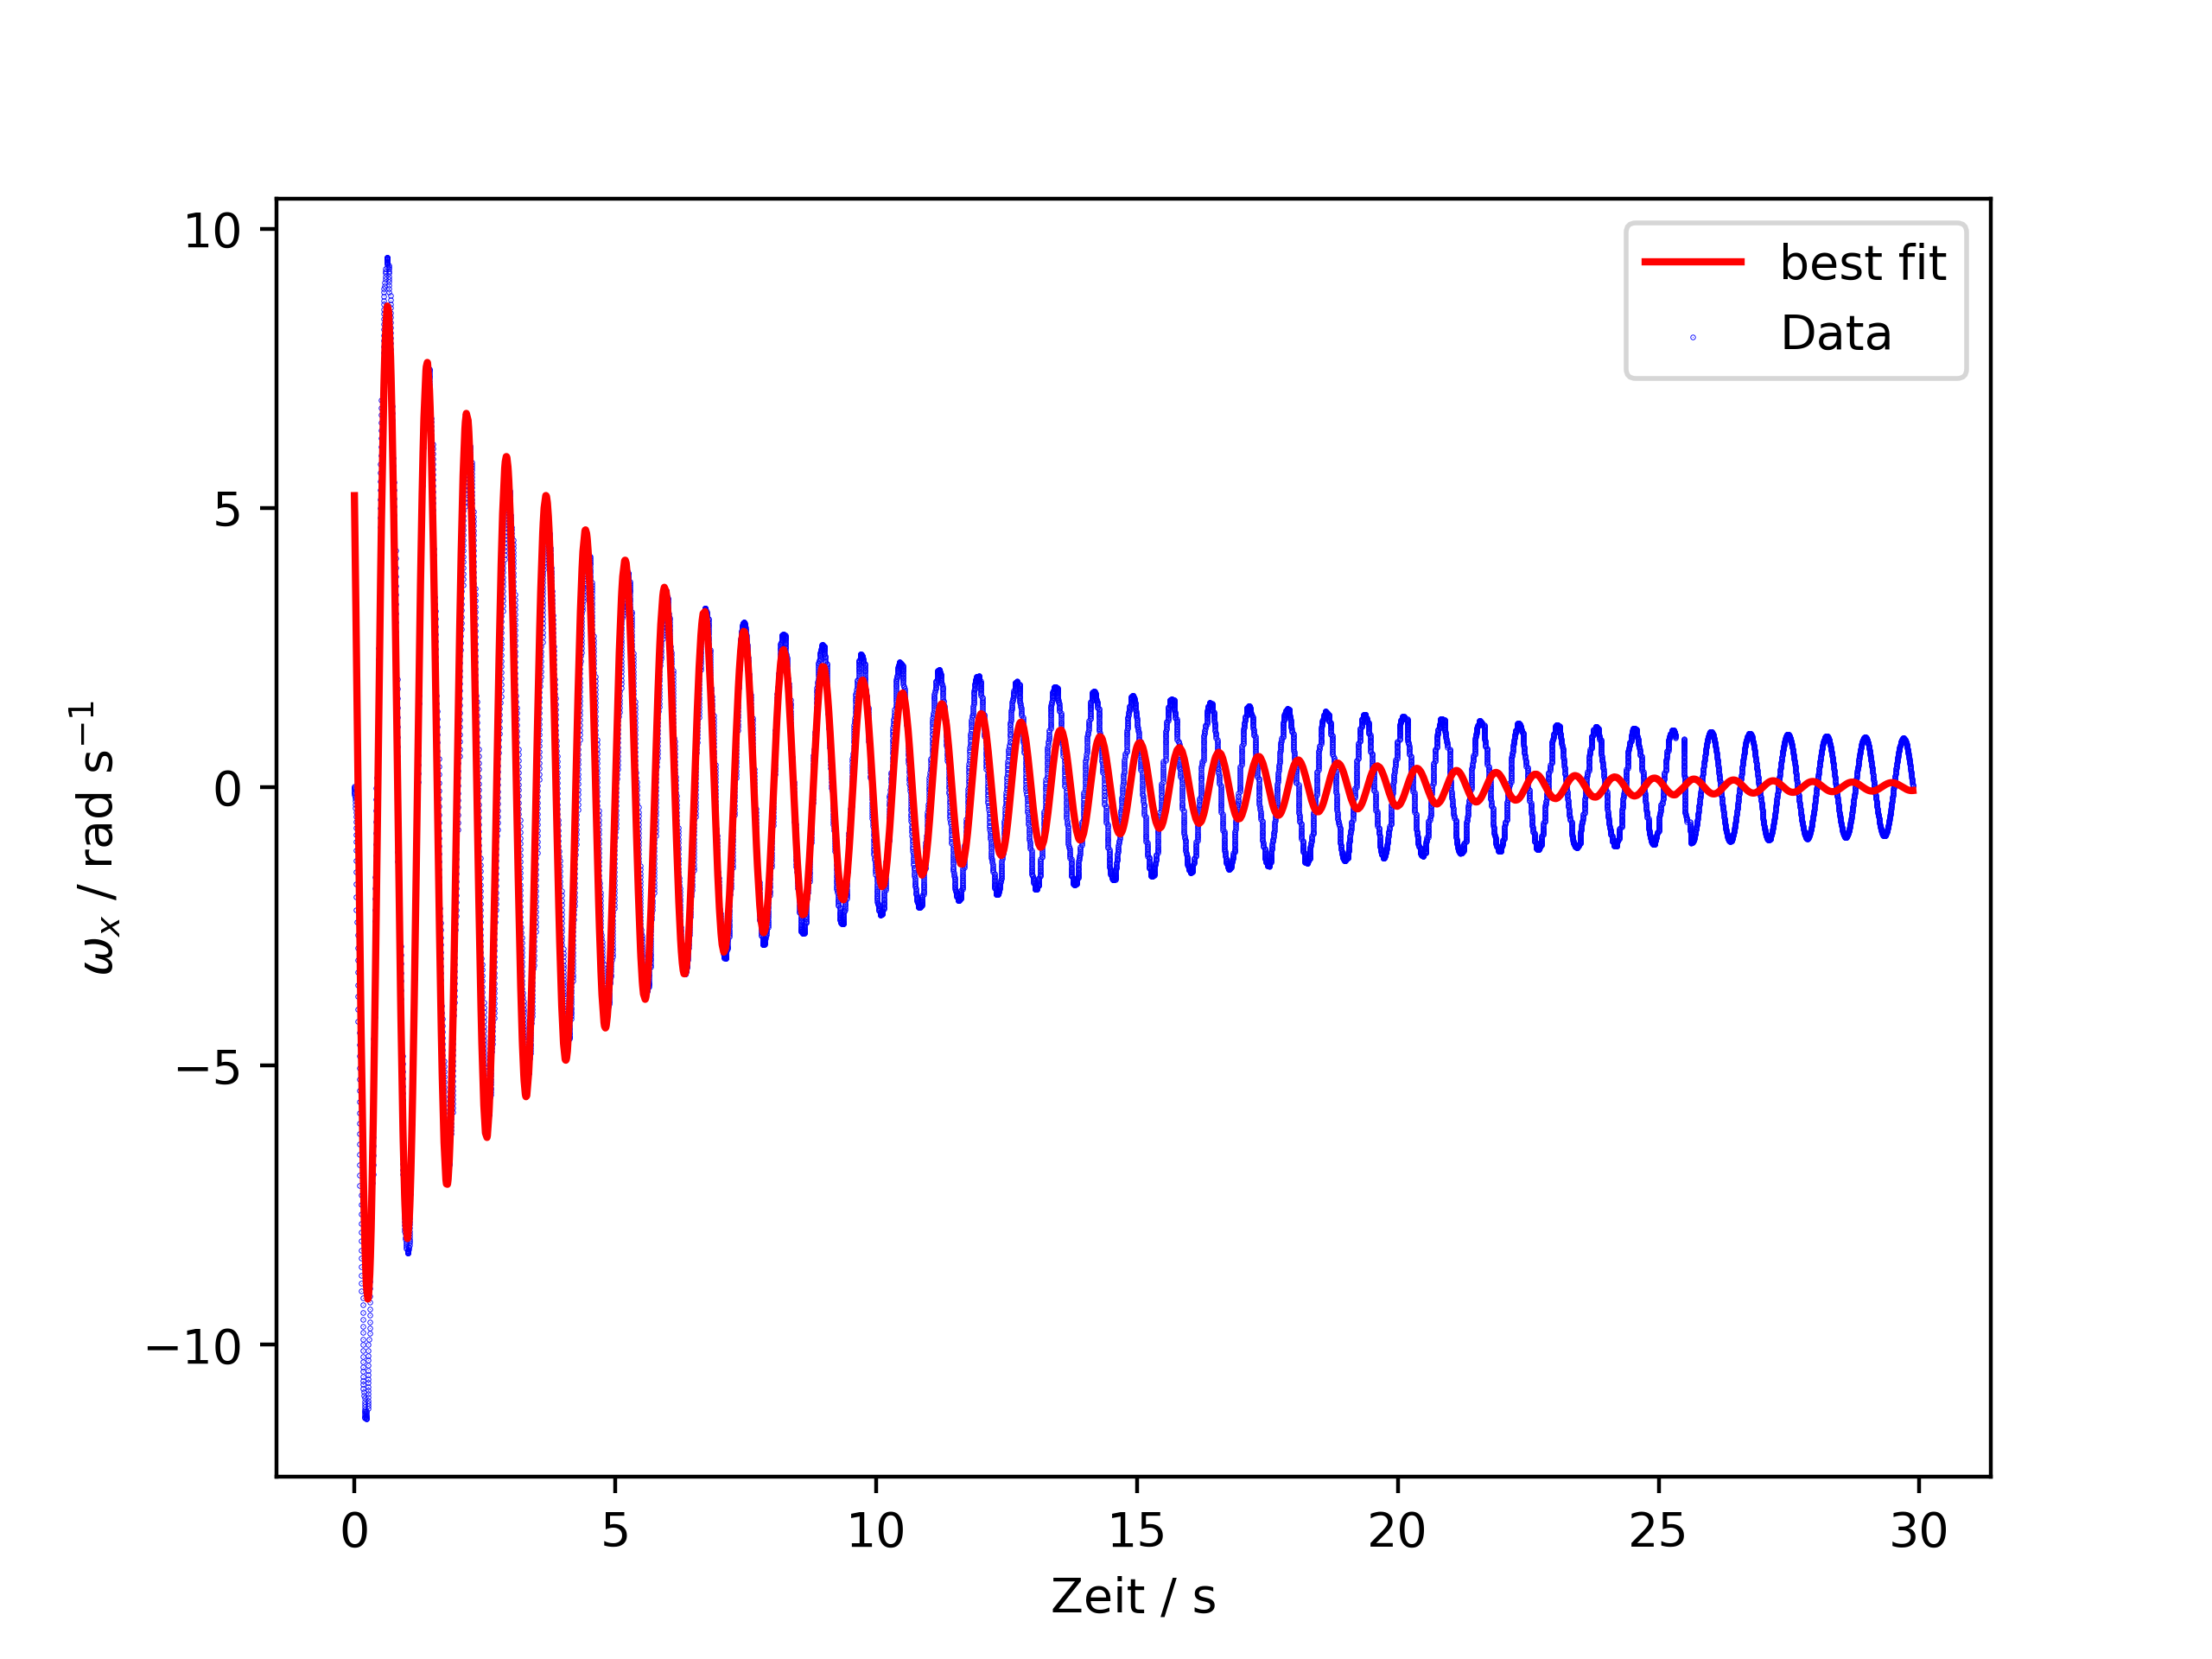
\includegraphics[width=0.8\linewidth]{pics/nonexp.png}
    \caption{Die gefittete Kurve (in Rot) für die Winkelgeschwindigkeit $\omega_x(t)$ 
    in Abhängigkeit von der Zeit, beschreibt nur den Anfang gut danach gibt
    es keinen expontienellen Abfall mehr}%
    \label{fig:nonexp}
\end{figure}

Ein Grund für diesen Übergang ist, dass am Anfang der Luftwiderstand
diesen expontienellen Abfall erst verursacht und ab einer gewissen
Winkelschwingung nichts der Abbremsung mehr beiträgt. Wenn die,
von der Winkelgeschwindigkeit, Abhängigkeit der Reibung bei
kleinen Winkelgeschwindigkeiten verschwindet, kann nur noch eine
konstante (lineare) Reibung die Winkelgeschwindigkeit verringern,
was in \autoref{fig:ubergang_exp_lin} zuerkennen ist.

\begin{figure}[H]
    \centering
    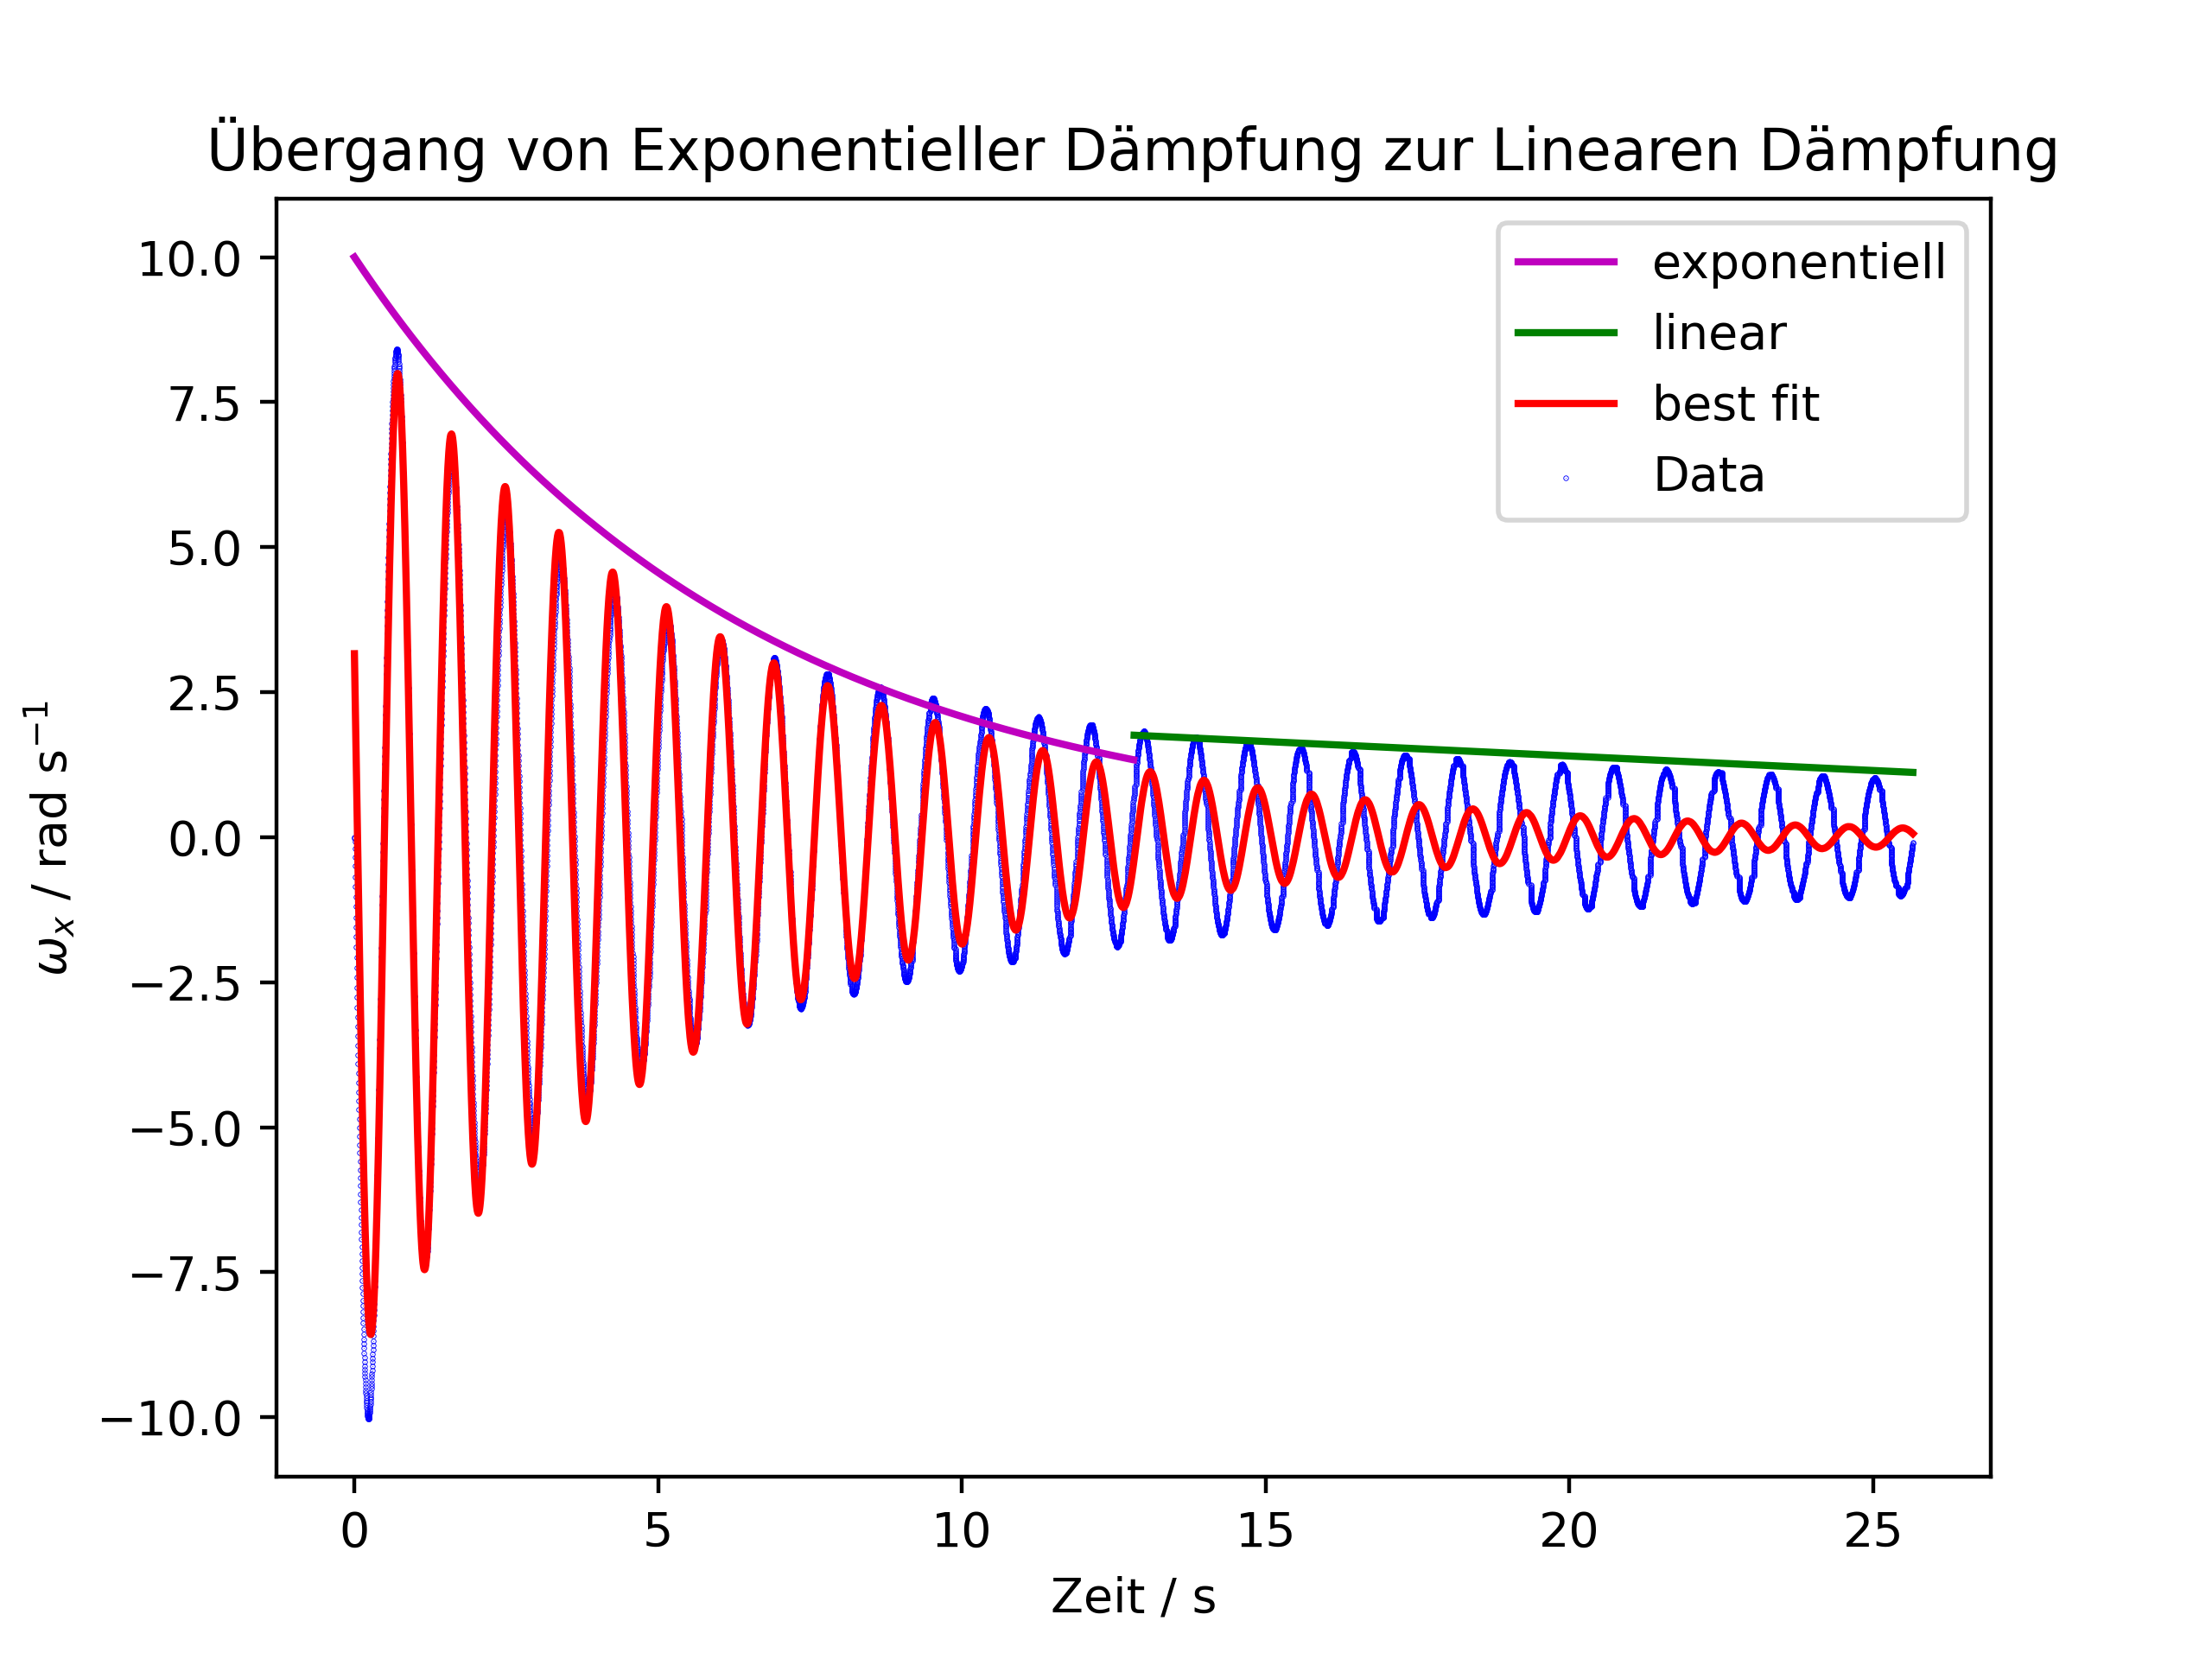
\includegraphics[width=0.8\linewidth]{pics/ubergang_exp_lin.png}
    \caption{Die gefittete Kurve (in Rot) für die Winkelgeschwindigkeit $\omega_x(t)$ 
    in Abhängigkeit von der Zeit, beschreibt nur den Anfang gut danach macht es
    einen Übergang von expontienellen Abfall (in Magenta) zu einem linearen Abfall
    (in Grün)}%
    \label{fig:ubergang_exp_lin}
\end{figure}

Eine weiter Erklärung für diese Diskrepanz könnte sein, dass durch das weite
Auslenken von \SI{90(2)}{\degree} Randeffekte stattfinden.

Nun zu dem Direktionsmoment $D_r$ dies konnte durch das Fitten bestimmt werden
um den erhaltenen Wert zu Vergleichen wurde der Wert auch mit
\autoref{eq:direktion} bestimmt.  Dazu ist der Radius $r=\SI{0.40(3)}{\mm}$ von
Hersteller \cite{stahldraht} entnommen worden, der Schubmodul für Stahl
$G=$ \SIrange{79.3}{81.0}{\GPa} von Wikipedia \cite{wikiSchubStahl} und
die Länge $l=\SI{35.0(5)}{\cm}$ wurde mit einem Maßband bestimmt.
Folgender möglicher Wertebereich wurde für das Direktionsmoment
gefunden:

\begin{equation}
    D_r = \text{\SIrange{6}{13}{\mN\m}}
\end{equation}

Der gefittete Wert für das Direktionsmoment $D_r$ liegt genau in
der Mitte des mit der \autoref{eq:direktion} errechnten Wertebereichs.

Weitere Vergleiche können nicht Vollzogen werden, da keine
Literaturwerte für die anderen Werte zufinden waren.

Damit bessere Werte gefunden werden können sollte,
man vielleicht das Smartphone weniger weit Auslenken.
Weiters könnte man die Münzen besser befestigen und
somit die Distanz von Schwerpunkt der Münze zur
Drehachse besser bestimmen.

\subsection{Zusammenhang}

Da $D_r$ größenordungsmäßig in dem Wertebereich liegt
lässt sich auch sagen, dass der Wert für das Trägheitsmoment
des Smartphones auch größenordungsmäßig dem realen Wert entspricht.

% Literaturtabelle
\newpage
\printbibliography

\listoffigures

\listoftables


\end{document}
